\section{Chapter introduction}

Considering its impacts on the energy budget at the surface, the effects of irrigation follow a marked diurnal cycle, with distinct effects in nighttime and daytime and varying amplitude depending on insolation. 
%option:could reuse ref from Intro
Average monthly or seasonal studies (like the work presented in Chapter \ref{chap:monthly}) cannot allow a detailed analysis of these impacts, and simulation outputs at a finer temporal resolution must be used.

Although it's based on the same simulation setup as Chapter \ref{chap:monthly}, this chapter focuses on the month on July 2021, and on part of the Ebro Valley. This study area and period were selected to include the measurement sites and special observation period (SOP) of the LIAISE field campaign. This enables direct comparison to local observations of temperature, humidity, wind and turbulent fluxes on irrigated and rainfed sites, at the surface and in the boundary layer. Furthermore, several mesoscale modelling experiments were conducted over this area and period, in particular using the mesoscale MesoNH model at 2-km resolution. These simulations served as an intermediate between punctual observations and the regional climate model, bringing new perspective on the following questions:

\begin{itemize}
    \item How does the ICOLMDZOR-LAM perform over the LIAISE study area, relative to observations and mesoscale simulations?
    \item To what extent does simulated irrigation improve the performance of the LAM? What limits its ability to reproduce observations on irrigated and rainfed sites at the diurnal scale?
    \item Are the effects of simulated irrigation limited to surface variables or do they propagate to the vertical structure of the ABL? 
    \item Are the effects of simulated irrigation only visible over the irrigated areas or do they also affect neighbouring rainfed areas?
    \item Over such a heterogeneous terrain, how can representativity of the LAM be defined and to what extent is it achieved?
\end{itemize}

This chapter first presents the LIAISE field campaign with details on the measurements used, mesoscale simulations that were conducted over the study area, and the main results of this project.
Then, the ICOLMDZOR LAM simulations used for comparison over LIAISE sites are described, before presenting results on land-atmosphere coupling variables and the vertical structure of the atmosphere.
%todo: improve/rephrase after final structure

\section{The LIAISE field campaign}
This description of the Land Surface Interactions with the Atmosphere over the Iberian Semi-Arid Environment (LIAISE) project is partly based on the various articles which presented the campaign : \citet{boone_land_2019,boone_updates_2021,boone_land_2025}, as well as on the dedicated section in Tanguy Lunel's PhD thesis \citep{lunel_interactions_2024}.

%objectives
LIAISE is an international research campaign aimed at improving the understanding of land-atmosphere-hydrology interactions in a semiarid region characterized by strong surface heterogeneity owing to contrasts between the natural landscape and irrigation-dependent agriculture, and the limitations of models to represent all aspects of the terrestrial water cycle.

%period
Although the campaign included a longer monitoring of surface variables, this work focuses on the special observation period (SOP) which occurred from July  15–29 2021. This SOP has been selected since it is the period where contrasts between irrigated and natural surfaces are generally at or near their maximum. At this time, synoptic scale winds are typically light and from the west, and a  thermal (heat) low pressure area generally forms over the region with daily maximum temperatures in the mid-to-upper  30s °C.
Within this SOP, Intensive Observation Periods (IOPs) were selected, aiming for relatively clear days characterized by a well-mixed  atmospheric boundary layer with weak synoptic scale forcing, so that surface-induced local to regional scale circulations were most likely to be present and detectable. 

%area
The study domain for LIAISE is the Ebro basin in northeastern Spain, which is bound to the north by the Pyrenees and to the south by the Iberian System.
It presents a semiarid hot, dry  Mediterranean climate, with a very sharp delineation between a vast, nearly continuous intensively-irrigated region and the generally drier rainfed zone to the east of the study domain.
%sites
Two supersites were defined at La Cendrosa, within the irrigated zone, and Els Plans, within the rainfed zone. Each was equipped with a 50-meter mast to measure temperature, humidity, wind speed, radiative and turbulent fluxes (using eddy-covariance) at various heights.
This work used 2-meter measurements for most variables, and 10-m wind speed.
On IOP days, hourly radiosondes were launched, roughly from  sunrise through early evening, probing the ABL up to about 3 km.

\begin{figure}[hbtp]
    \centering
    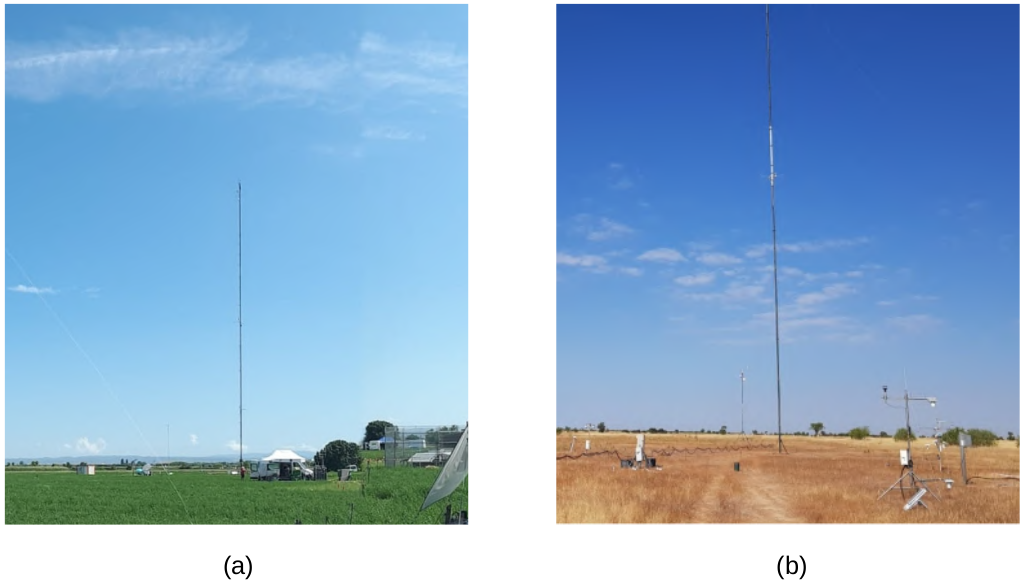
\includegraphics[width=\textwidth]{images/chap5/liaise_sites_picture.png}
    \caption{Instrumented sites of La Cendrosa (a) and Els Plans (b) in July 2021 \citep[taken from ][]{lunel_interactions_2024}.}
\end{figure}



%choice of IOP days, synoptic conditions
%  This thermal situation has  a strong impact on surface winds. Formation of some shallow cumulus is possible, but moist convection, if present, is  generally confined to the surrounding mountain ranges. Owing to the proximity to the Mediterranean Sea to the east, sea  breeze (SB) formation is quite frequent, but its inland progression is slowed by the presence of the Catalan pre-coastal and  coastal ranges that separate the Ebro basin from the sea. The  intensity of the westerlies and strength of the heat low are also  contributing factors to the SB front propagation and intensity. Generally speaking, the SB front usually arrived sometime  between 16:00 and 19:00 local time over the study zone with  the dry zone sites impacted earliest. The SB passage was seen  in the observations as a low level wind shift (to winds with a  significant easterly component) over the entire region, while in  the east, horizontally-scanning lidar observations also revealed  a significant increase in low-level moisture with its arrival. The  sea breeze generally coincided with a collapsing ABL in the late  afternoon. Days with a predicted early arrival of the SB were  not designated as IOPs during the daily briefings. Finally, one  rain event did occur on July 26, which was associated with the  passage of a synoptic scale trough: local precipitation totals of  around 30 mm were recorded over the irrigated zone; however,  the convective cells propagated to the northeast and the dry  zone received relatively little rainfall, thereby reinforcing the  wet-dry zone contrast during the subsequent days of the SOP.

%measurements / instruments
%irrigation practices and timing. Urgell canal adduction
%overview of synoptic conditions, rainfall
% simulation experiment with conceptual and mesoscale models
%main outcomes so far : Mangan, Lunel (2 sites), Lunel Marinada, intermodel comparison

%option:voir si irait bien quelque part: 
%Most of the water used for agriculture, approximately 75%, is stored in reservoirs while the rest is maintained by the snow pack in the mountains.


\section{Simulation experiments}

Several simulations are compared to analyse the diurnal cycle of land-atmosphere coupling variables in the Ebro Valley.
First, the two simulations studied in Section \ref{sec:article1} (\noirr and \irr) were analysed and compared to LIAISE observations using hourly outputs over the month of July 2021.

Then, sensitivity experiments were conducted to increase irrigation over grid cell corresponding to the irrigated site of La Cendrosa, leading to the simulation henceforth referred to as \irrboost. This simulation was only run over the month of July, starting from the same state as \noirr and \irr on July 1st 2021, and involved significant changes in both on the computation of irrigation demand, and on the water availability. 
Regarding demand, the irrigated fraction was slightly increased to make sure that all of the soiltile dedicated to low vegetation and crops was considered as irrigated land. This soiltile represents 83.5\% of the grid cell, the rest being occupied by trees (12.4\%) and bare soil (4.1\%). This fraction was also reduced to 0\% on the Els Plans site to make sure there would be no irrigation demand computed in this grid cell.
More importantly, the \betairrig parameter, which had been set to 0.6 after the offline calibration in Chapter \ref{chap:routing} to avoid excessive depletion of the groundwater and river reservoirs, was increased to 1. This means that the irrigation scheme is aiming to maintain soil moisture in the root zone (first 64cm of soil) to field capacity, making sure that plants would not be limited in their growth by available soil moisture. 
Regarding available water, since this was a short simulation run (one month), very large amounts of water were added in the three routing reservoirs at the simulation initial state, making virtually inifinite amounts of water available for irrigation in the LIAISE region. Obviously, this method is not realistic, nor applicable to longer climate runs, and was only used to test the limits of the irrigation scheme and explore the sensitivities of land-atmosphere interactions in a context where irrigation would be driven by the water demand rather than the supply. 
When comparing to reality, this can also be seen as a way to compensate for the absence of water adduction in the ICOLMDZOR LAM simulations, a practice that is determinant in the actual supply of irrigated water in the area. %todo:see if this explained in previous sec, refer to it
%todo:see also if irrigation simulation method used by tanguy has been detailed (because that's what it does too)

The three ICOLMDZOR LAM simulations (\noirr, \irr, \irrboost) are compared to observations and to the MesoNH simulation from July 14th to July 30th. This covers all the LIAISE SOP and allows for the stabilization of irrigation volumes in the \irrboost simulation, since no long-term spinup was conducted with this setup.

\hfill

%todo:choice of grid cell -> figure
For each site, an ICOLMDZOR grid cell was selected for the comparison to observations. For Els Plans, the grid cell containing the exact site location seemd appropriate since it was a very lightly irrigated cell. however, the exact position of the La Cendrosa site was not in an intensely irrigated cell, which is why the neighbouring grid cell was selected.

%fig:sites and corresponding grid cells
\begin{figure}[hbtp]
    \centering
    \begin{tabular}{cc}
        \begin{subfigure}[t]{0.44\textwidth}
            \caption{Visible image of the LIAISE study area as seen by \textit{Sentinel-2} on July 22nd.}
            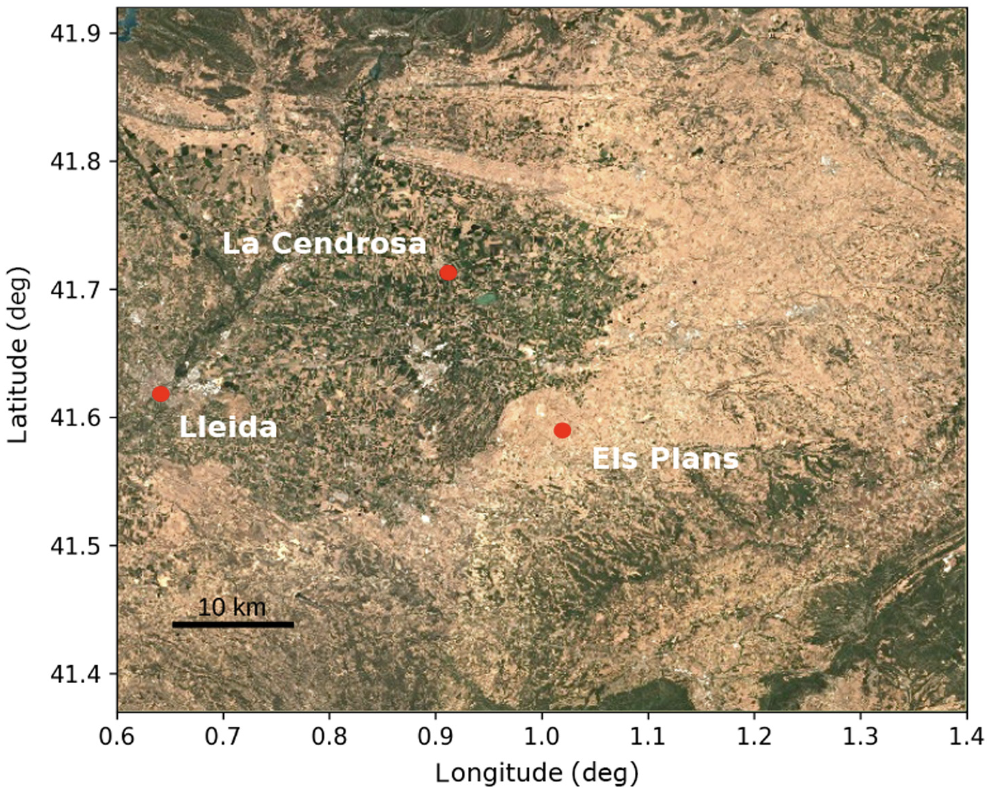
\includegraphics[width=\textwidth]{images/chap5/liaise_overview_lunel.png}
        \end{subfigure} &

        \begin{subfigure}[t]{0.5\textwidth}
            \caption{Monthly average irrigation simulated by ORCHIDEE (July 2021, \irr simulation).}
            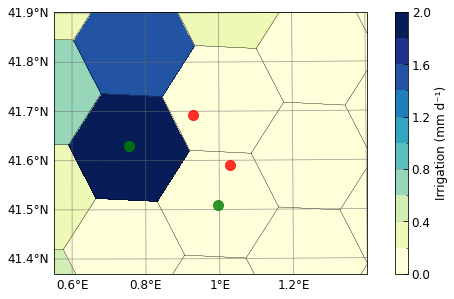
\includegraphics[width=\textwidth]{images/chap5/liaise_sites_irrig_ORC.png}
        \end{subfigure} 
    \end{tabular} 

    \begin{subfigure}[t]{0.75\textwidth}
            \caption{Average latent heat flux simulated by MesoNH (14-30 July 2021, with irrigation). Red hexagons show the ICOLMDZOR grid cells for each site.}
            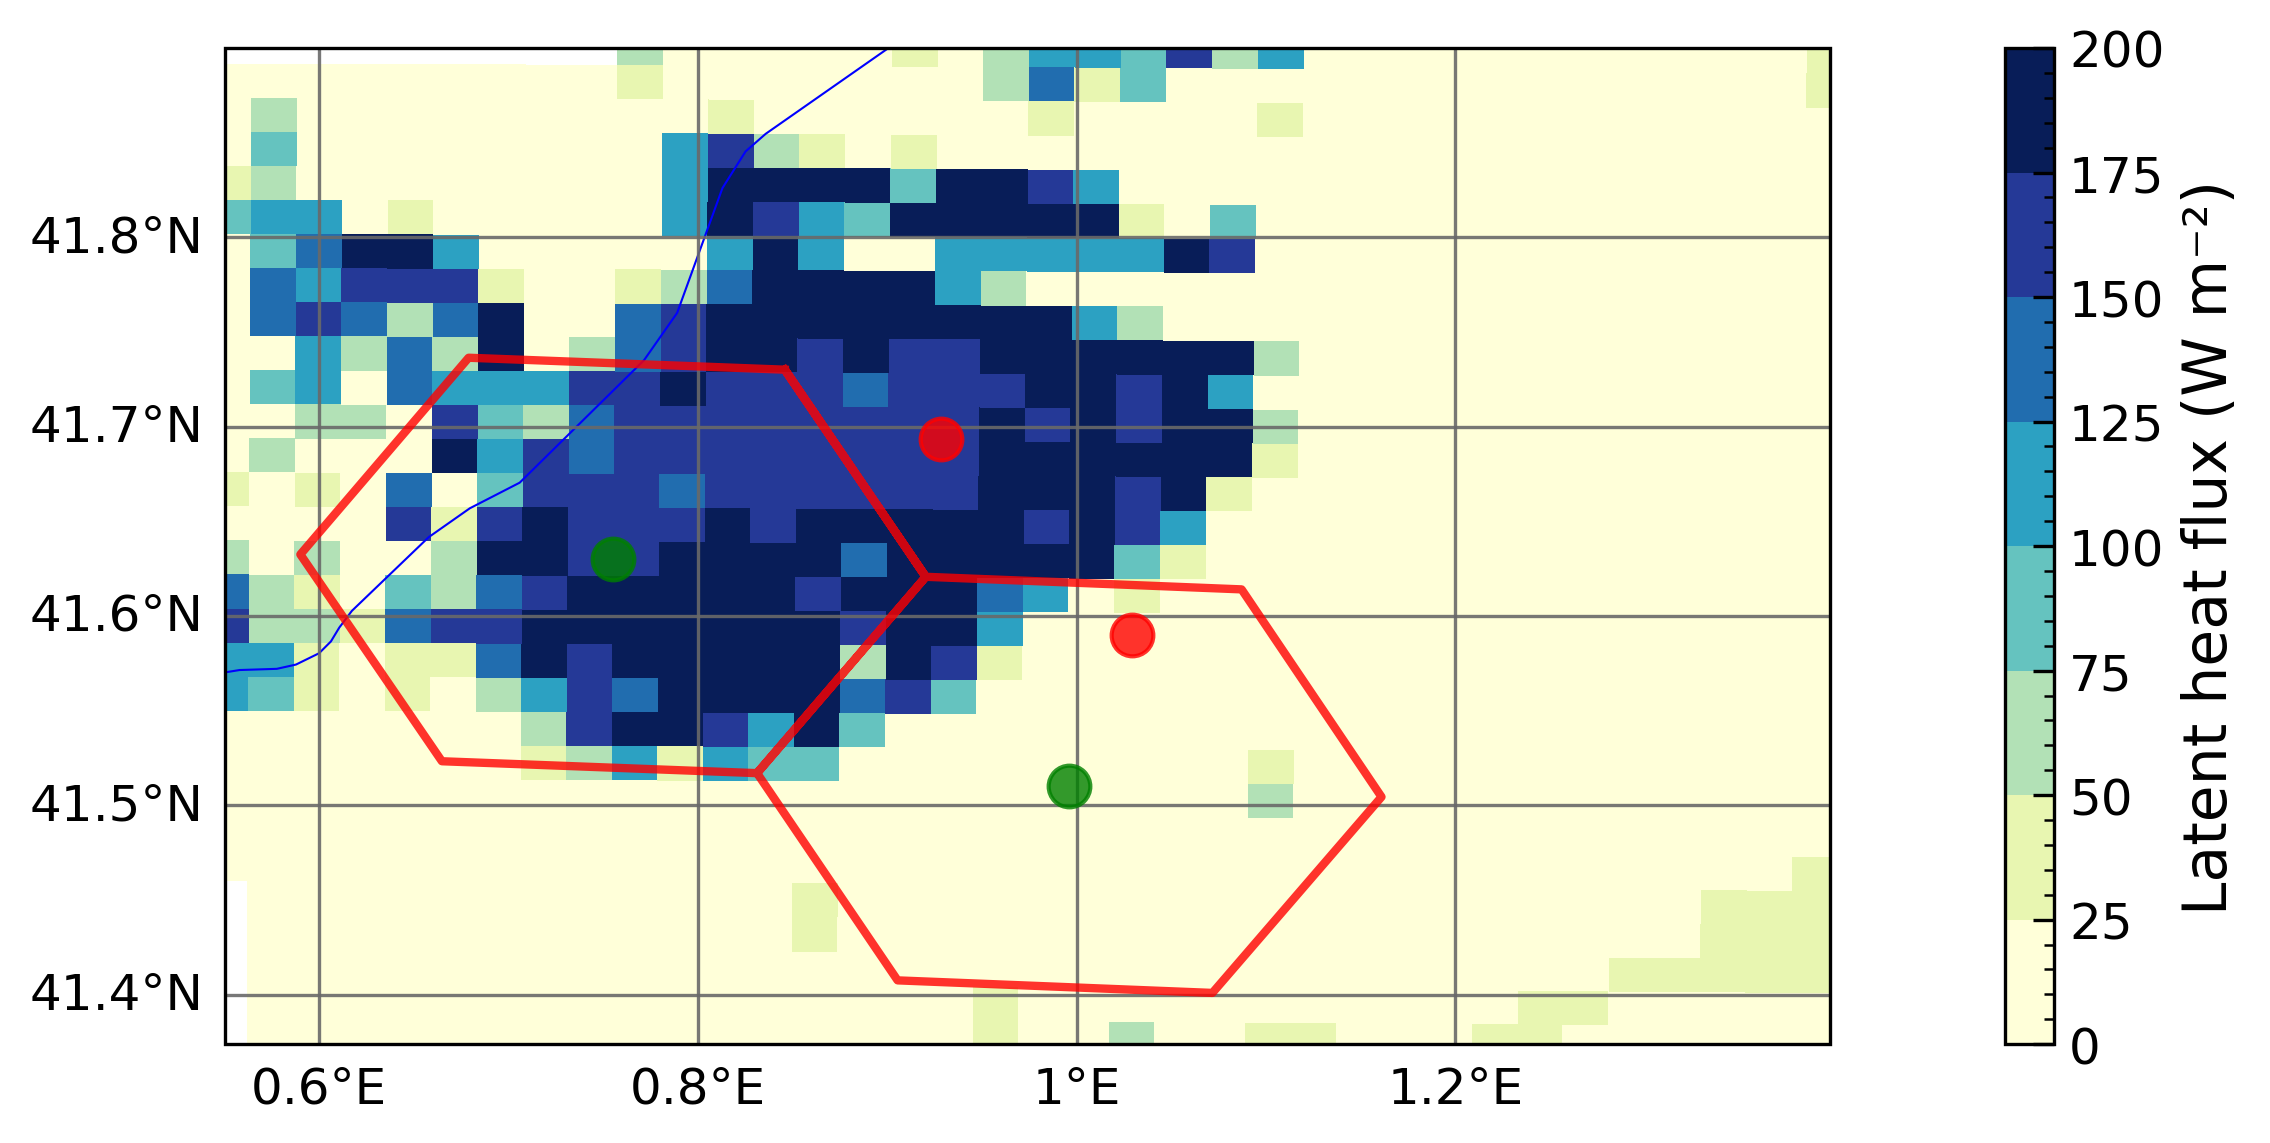
\includegraphics[width=\textwidth]{images/chap5/liaise_sites_mean_mesoNH.png}
        \end{subfigure} 
    
    \caption{Correspondance between actual location of La Cendrosa and Els Plans sites (red dots), selected ICOLMDZOR grid cells (centered on green dots), and MesoNH grid. (a) was taken from \citet{lunel_irrigation_2024}.}
    \label{fig:liaise_sites_grid_cells}
\end{figure}

%todo:mesoNH (if not presented in previous section ?)
Comparison to the MesoNH simulations was performed using two values for each site. 
The first one, referred to as \mesoexact, takes the variables from the exact grid cell corresponding to the site location based on the GPS coordinates of the site, as done in \citet{lunel_irrigation_2024}. 
The second, referred to as \mesomean, is an aggregation of all the MesoNH grid cells contained into the selected ICOLMDZOR grid cell for each site. The mean value is shown, as well as an envelope encompassing the 25th and 75th percentiles, when it is appropriate.
On Fig. \ref{fig:liaise_sites_grid_cells}c, the two hexagonal ICOLMDZOR grid cells are drawn upon the average latent heat flux simulated by MesoNH. It can already be noticed that within the grid cell for La Cendrosa, there are some MesoNH grid cells with very low values of ET, and that in the grid cell for Els Plans, there are some MesoNH grid cells which fall into the irrigated zone and exhibit high ET. This will have an influence on the \mesomean values and on the spread of MesoNH surface variables within one ICOLMDZOR grid cell. 
%option:mesoMean is not meant to be more representative of the obs than mesoExact, but to bring information on heterogeneity within one ICOLMDZOR grid cell

\section{Surface variables over the SOP}
\label{sec:sop}

Here, surface variables simulated by ICOLMDZOR and MesoNH are compared to the observations on both sites from July 14th to July 30th (the span of the MesoNH simulation), which corresponds to the LIAISE SOP.

At La Cendrosa (Fig. \ref{fig:cendrosa_surfacevars}), turbulent fluxes exhibit clear diurnal cycles piloted by solar irradiation, with a maximum value between 12 and 13UTC.

%%LA CENDROSA%%
%turbulent fluxes
%noirr has almost no flat and largely overestimates fsens (300%)
%these biases are reduced in irr, which follows a good trajectory at the beginning of the day, but lacks water to sustain irrigation demand
%in irrboost, DC structure is normal, irrigation demand is sustained throughout the day and biases on turbulent fluxes are largely improved compared to obs
%mesoExact is not that good on flat DC because of overestimation in the beginning of the SOP -> link to vegetation development
%mesoExact if fine on sensible heat flux, also due to a partial error compensation over 15 days
%irrboost is very close to mesoMean for both turbulent fluxes, meaning the average grid cell flux simulated by ICOLMDOR performs very well, if mesoNH sim is considered a good reference.

%t2m
%DC of t2m is also driven by radiation and turb fluxes, the peak is shifted in the afternoon. 
%all model sim exhibit a warm bias, especially at night, where even mesoExact is closer to ICOLMDZOR than to observed values.
%warm bias in noirr is reduced in irrboost (2° at peak) which follows mesoMean for most of the day

%q2m
%DC less structured, variable more sensitive to wind (mixing and advection)
%LAM is not good in daytime, dries very fast (link to wind, overestimated in the day ?), bias reduced with irrig. Irr boost fall within spread of mesoMean but structure still far from good
%With irrig, LAM is better in nighttime whereas mesoNH underestimates. Possibly a feat of the irrigation parameterization which bring a little water at every tme step

%wind
%speed variations small but direction shift has a clear mean DC
%mesoNH very close to obs
%ICOLMDZ overestimates speed, partly improved with irr (LAI or ET ??)
%Variations of direction less pronouced in ICOLMDZ and mesoMean
%some afternoon variations (20-21-22) absolutely not captured by LMDZ whereas seen in obs and mesoExact (discussed later)

%%ELS PLANS%%
%Very different energy partitionning : latent heat flux lower than 20W/m² whereas sensible heat flux peak be 3x larger than in La Cendrosa
%ICOLMDZ underestimates latent heat flux and overestimates sensible heat flux
%very little difference between 3 LAM sims (a bit of irrig in irrboost due to the shape of the routing grid vs shape of ICOLMDZOR grid)
%mesoExact has a sharper latent heat flux peak than obs, and overestimates sens in the afternoon
%mesoMean strongly influenced by few outliers (mean above 75th percentile) for flat, reasonable for fsens, still far from ICOLMDZOR

%t2m q2m
%mesoNH overestimates nightime temp and underestimates daytime peak (even though more fsens ?)
%ICOLMDZOR good odg but early peak (as in La Cendrosa)
%q2m structure in obs different from La Cendrosa, minimal peak in afternoon
%q2m in ICOLMDZ look a bit like La Cendrosa... dominated by wind rather than local ET ?
%mesoNH underestimates q2m at night but shows less variations in the day so catches up with obs in daytime

%wind
%Stronger than La Cendrosa (roughness), clearer DC in obs and mesoNH
%DC structure in ICOLMDZ is good but speed underestimated
%direction shows less variations and is quite well reproduced by models on average, although some events are clearly missed (TS)

%%CCL%%
%irrigation param in ICOLMDZ can significantly improve the results for surface vars at La Cendrosa, especially when functioning without the limitation of available water
%Even if 4 vars don't reach the obs in irr_boost, they can be very close to the mesoMean, meaning they achieve the objective of representing the grid cell mean flux
%differences in q2m at La Cendrosa, daytime structure and dry bias
%possibly linked to excess wind that limits impact of local ET by mixing 
%At Els Plans, model quite good, overestimate sens but not t2m, dry bias in q2m (not linked to excess wind here)
%wind similar at both sites in ICOLMDZOR but differences in obs -> roughness ? larger sclae effects not seen in irr_boost because of irr structure ?

%discussion
% flat in irrboost is mostly driven by bare soil evap : realistic ? error compensation? need further developments in plant behaviour ?
%setup not good for dynamical effects, very strong irrig for some grid cells and no irrig at Els Plans


%fig : Cendrosa turbulent fluxes + t2m, q2m
\begin{figure}[hbtp]
    \centering
    \begin{tabular}{cc}
        \begin{subfigure}[t]{0.5\textwidth}
            \caption{}
            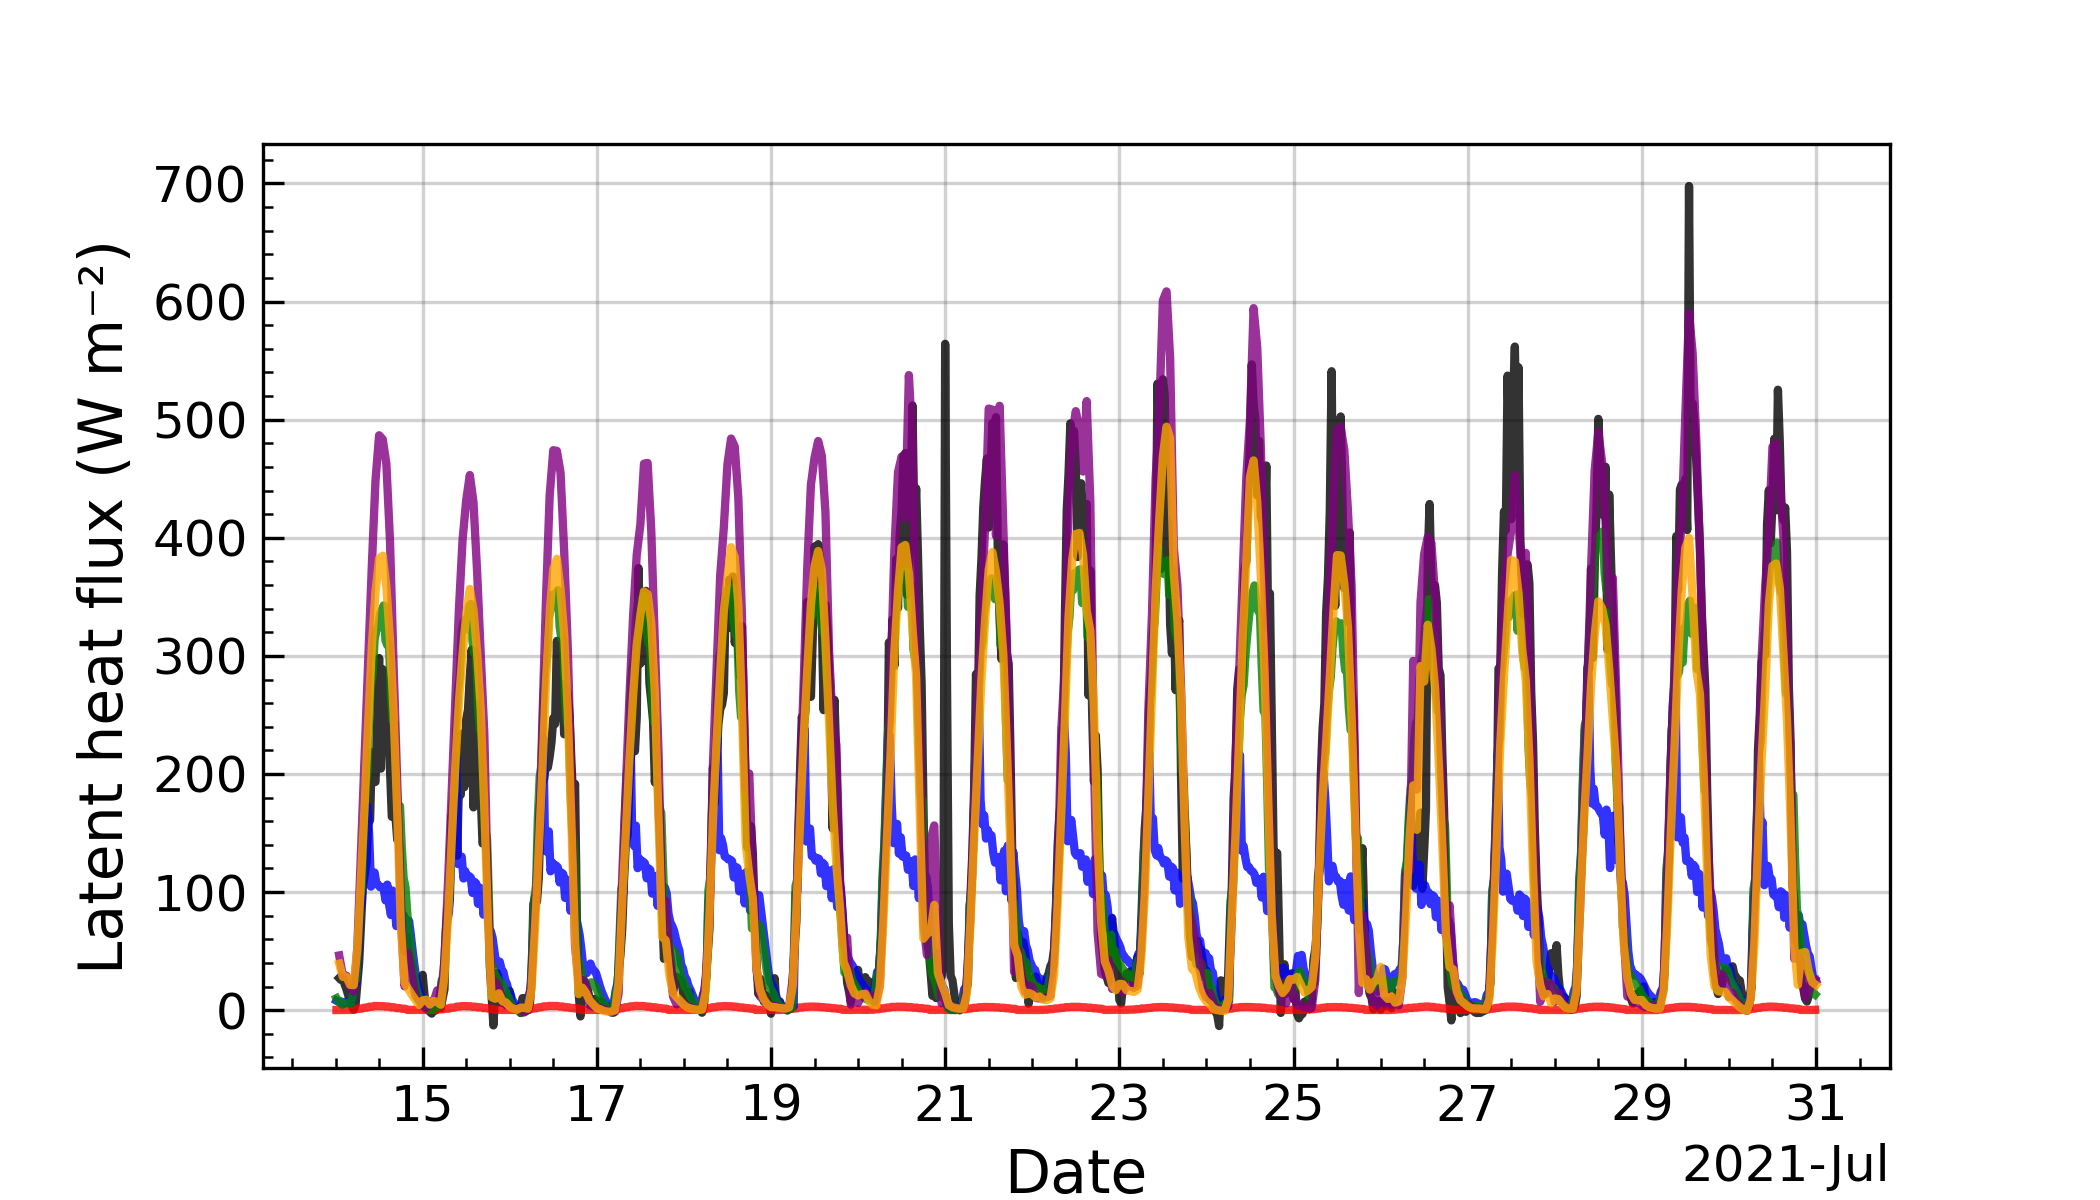
\includegraphics[width=\textwidth]{images/chap5/SOP_TS_DC/time_series_cendrosa_flat.png}
        \end{subfigure} &
        \begin{subfigure}[t]{0.5\textwidth}
            \caption{}
            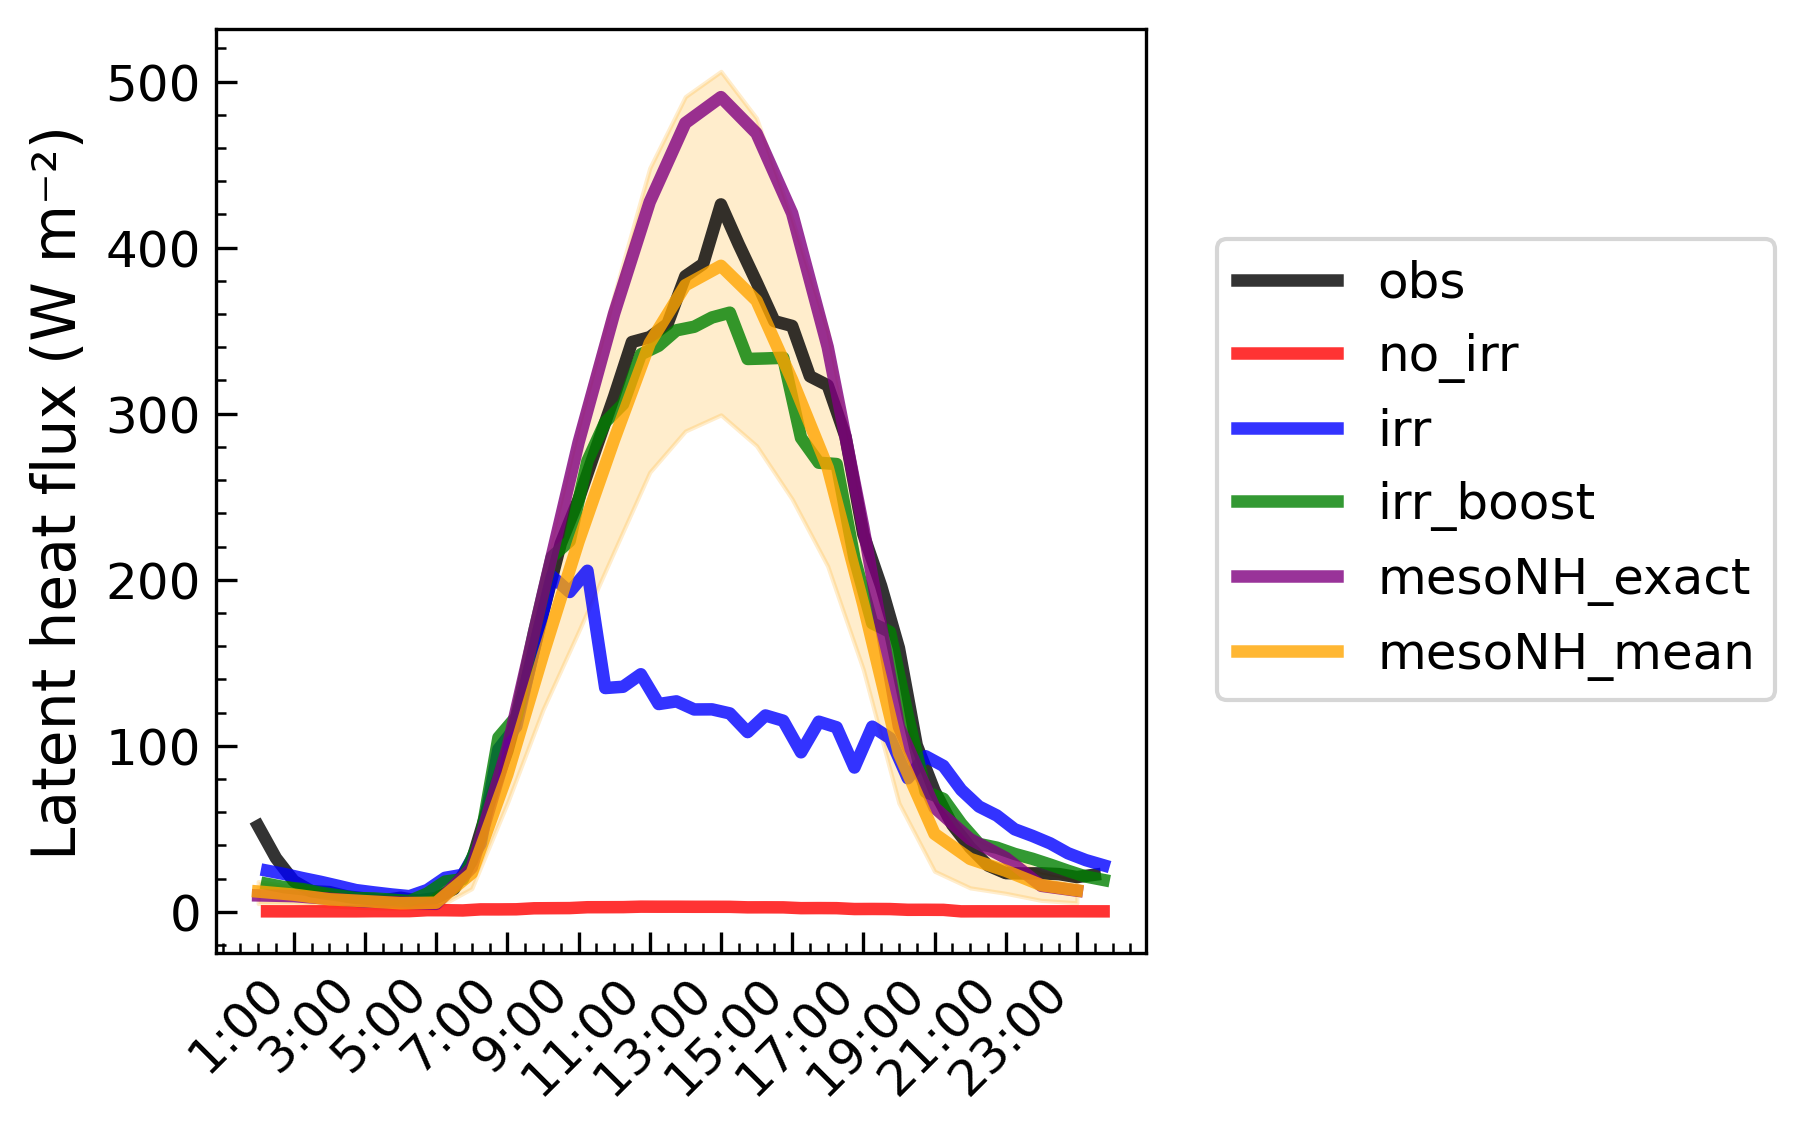
\includegraphics[width=\textwidth]{images/chap5/SOP_TS_DC/diurnal_cycle_cendrosa_flat.png}
        \end{subfigure} \\
        
        % \vspace{1em} % Add vertical space between the rows
        \begin{subfigure}[t]{0.5\textwidth}
            \caption{}
            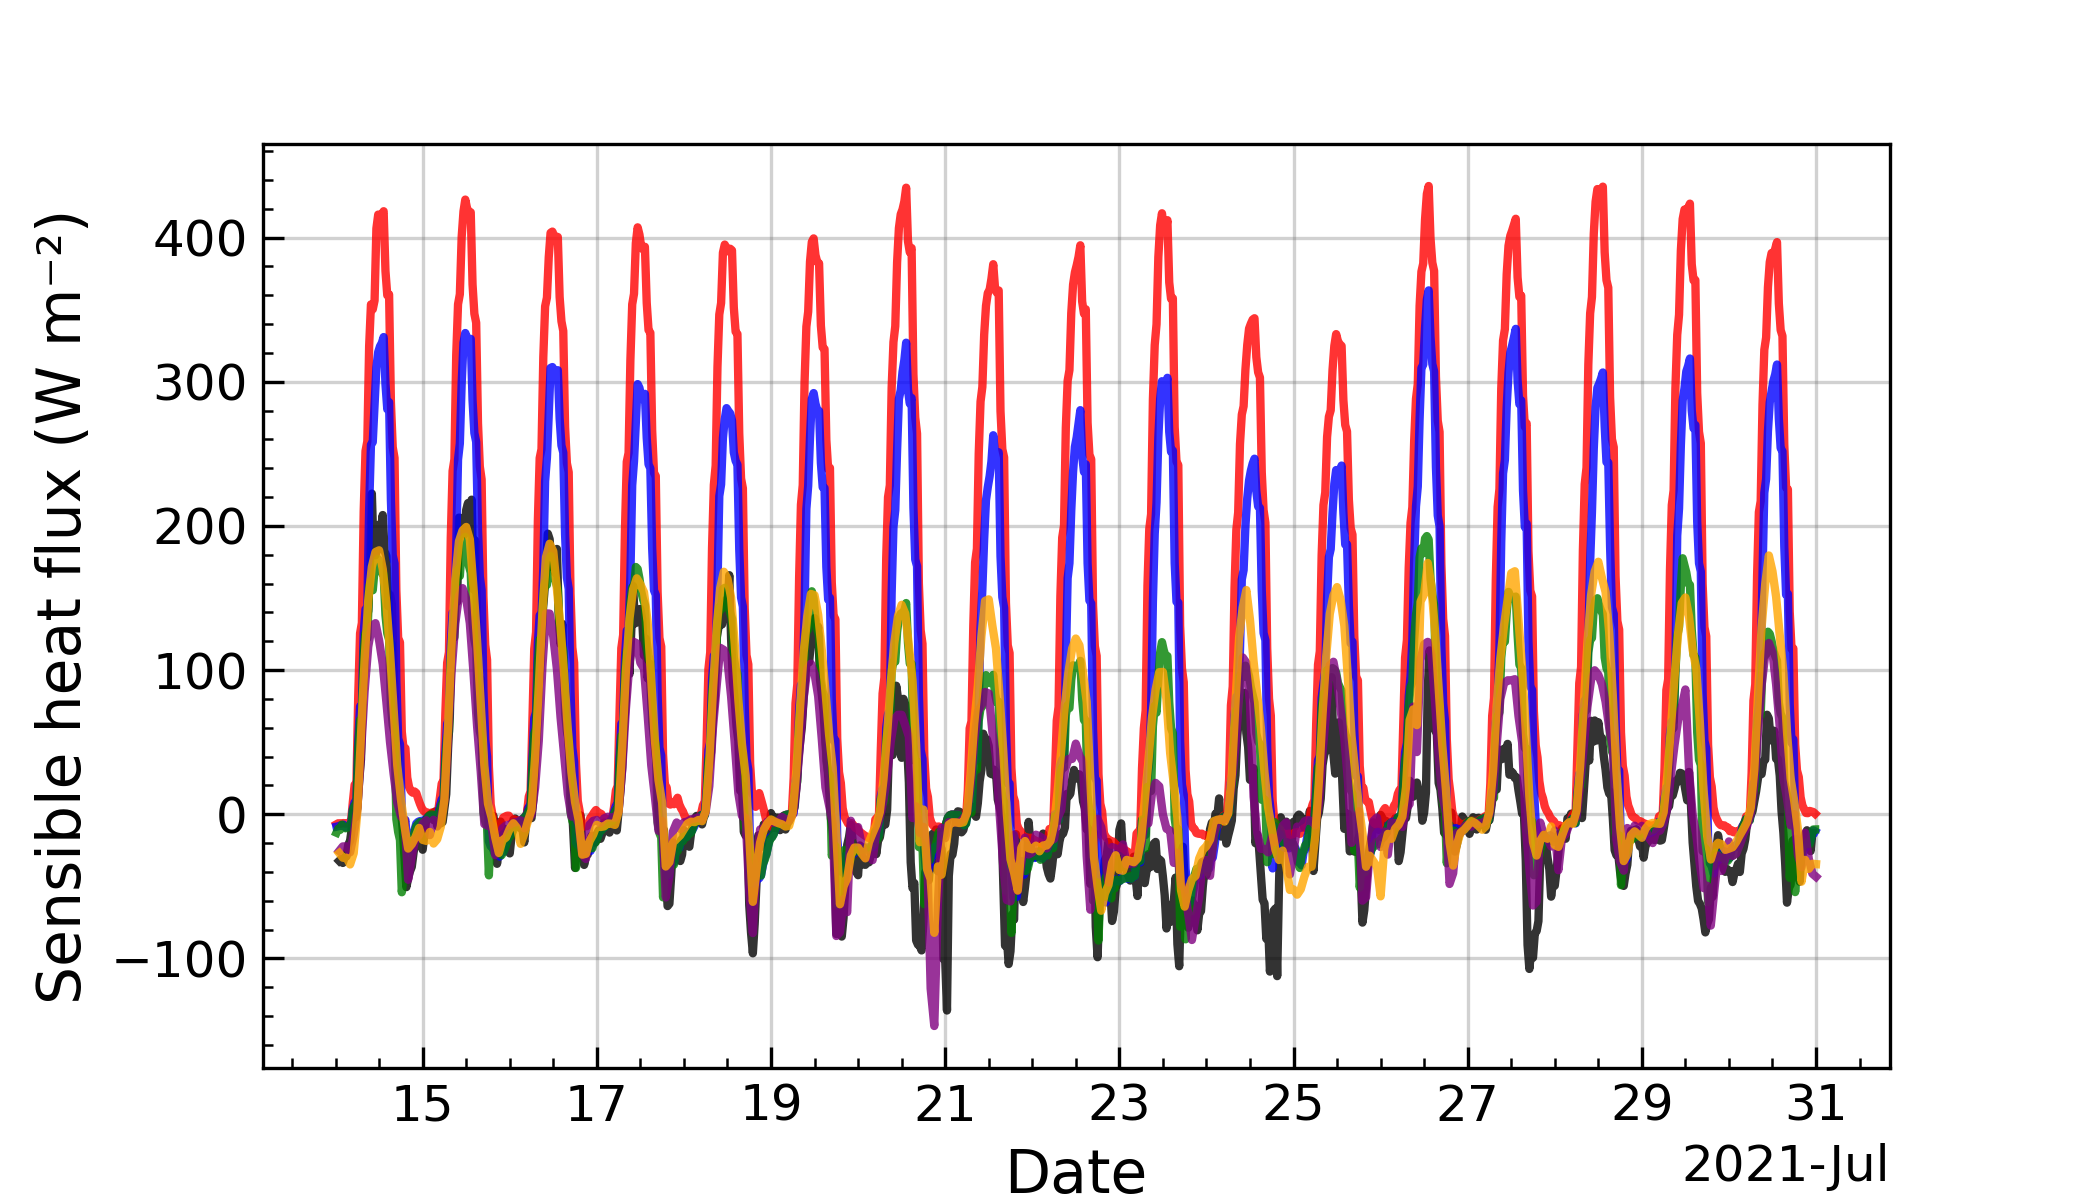
\includegraphics[width=\textwidth]{images/chap5/SOP_TS_DC/time_series_cendrosa_sens.png}
        \end{subfigure} &
        \begin{subfigure}[t]{0.5\textwidth}
            \caption{}
            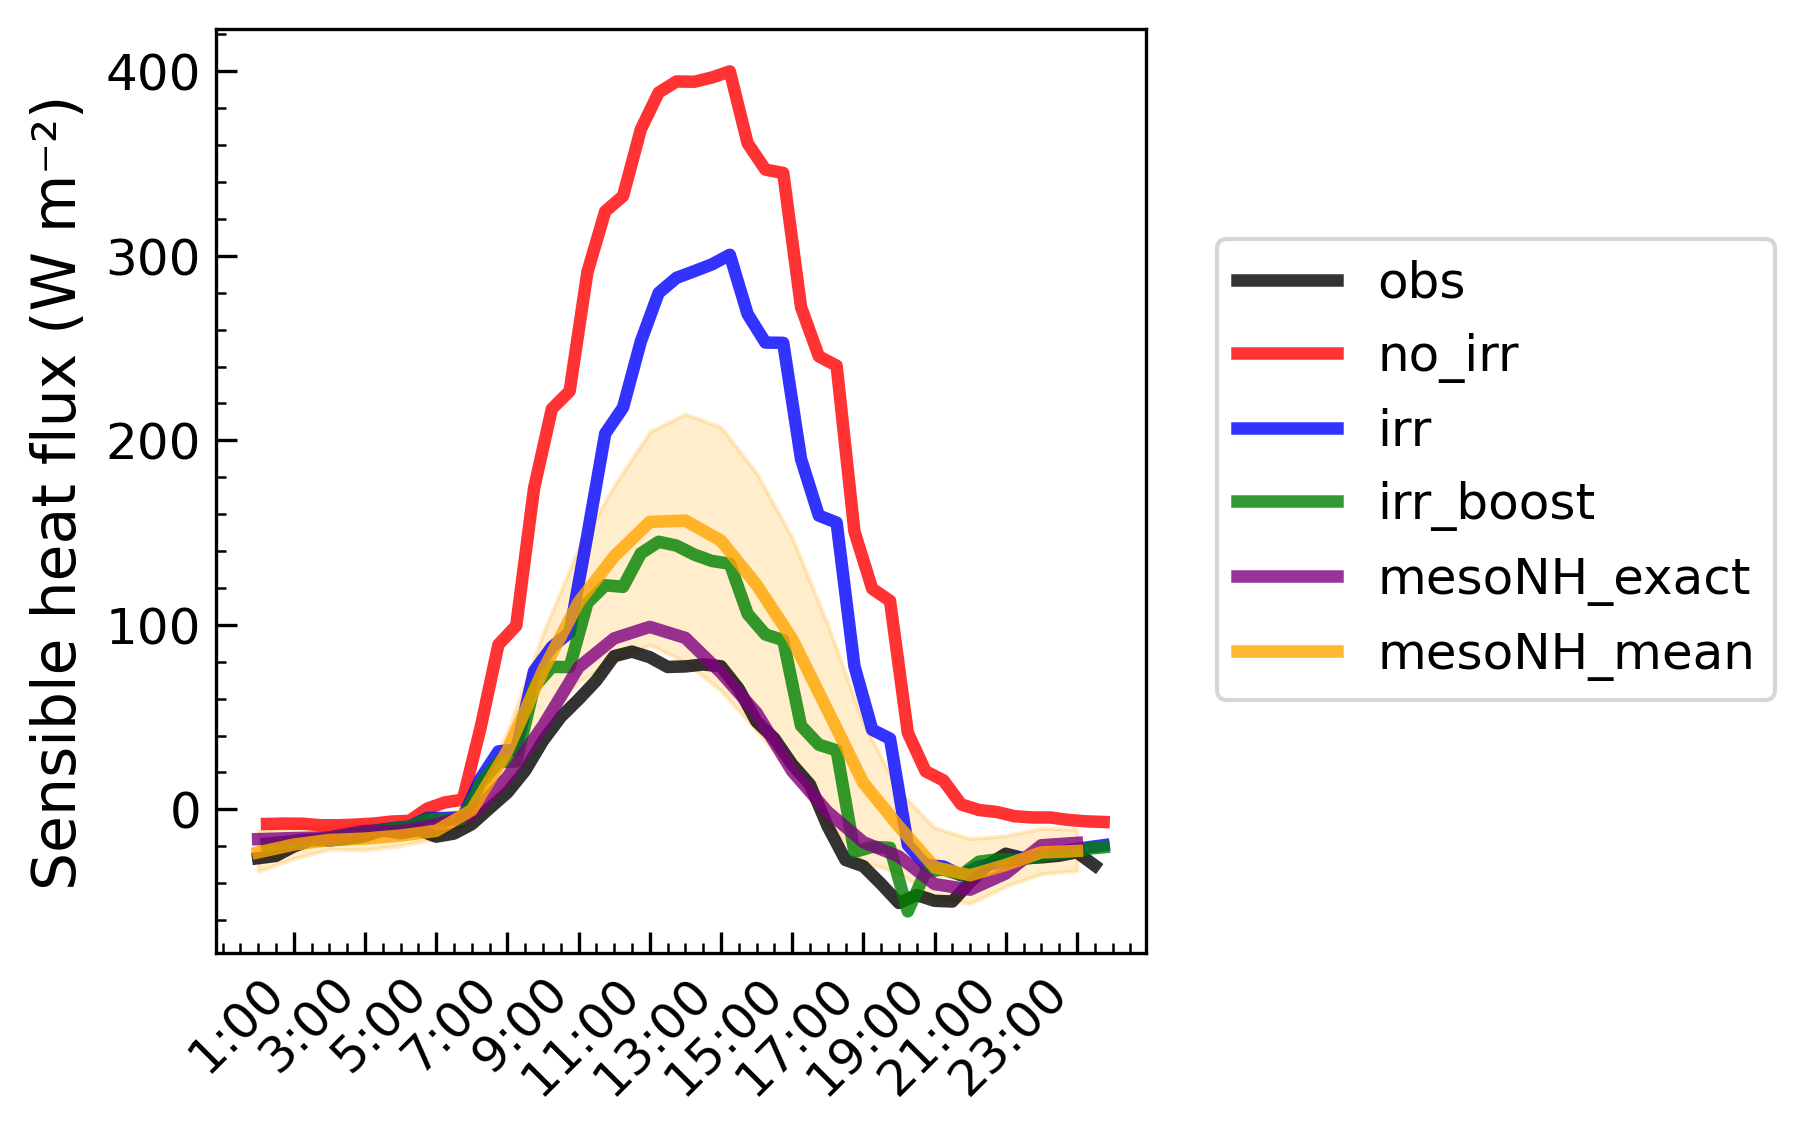
\includegraphics[width=\textwidth]{images/chap5/SOP_TS_DC/diurnal_cycle_cendrosa_sens.png}
        \end{subfigure} \\

        \begin{subfigure}[t]{0.5\textwidth}
            \caption{}
            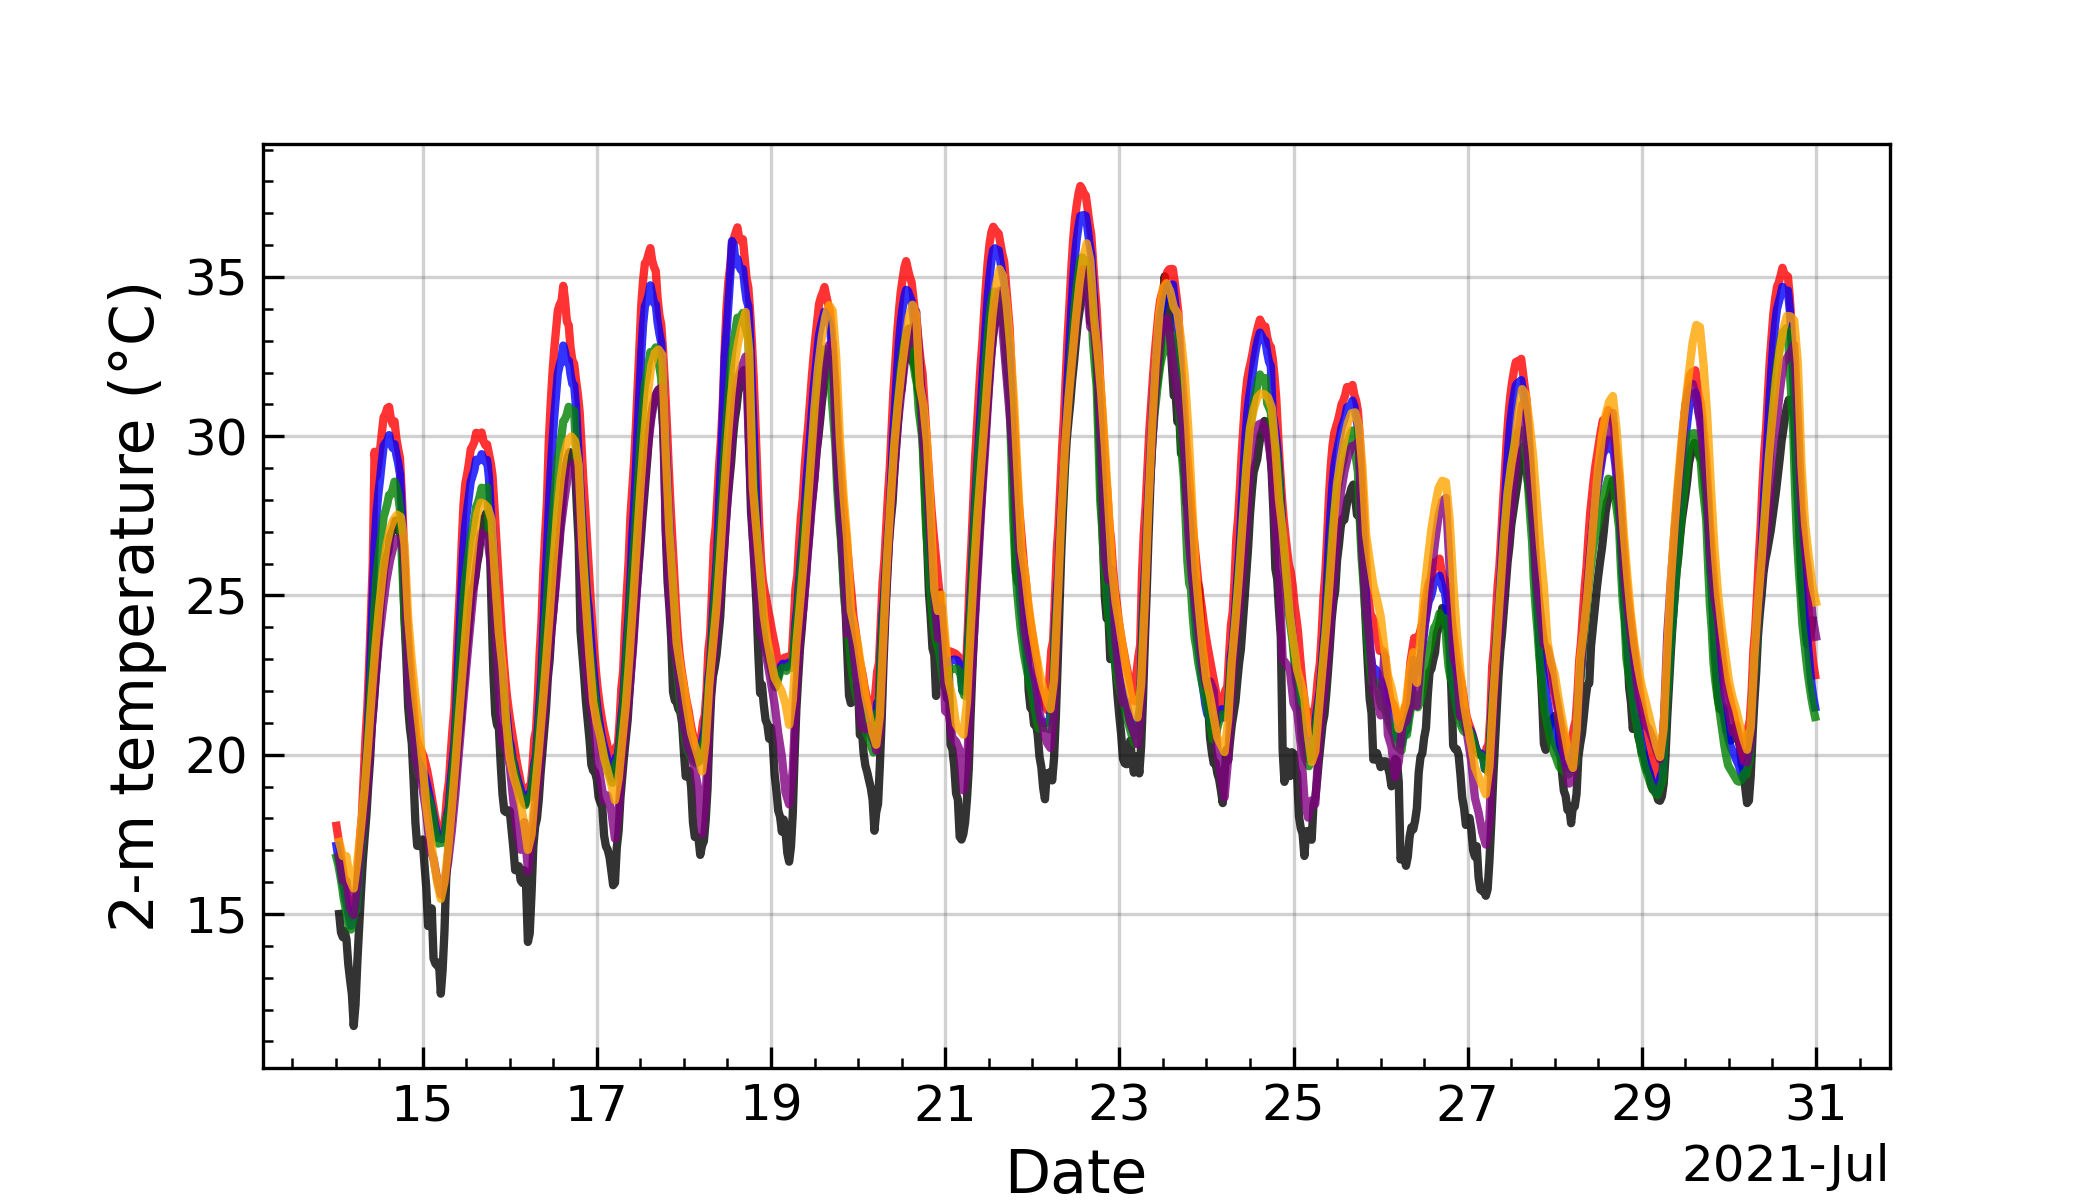
\includegraphics[width=\textwidth]{images/chap5/SOP_TS_DC/time_series_cendrosa_t2m.png}
        \end{subfigure} &
        \begin{subfigure}[t]{0.5\textwidth}
            \caption{}
            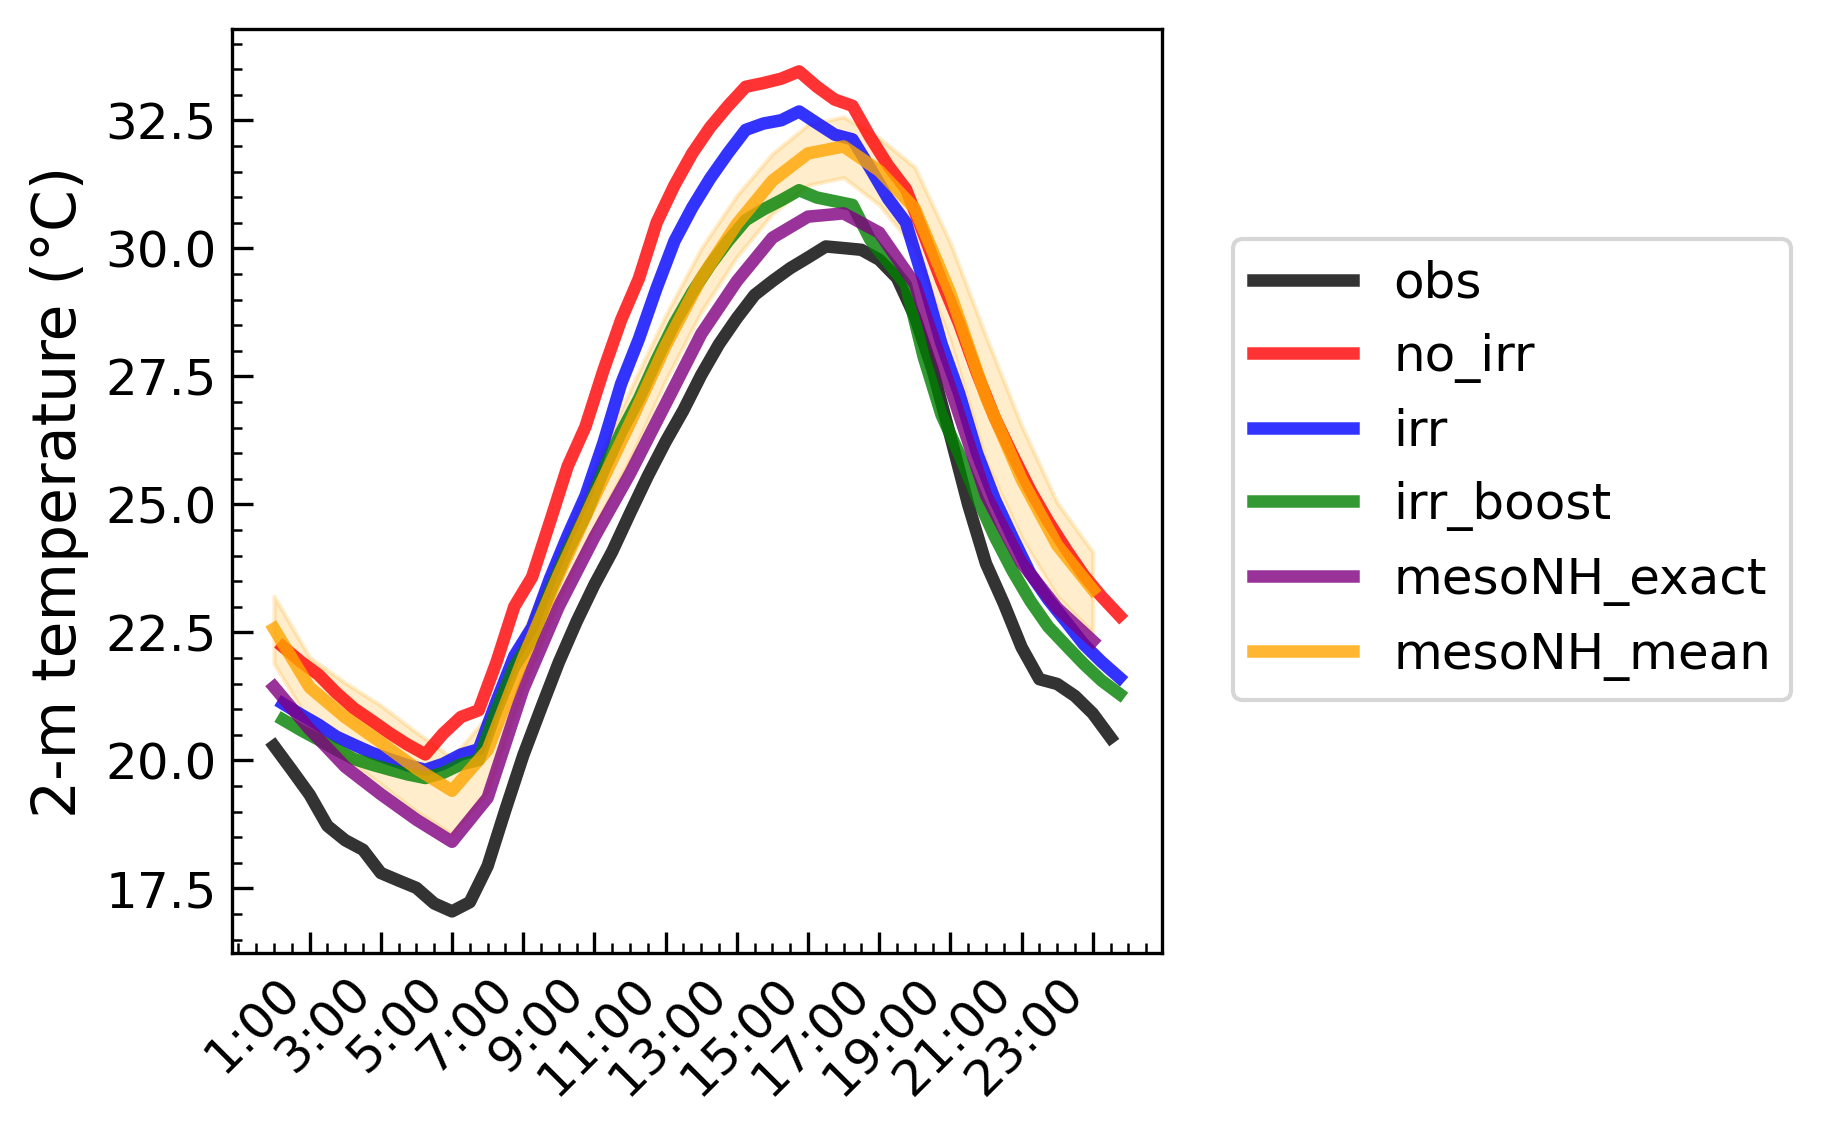
\includegraphics[width=\textwidth]{images/chap5/SOP_TS_DC/diurnal_cycle_cendrosa_t2m.png}
        \end{subfigure} \\
        
        % \vspace{1em} % Add vertical space between the rows
        \begin{subfigure}[t]{0.5\textwidth}
            \caption{}
            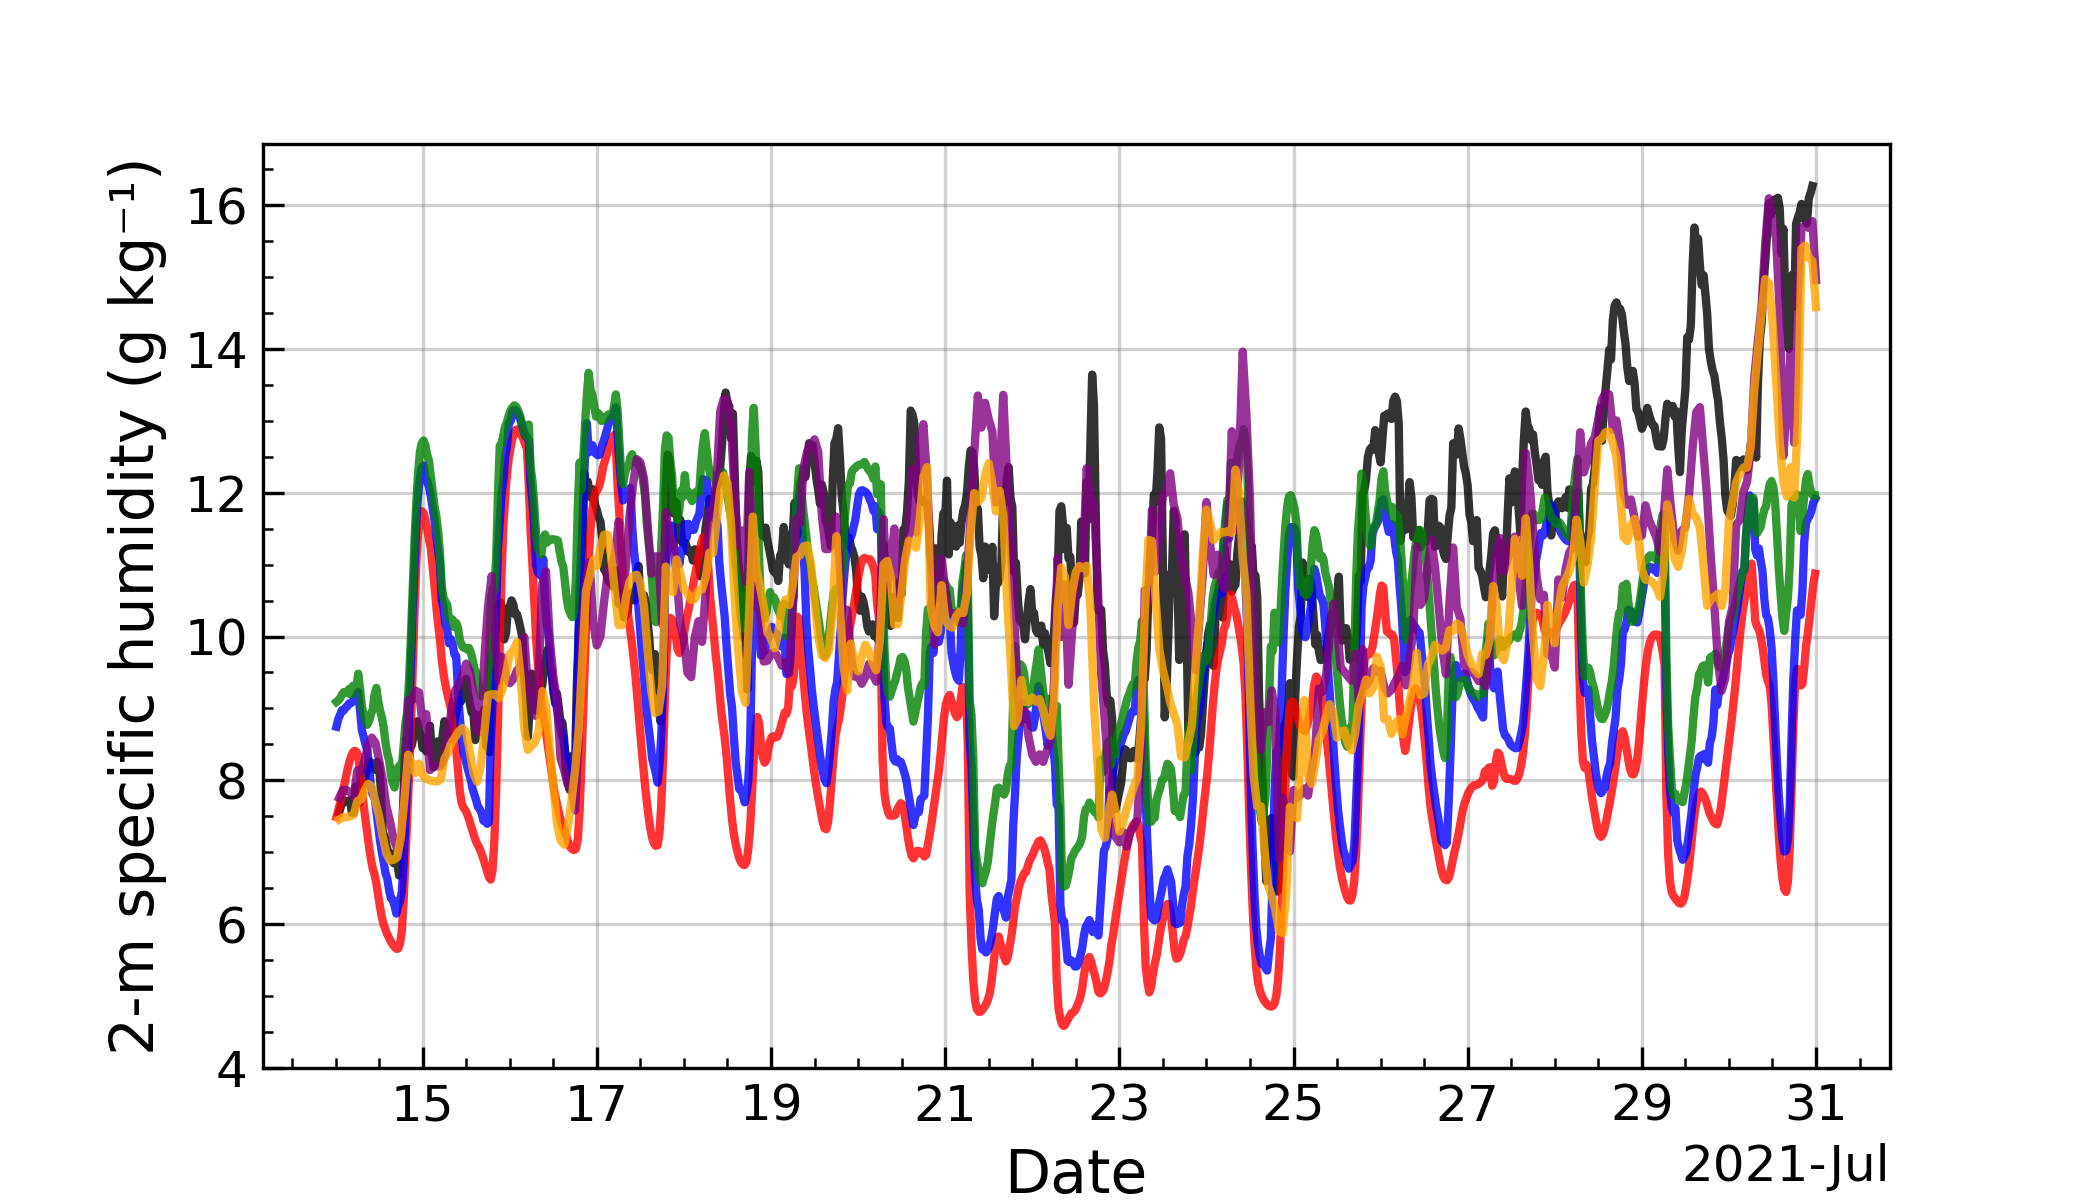
\includegraphics[width=\textwidth]{images/chap5/SOP_TS_DC/time_series_cendrosa_q2m.png}
        \end{subfigure} &
        \begin{subfigure}[t]{0.5\textwidth}
            \caption{}
            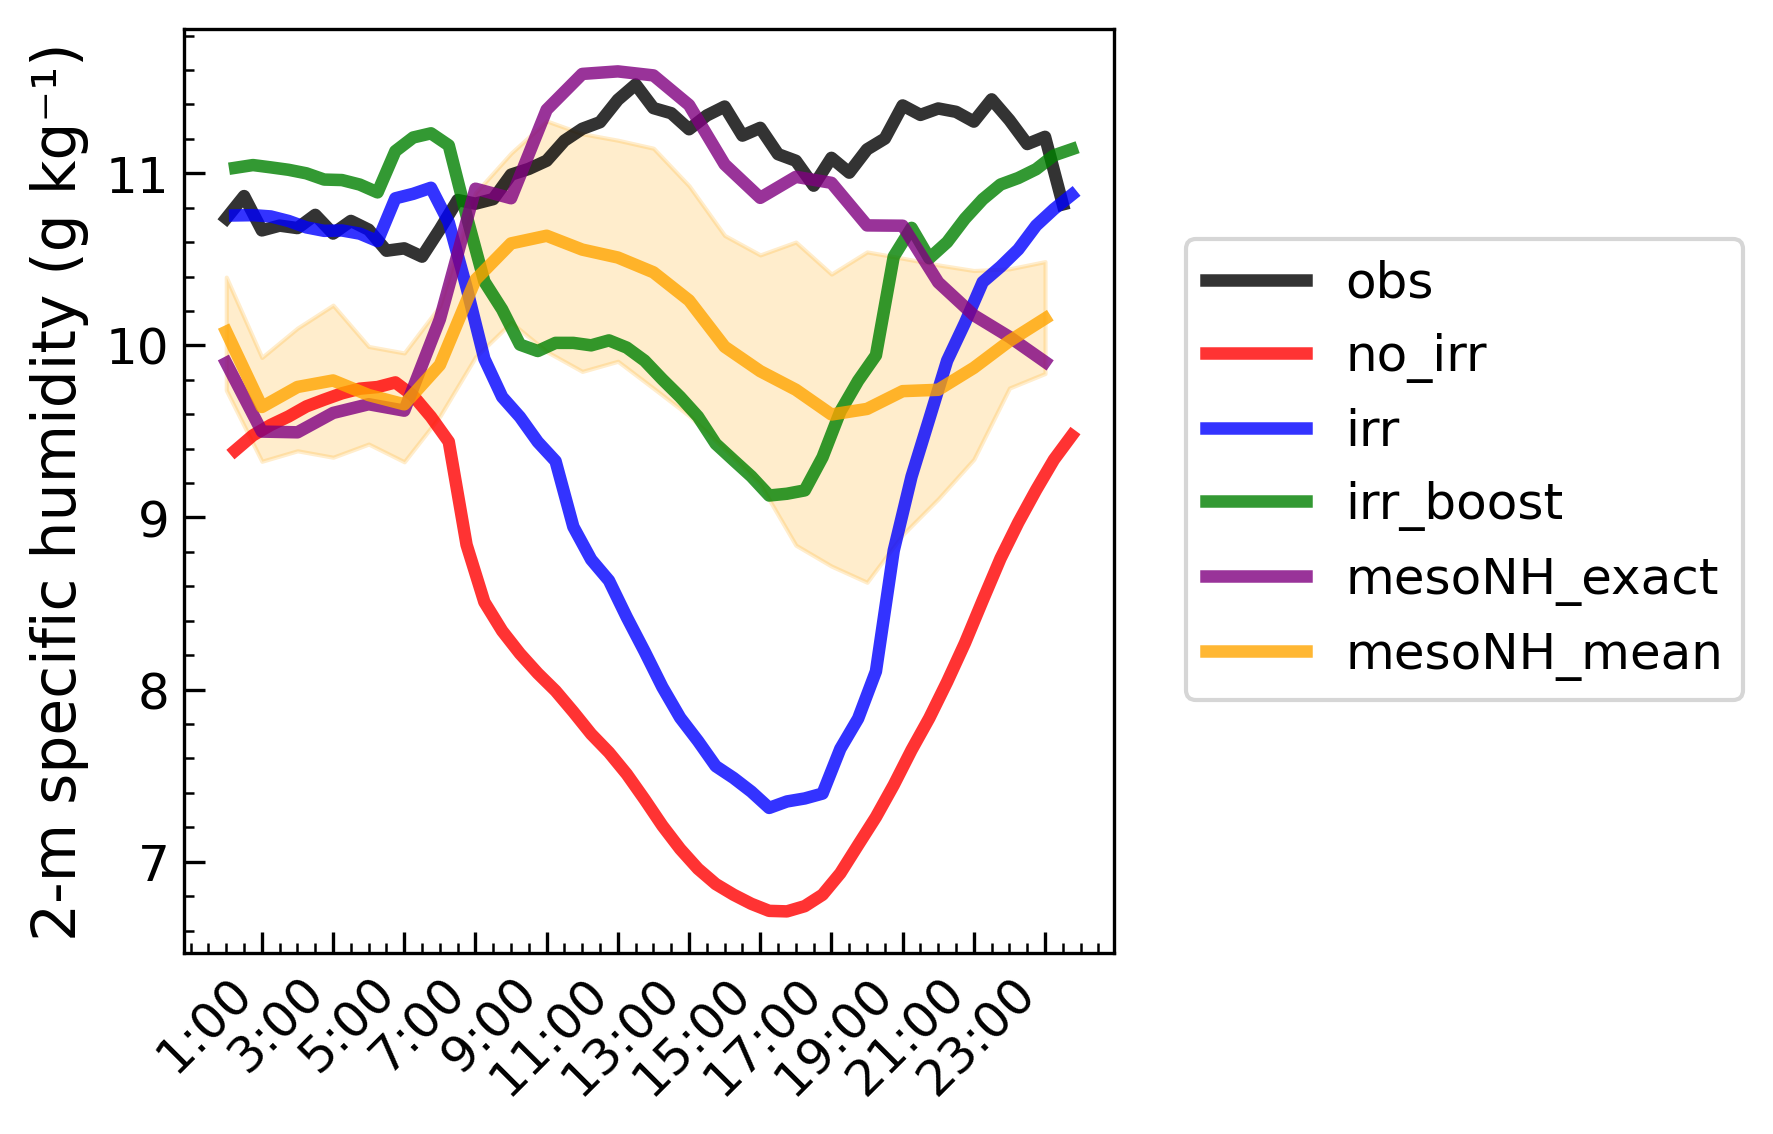
\includegraphics[width=\textwidth]{images/chap5/SOP_TS_DC/diurnal_cycle_cendrosa_q2m.png}
        \end{subfigure} \\
    \end{tabular}
    \caption{Time series and mean diurnal cycle of surface turbulent fluxes at La Cendrosa (irrigated site), July 14-30 2021.}
    \label{fig:cendrosa_surfacevars}
\end{figure}
%Fig : Els Plans turbulent fluxes + t2m, q2m
\begin{figure}[hbtp]
    \centering
    \begin{tabular}{cc}
        \begin{subfigure}[t]{0.5\textwidth}
            \caption{}
            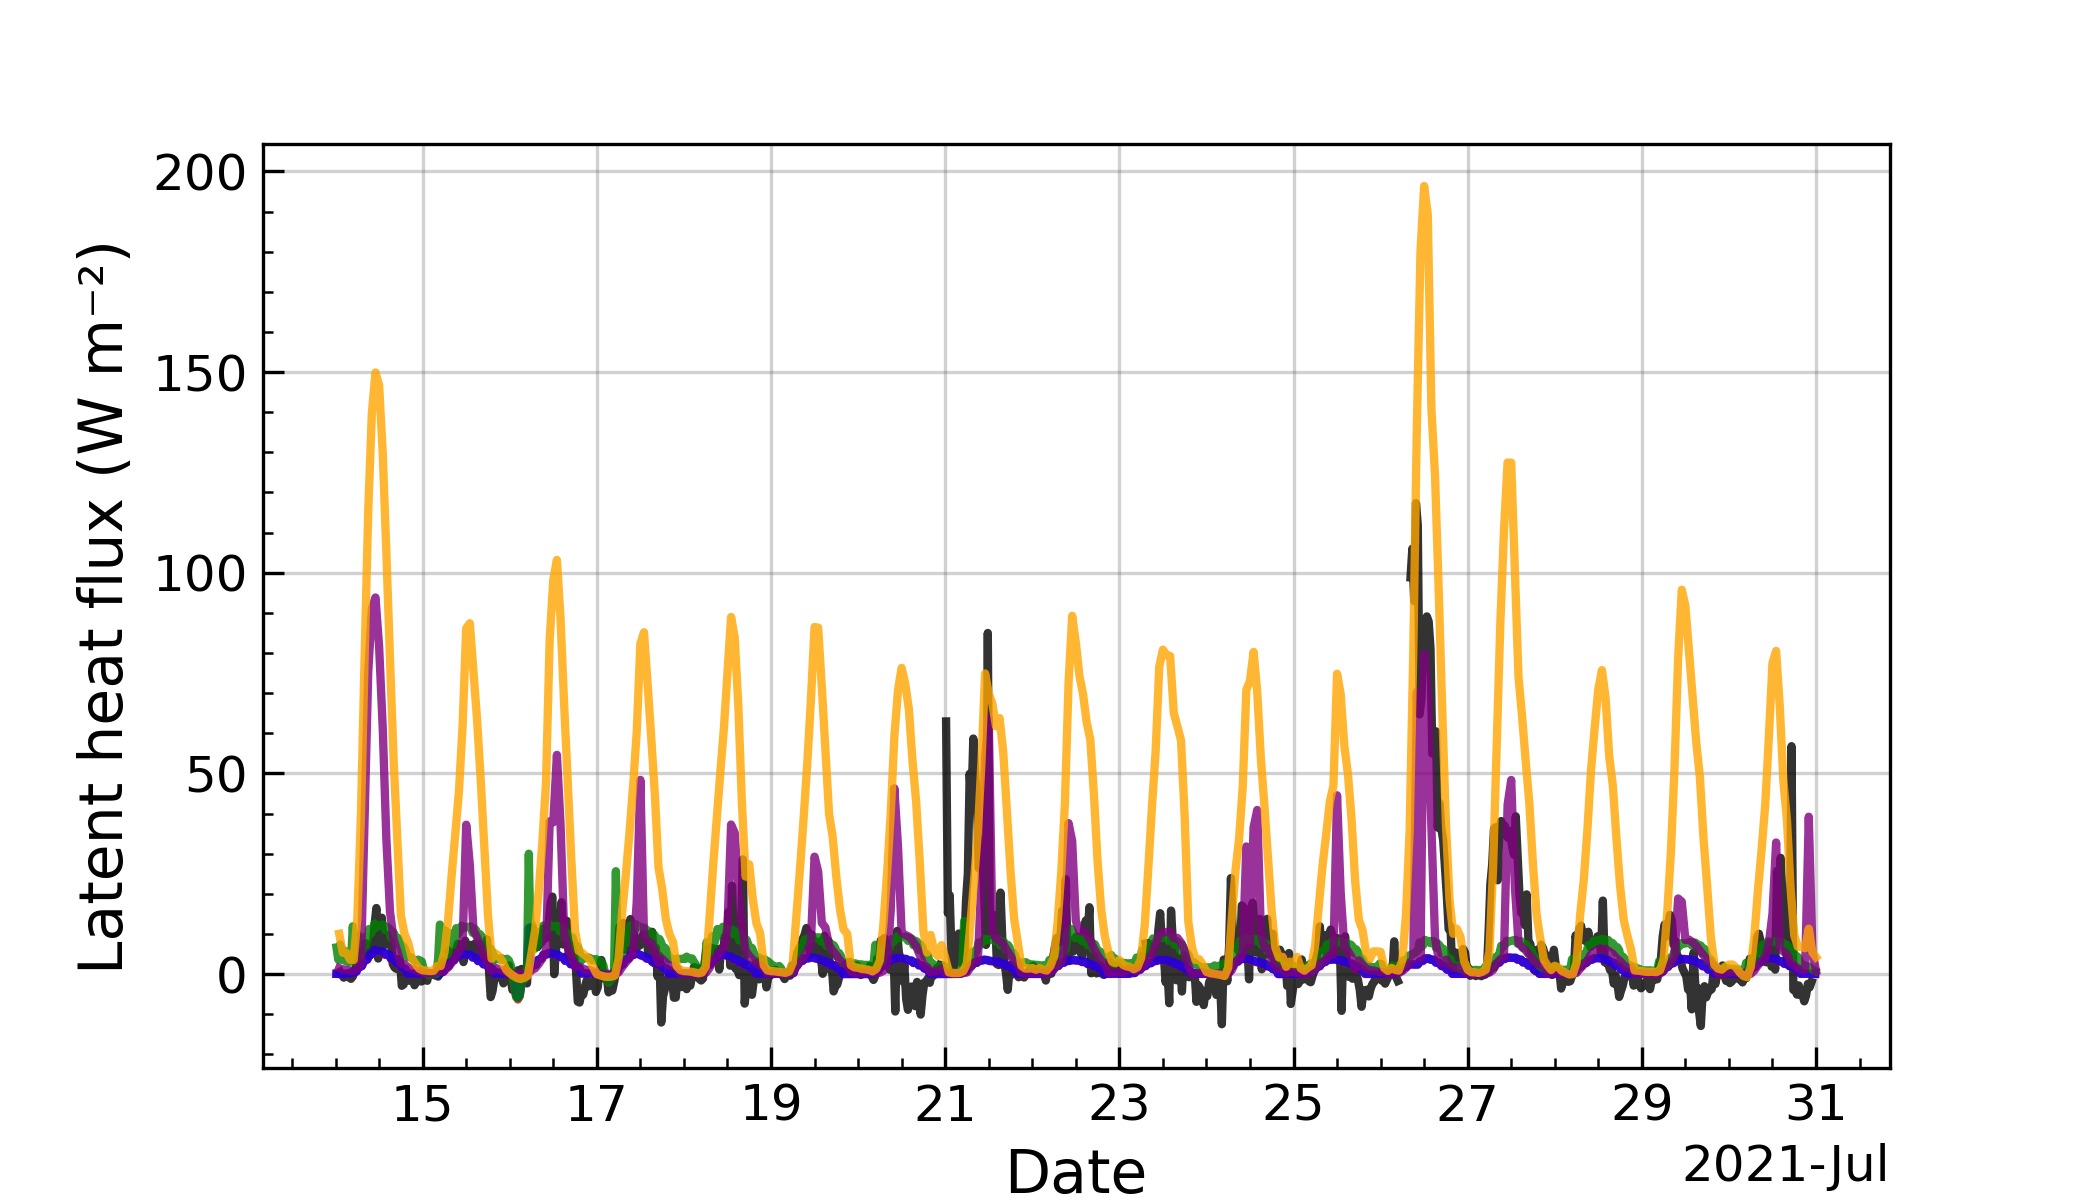
\includegraphics[width=\textwidth]{images/chap5/SOP_TS_DC/time_series_elsplans_flat.png}
        \end{subfigure} &
        \begin{subfigure}[t]{0.5\textwidth}
            \caption{}
            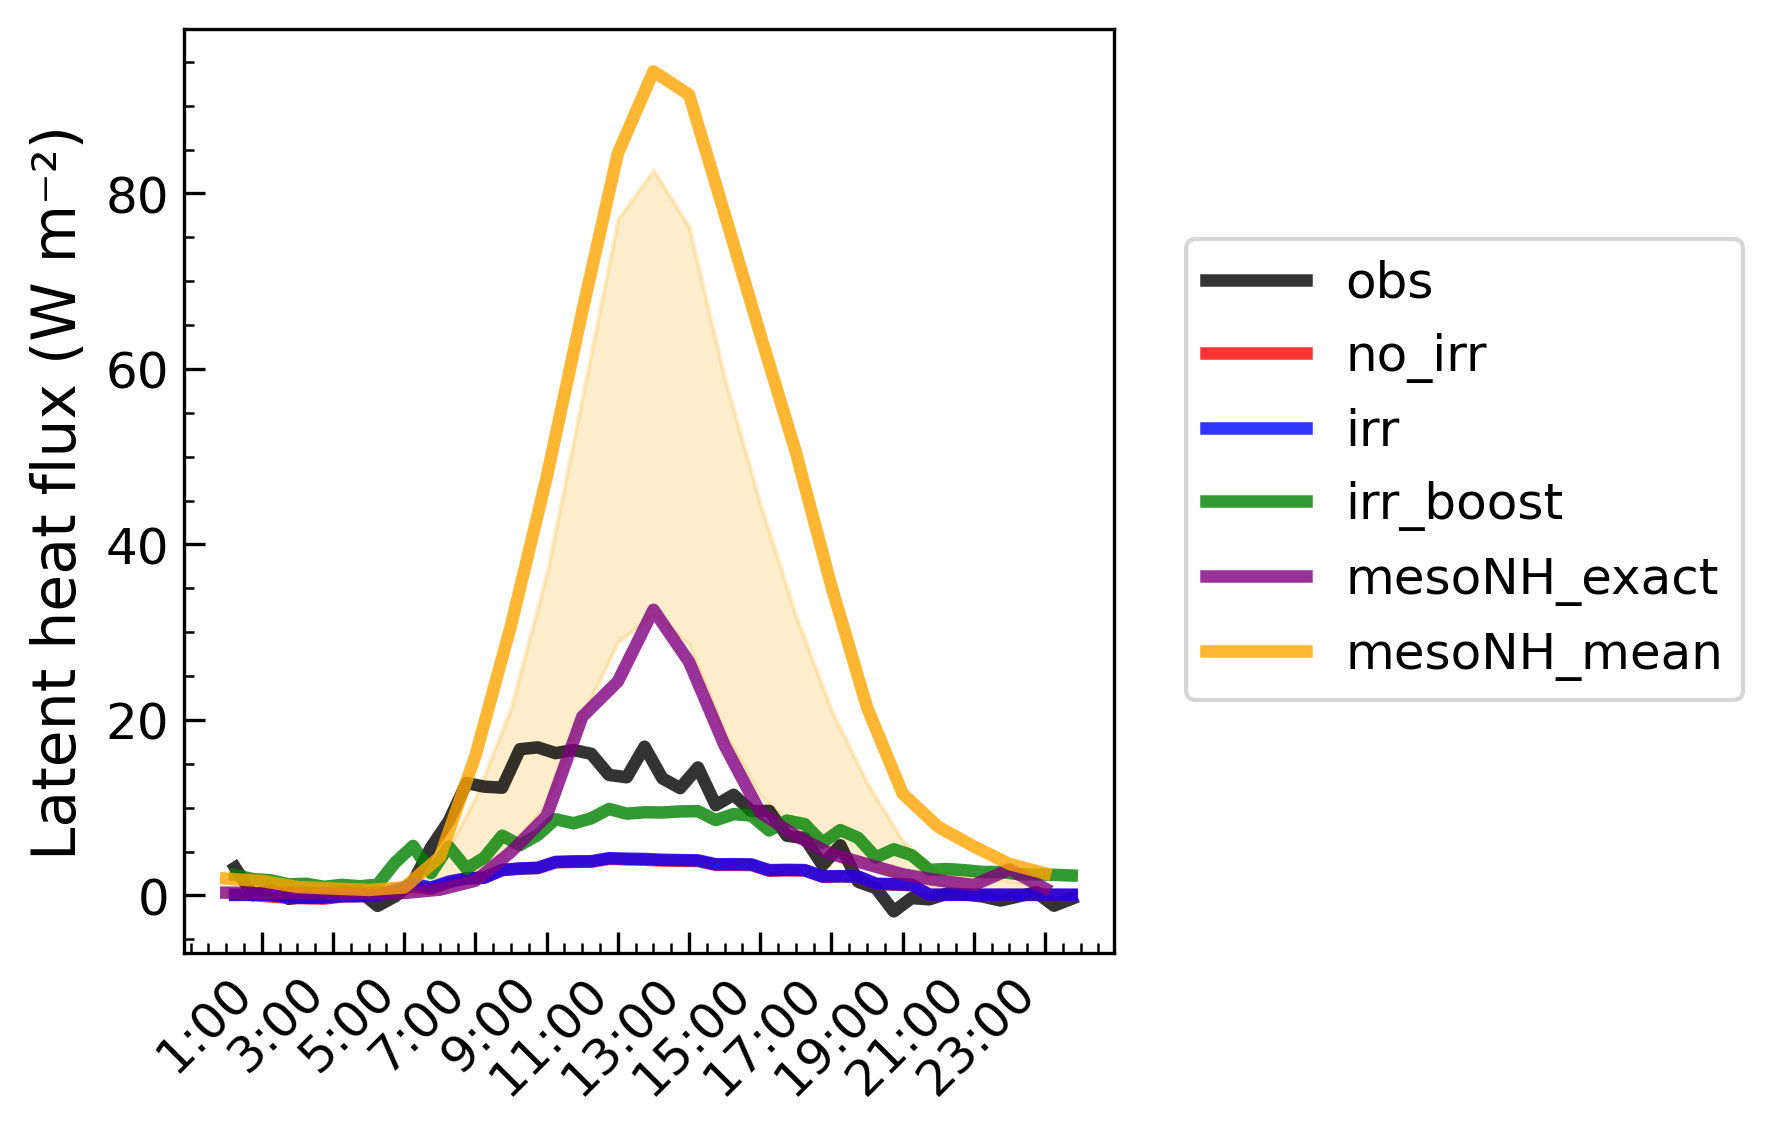
\includegraphics[width=\textwidth]{images/chap5/SOP_TS_DC/diurnal_cycle_elsplans_flat.png}
        \end{subfigure} \\
        
        % \vspace{1em} % Add vertical space between the rows
        \begin{subfigure}[t]{0.5\textwidth}
            \caption{}
            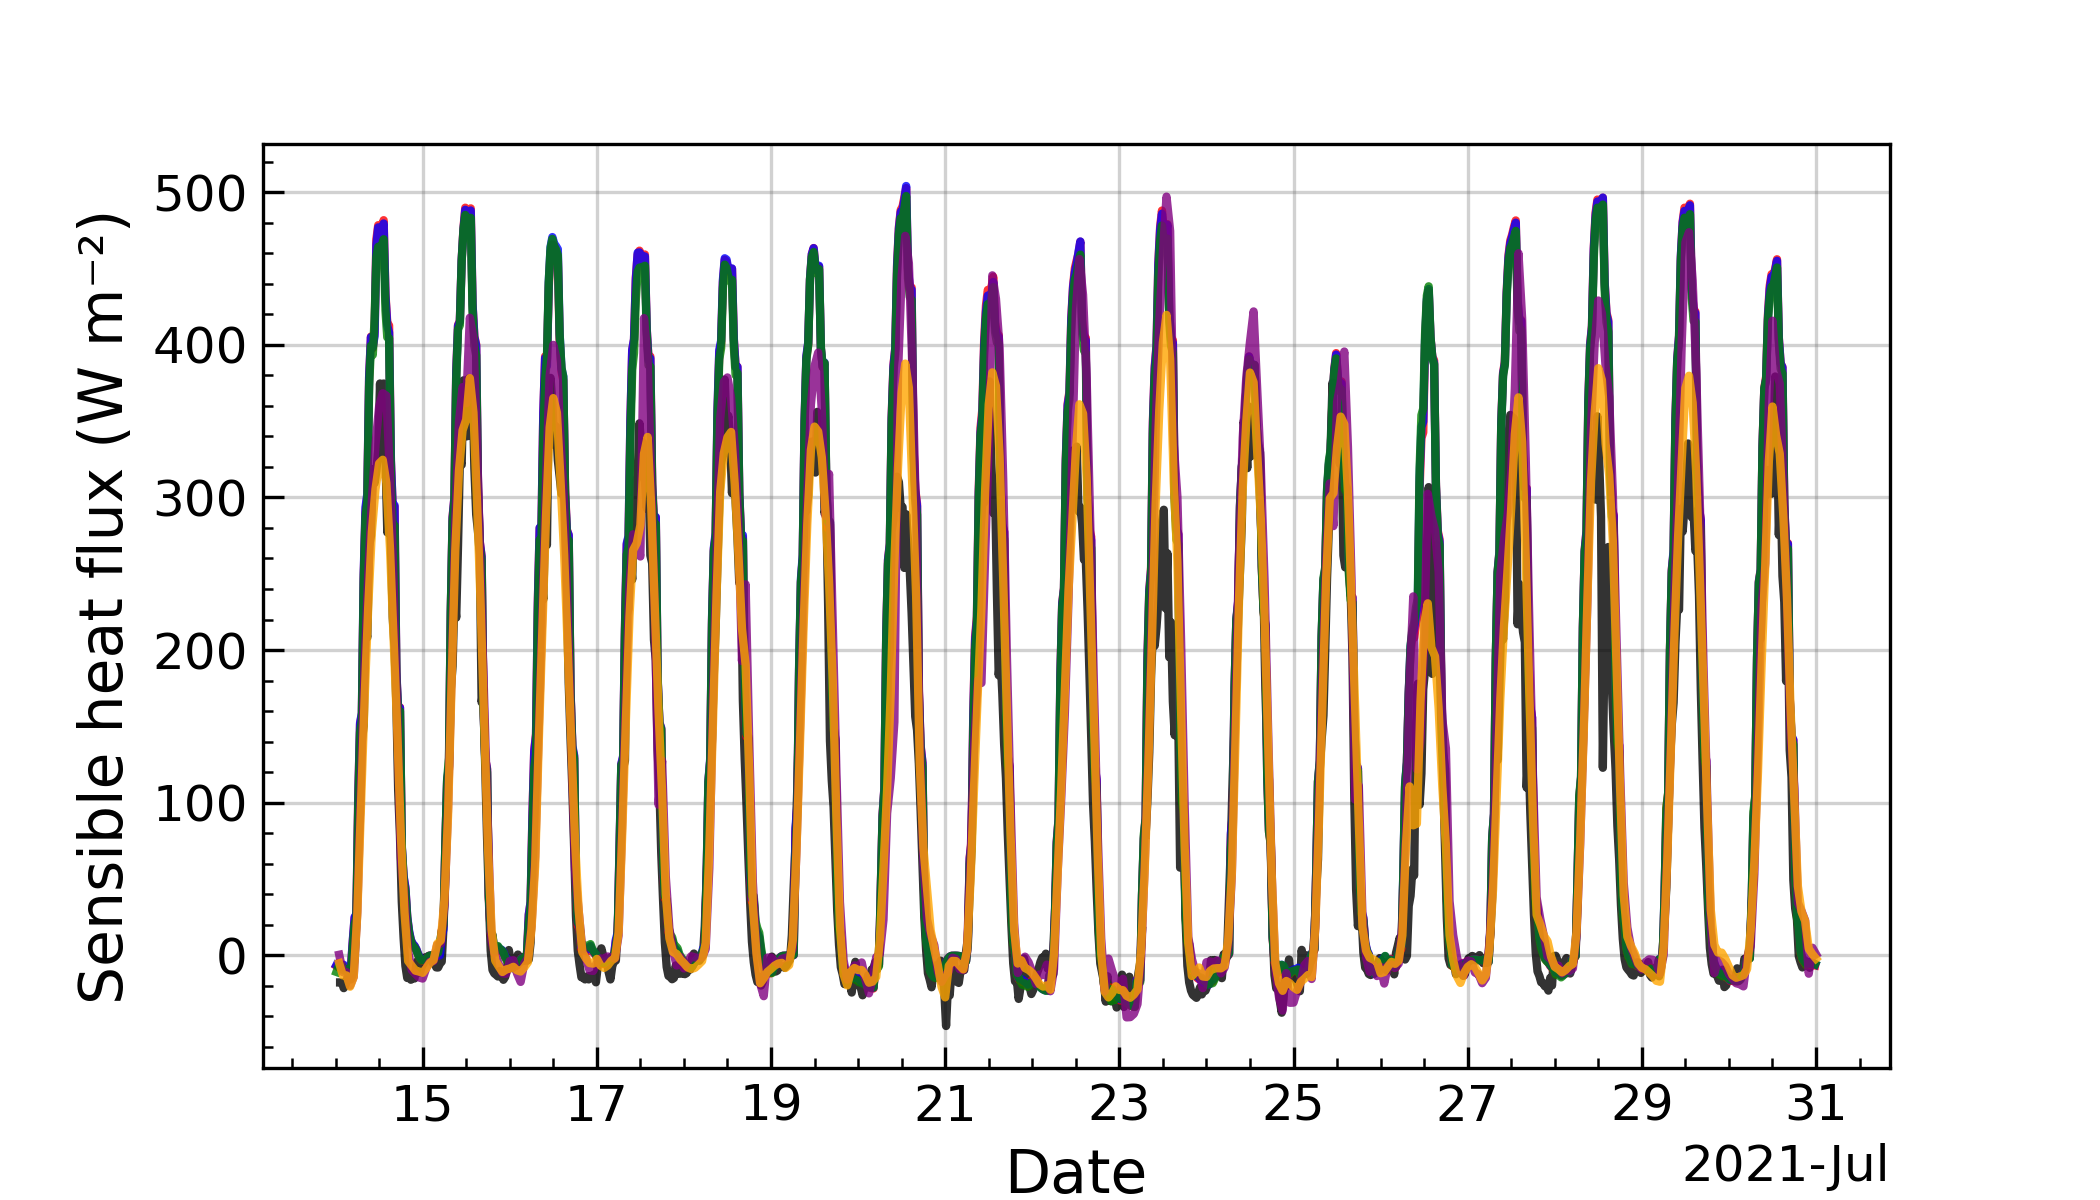
\includegraphics[width=\textwidth]{images/chap5/SOP_TS_DC/time_series_elsplans_sens.png}
        \end{subfigure} &
        \begin{subfigure}[t]{0.5\textwidth}
            \caption{}
            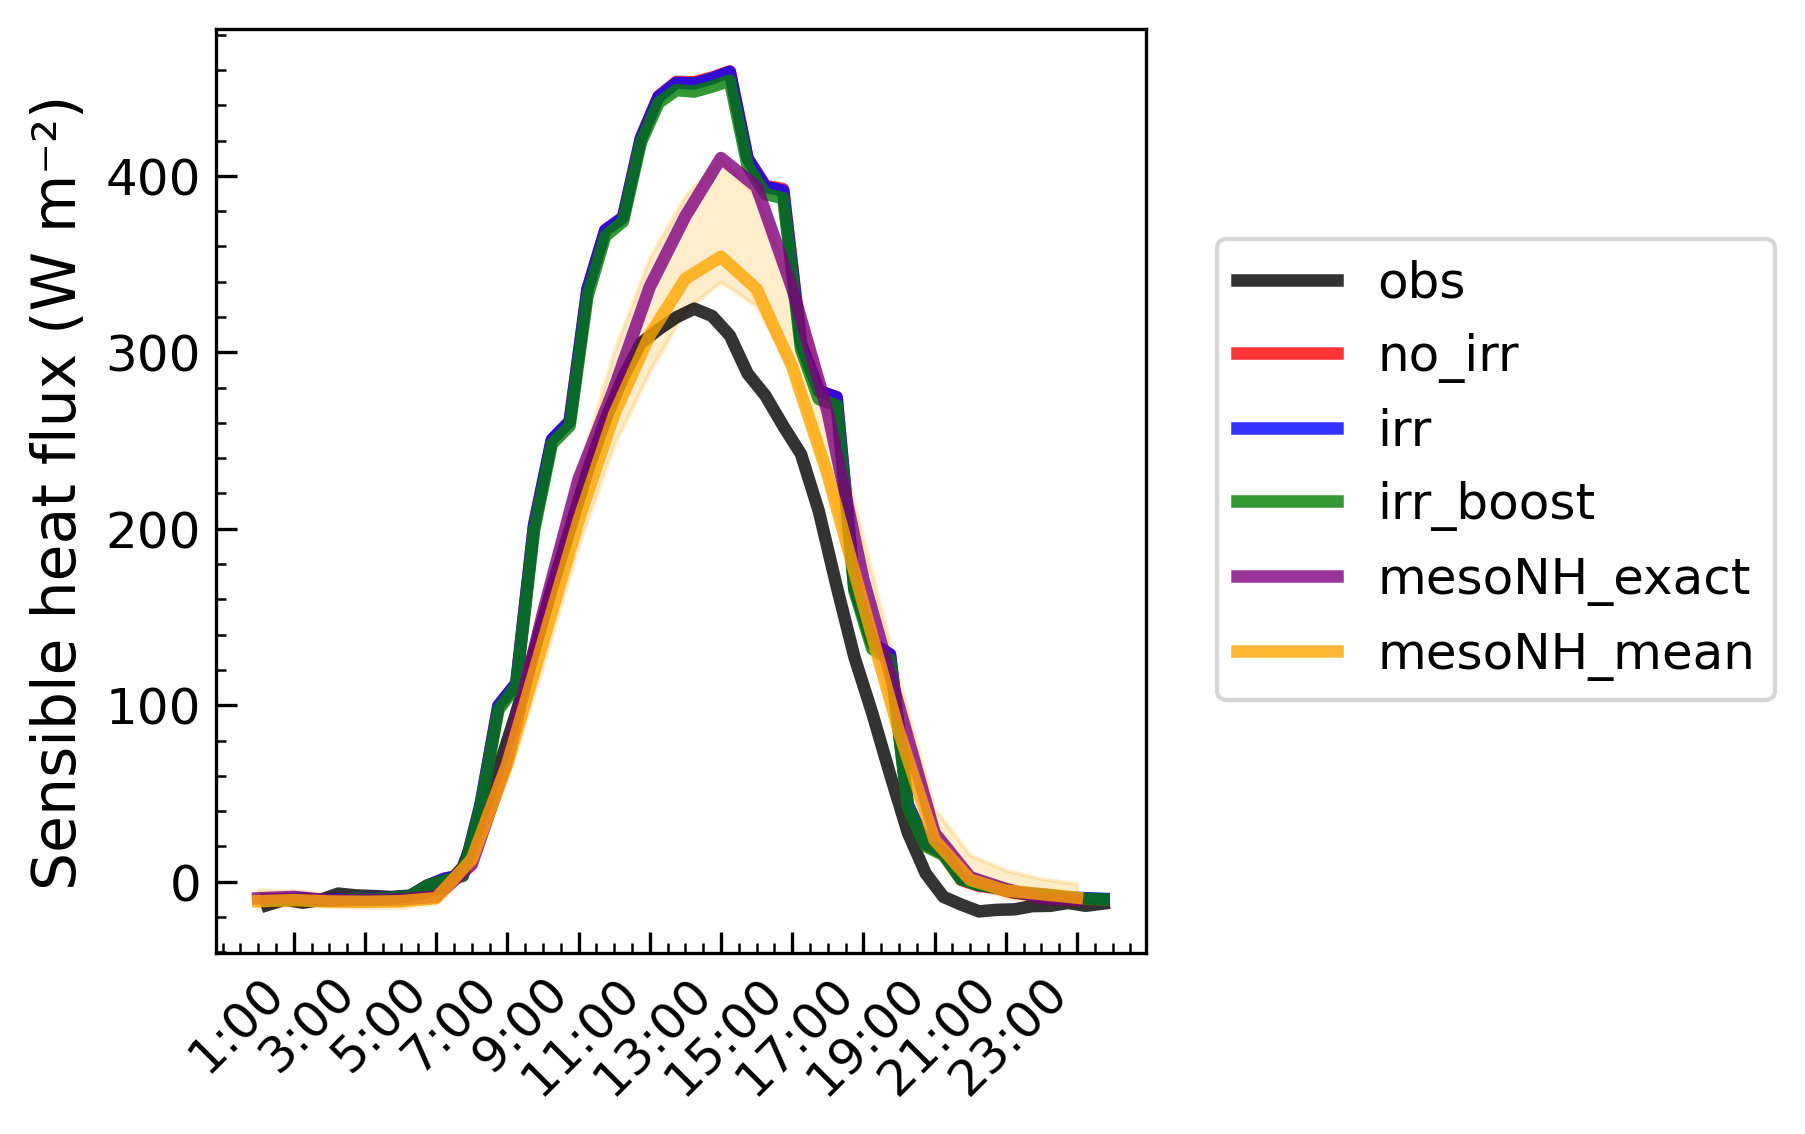
\includegraphics[width=\textwidth]{images/chap5/SOP_TS_DC/diurnal_cycle_elsplans_sens.png}
        \end{subfigure} \\

        \begin{subfigure}[t]{0.5\textwidth}
            \caption{}
            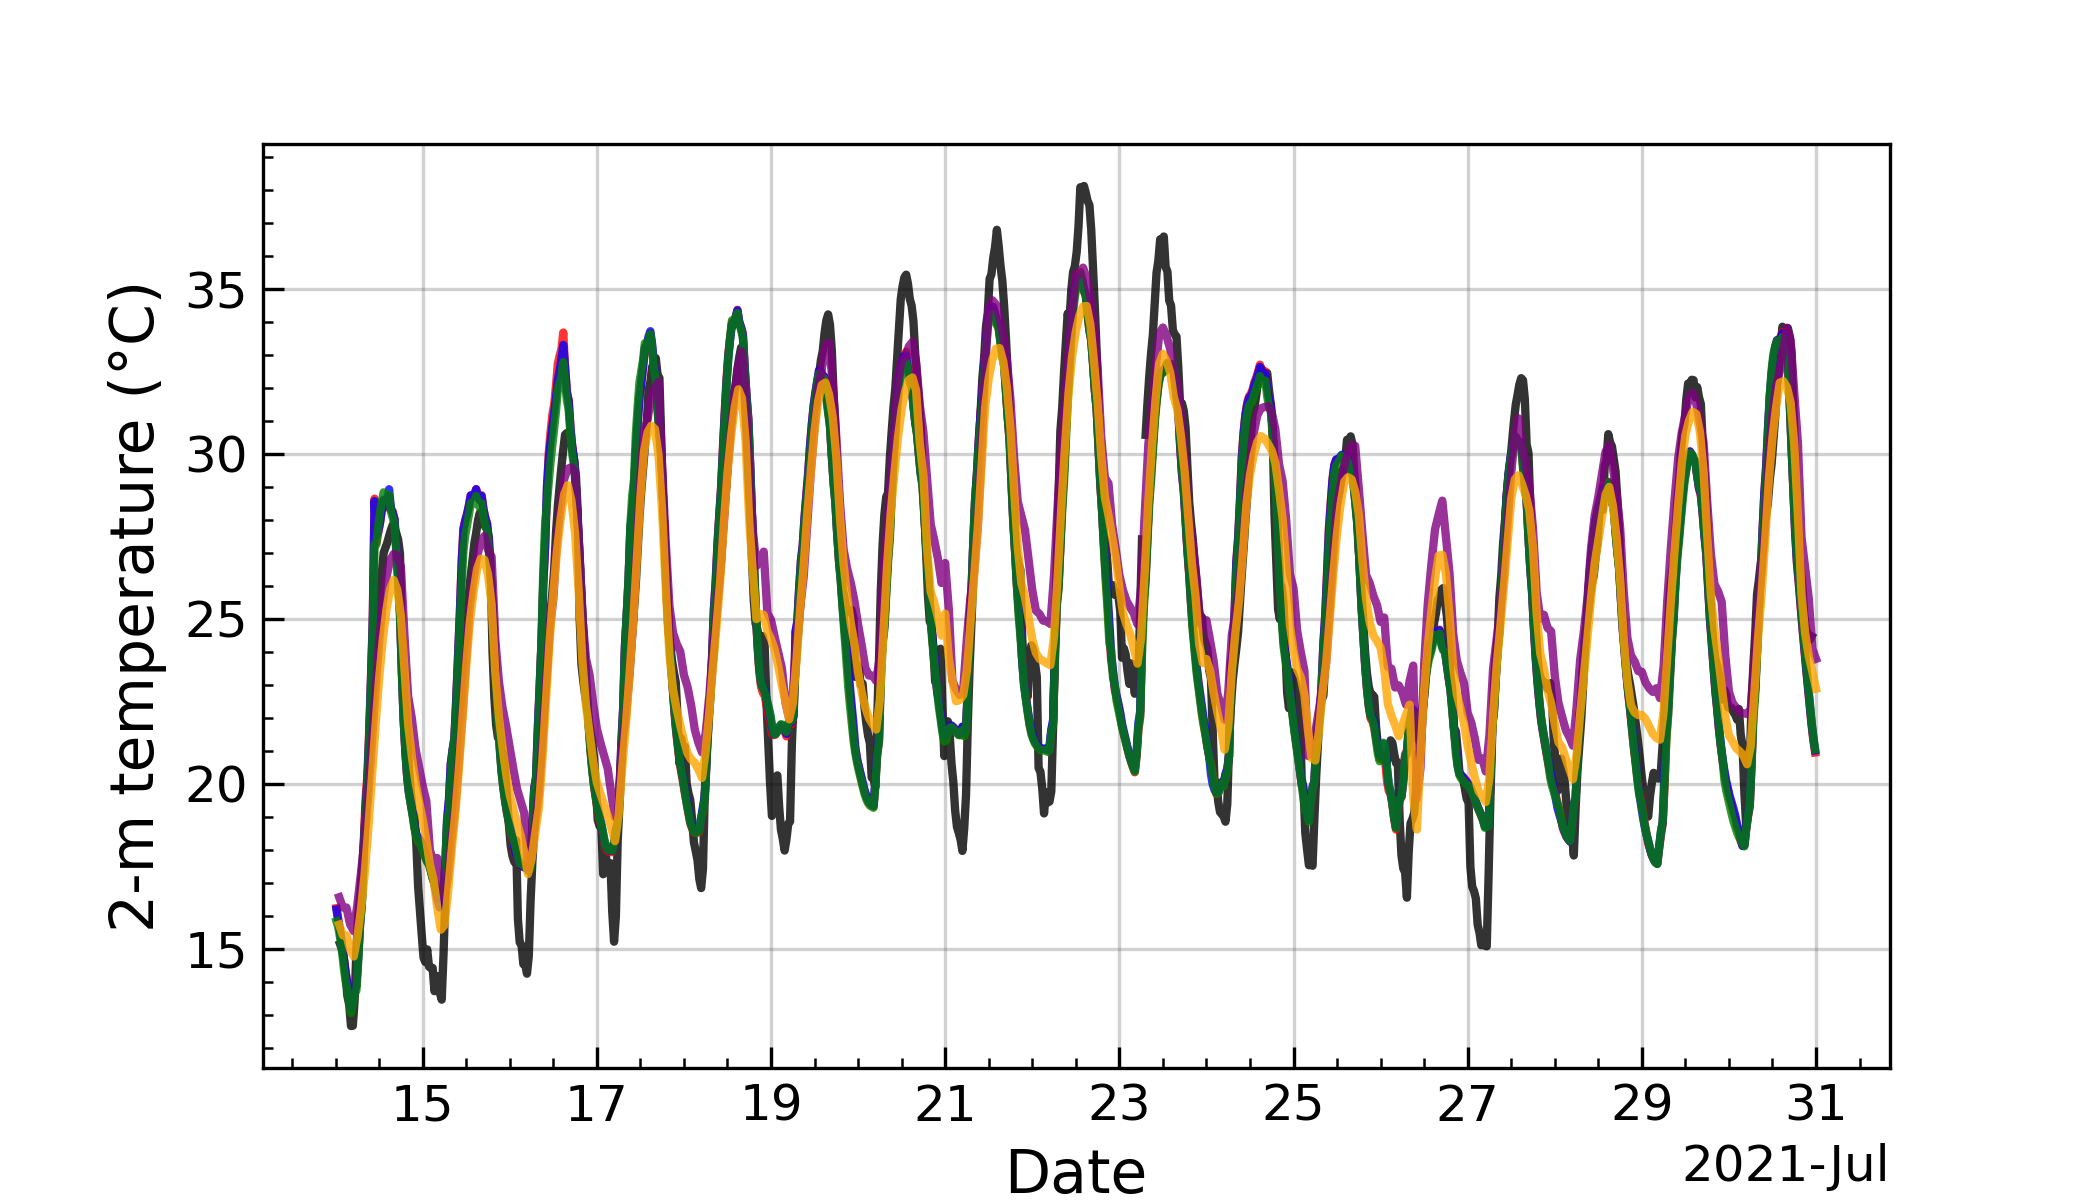
\includegraphics[width=\textwidth]{images/chap5/SOP_TS_DC/time_series_elsplans_t2m.png}
        \end{subfigure} &
        \begin{subfigure}[t]{0.5\textwidth}
            \caption{}
            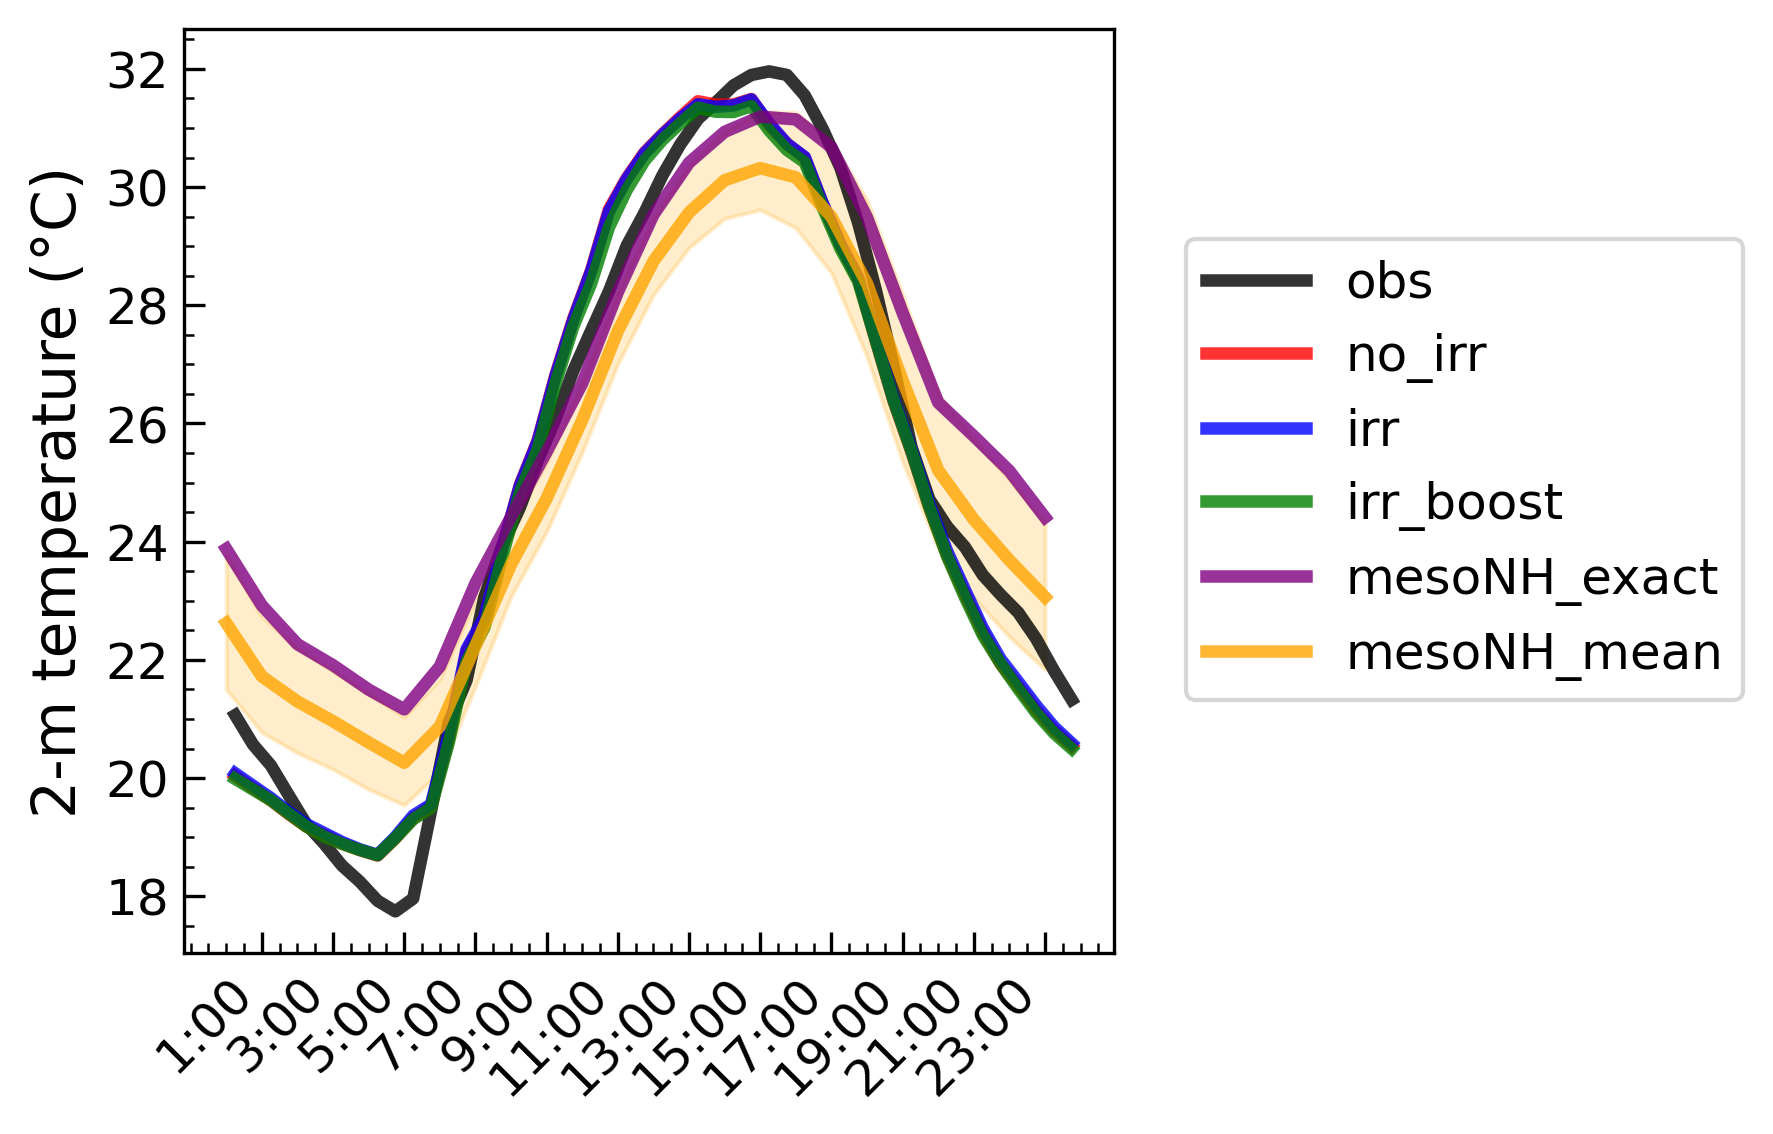
\includegraphics[width=\textwidth]{images/chap5/SOP_TS_DC/diurnal_cycle_elsplans_t2m.png}
        \end{subfigure} \\
        
        % \vspace{1em} % Add vertical space between the rows
        \begin{subfigure}[t]{0.5\textwidth}
            \caption{}
            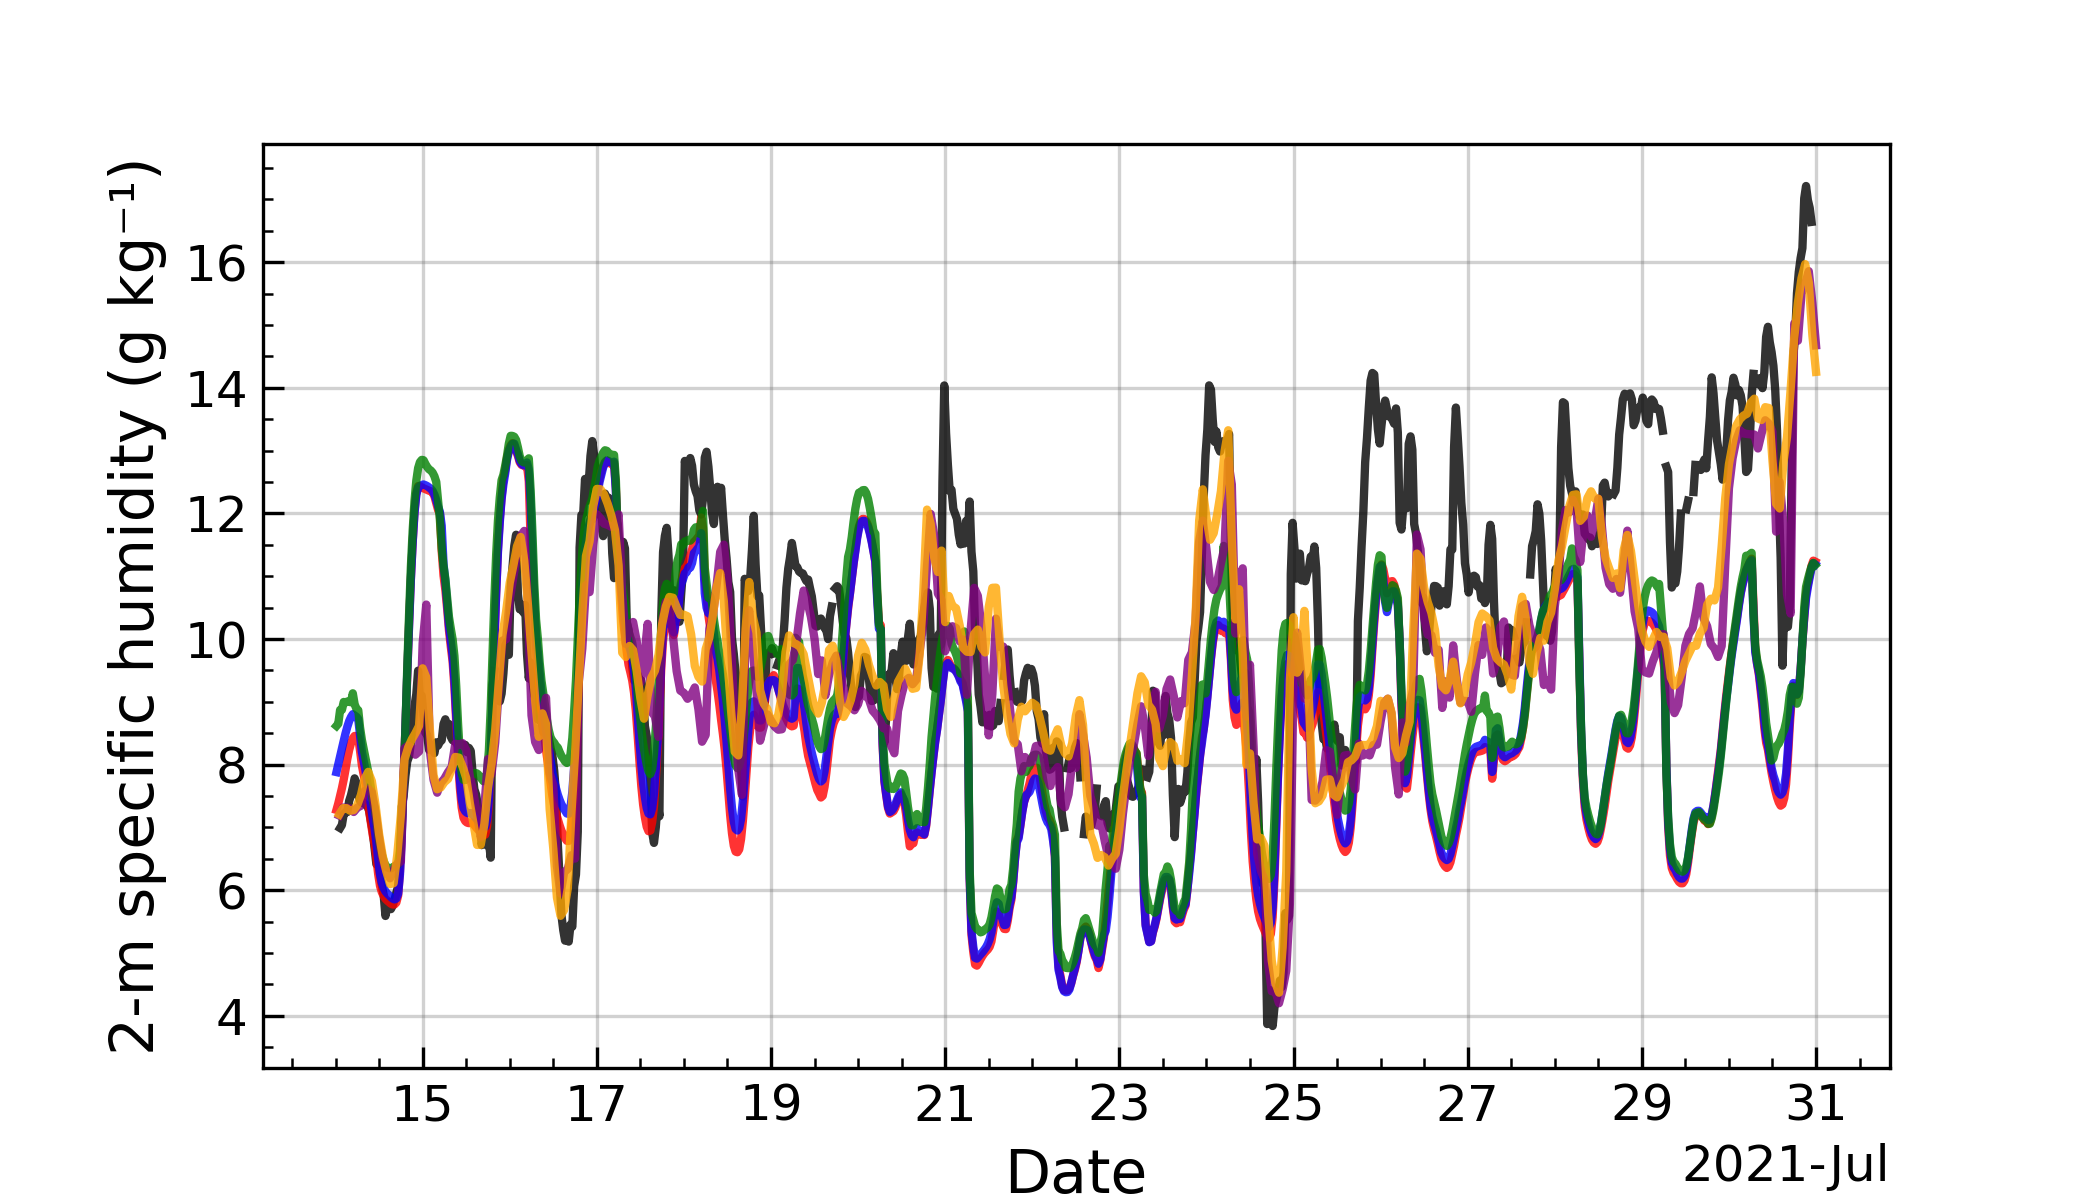
\includegraphics[width=\textwidth]{images/chap5/SOP_TS_DC/time_series_elsplans_q2m.png}
        \end{subfigure} &
        \begin{subfigure}[t]{0.5\textwidth}
            \caption{}
            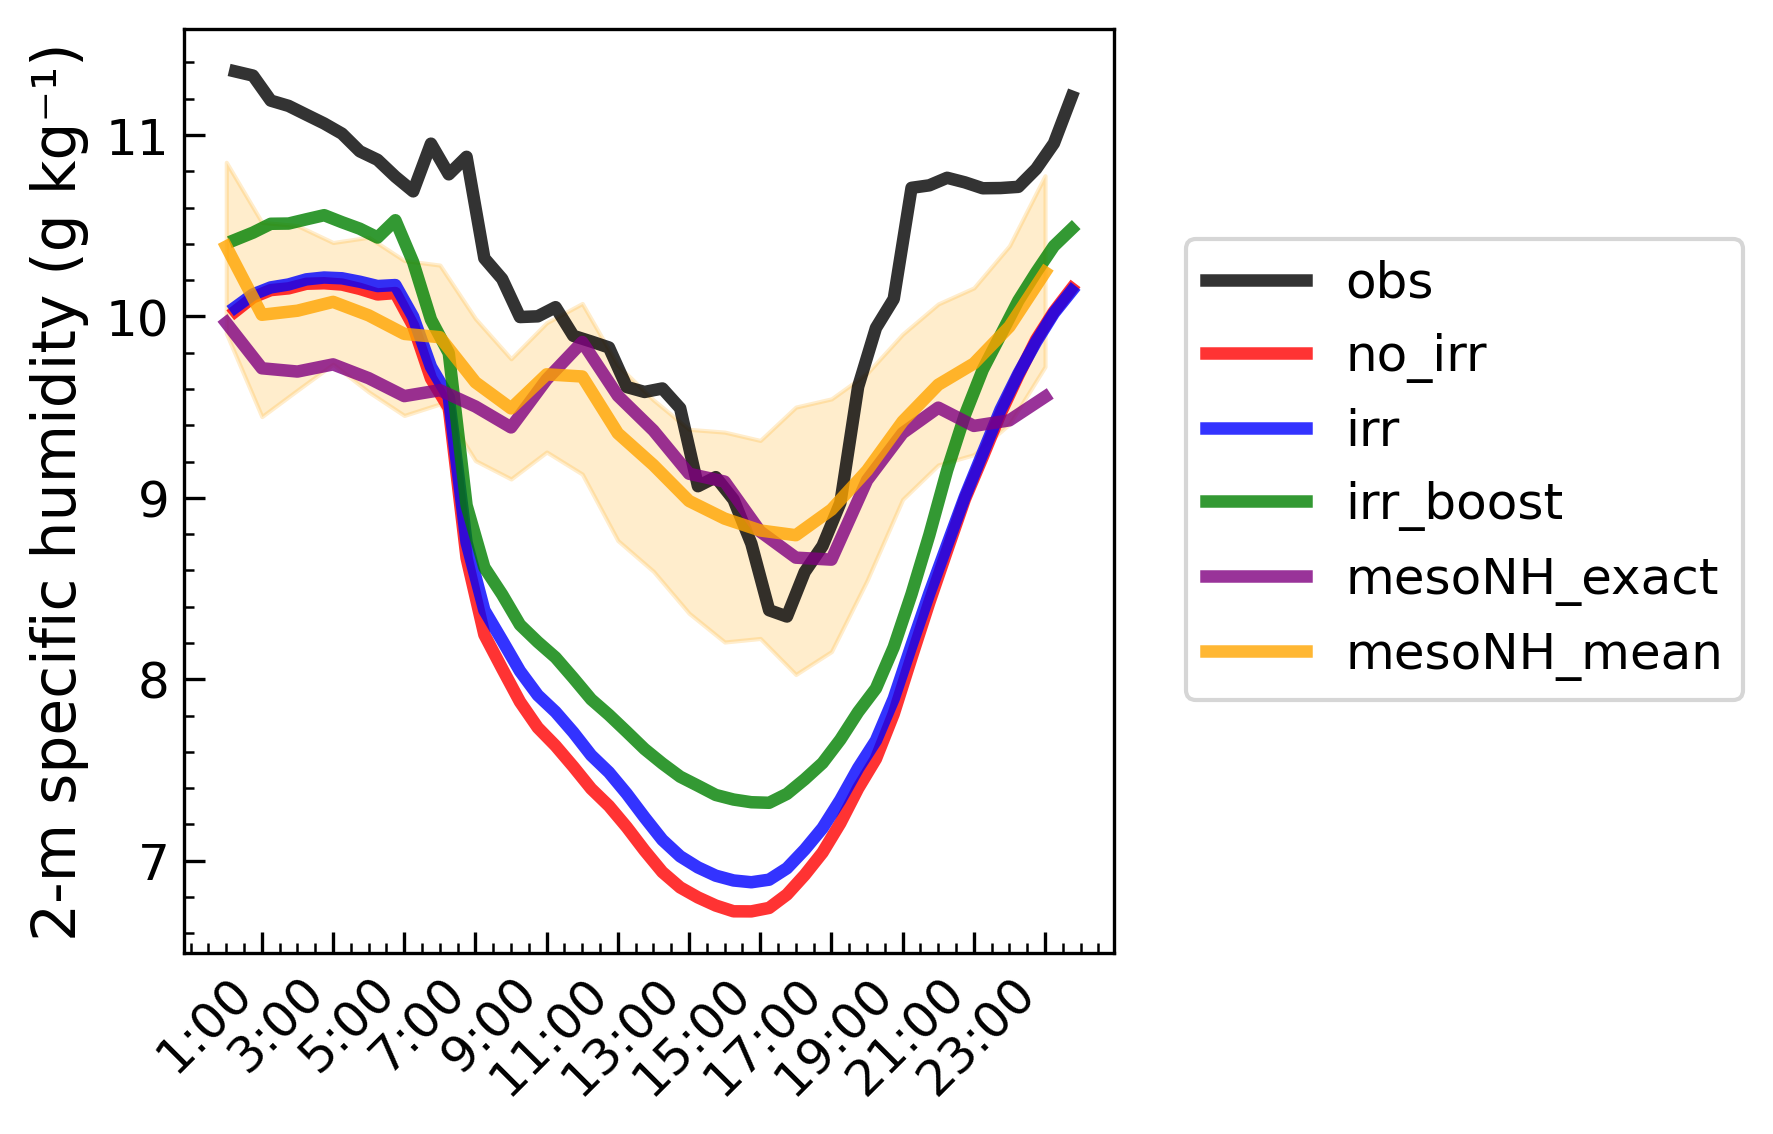
\includegraphics[width=\textwidth]{images/chap5/SOP_TS_DC/diurnal_cycle_elsplans_q2m.png}
        \end{subfigure} \\
    \end{tabular}
    \caption{Time series and mean diurnal cycle of surface turbulent fluxes at Els Plans (rainfed site), July 14-30 2021.}
    \label{fig:elsplans_surfacevars}
\end{figure}
%Fig : Wind on both sites
\begin{figure}[hbtp]
    \centering
    \begin{tabular}{cc}
        \begin{subfigure}[t]{0.5\textwidth}
            \caption{}
            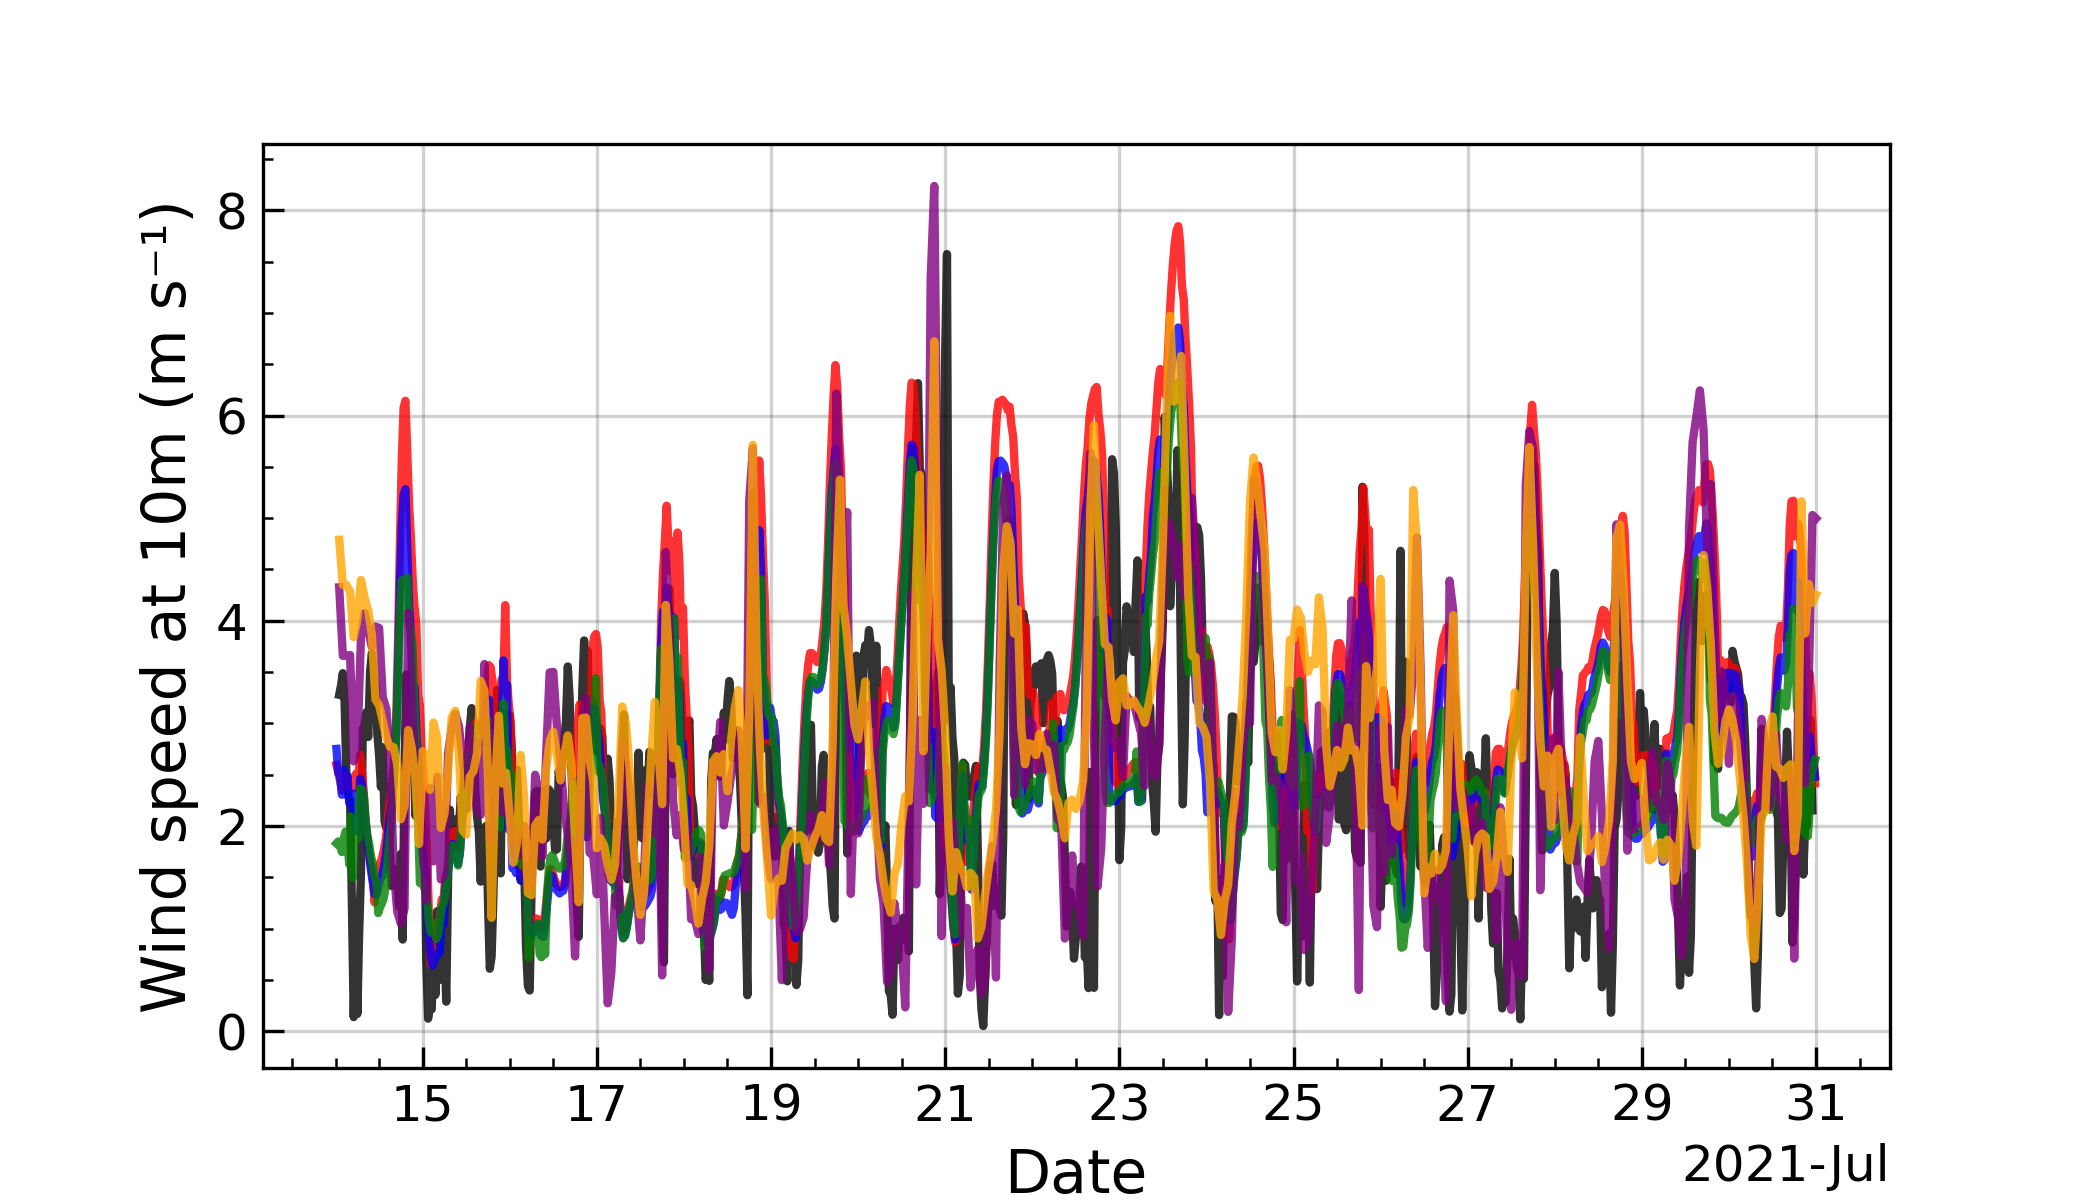
\includegraphics[width=\textwidth]{images/chap5/SOP_TS_DC/time_series_cendrosa_wind_speed_10m.png}
        \end{subfigure} &
        \begin{subfigure}[t]{0.5\textwidth}
            \caption{}
            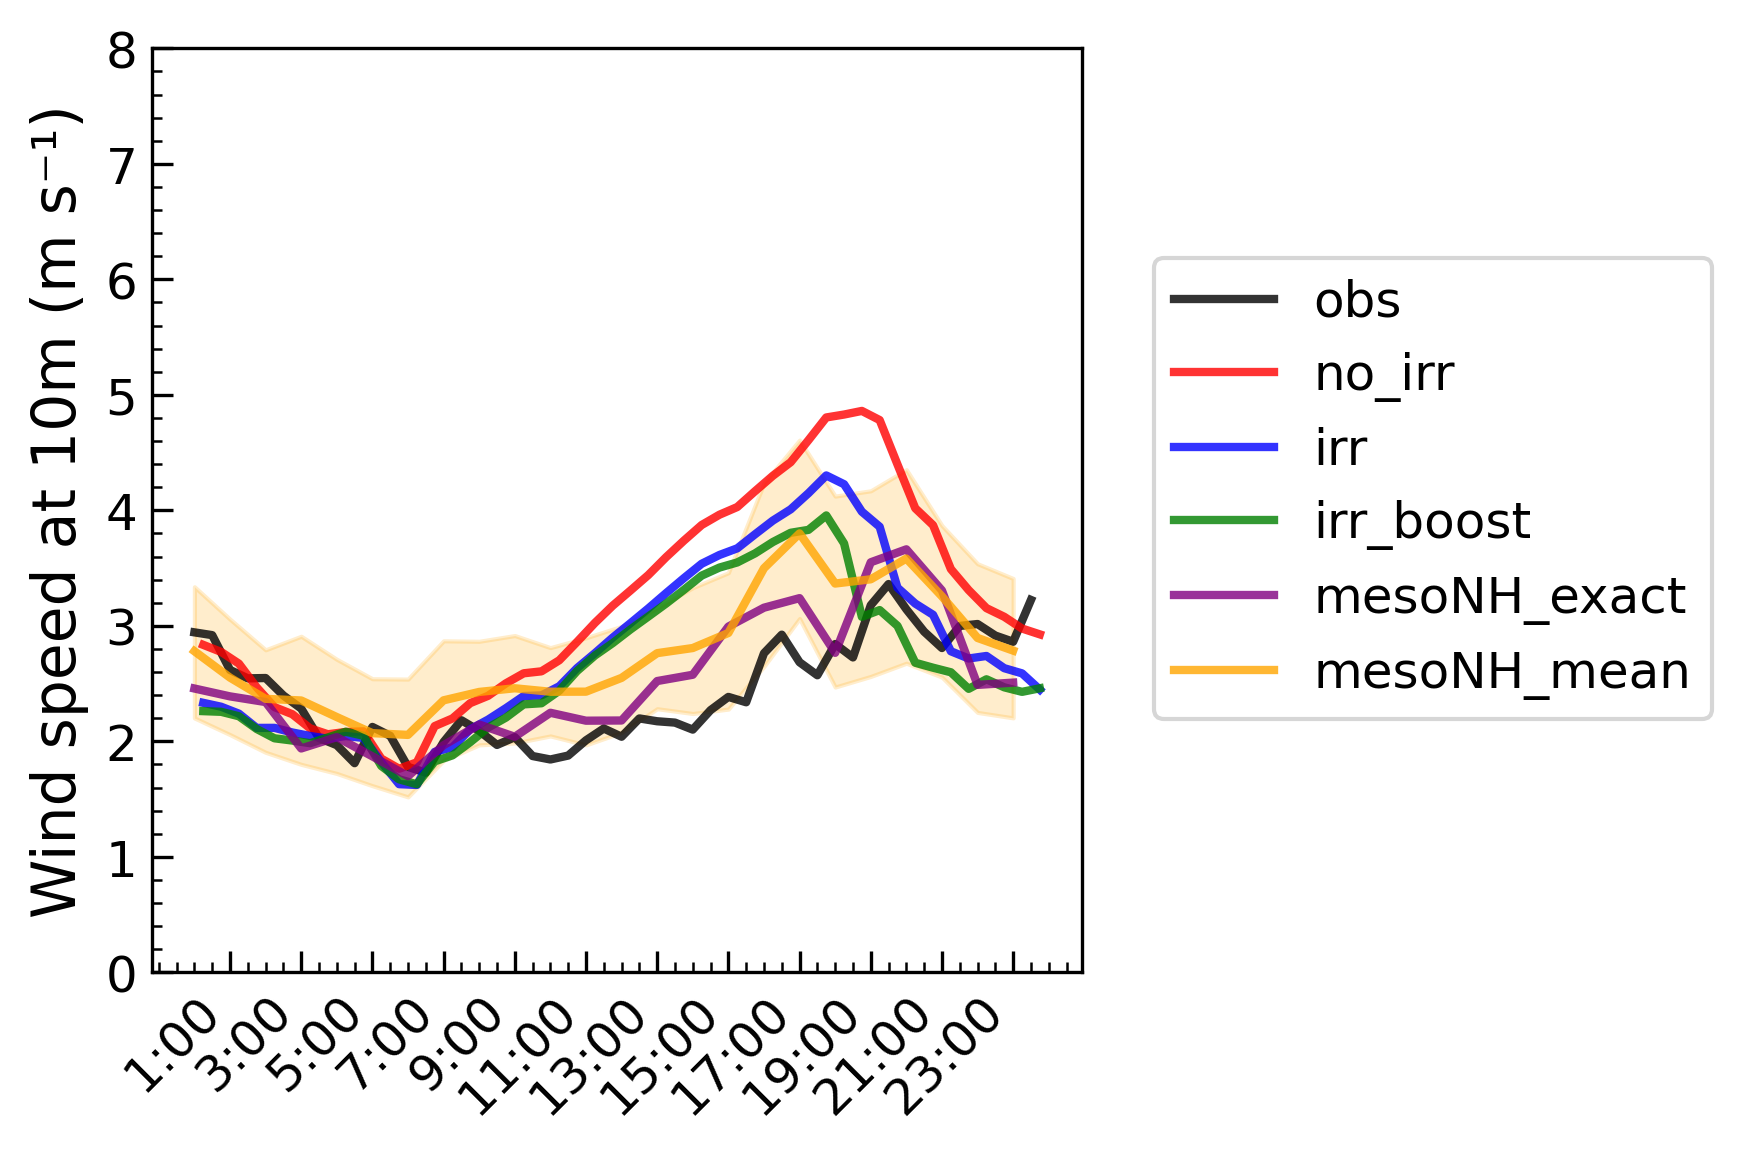
\includegraphics[width=\textwidth]{images/chap5/SOP_TS_DC/diurnal_cycle_cendrosa_wind_speed_10m.png}
        \end{subfigure} \\
        
        \begin{subfigure}[t]{0.5\textwidth}
            \caption{}
            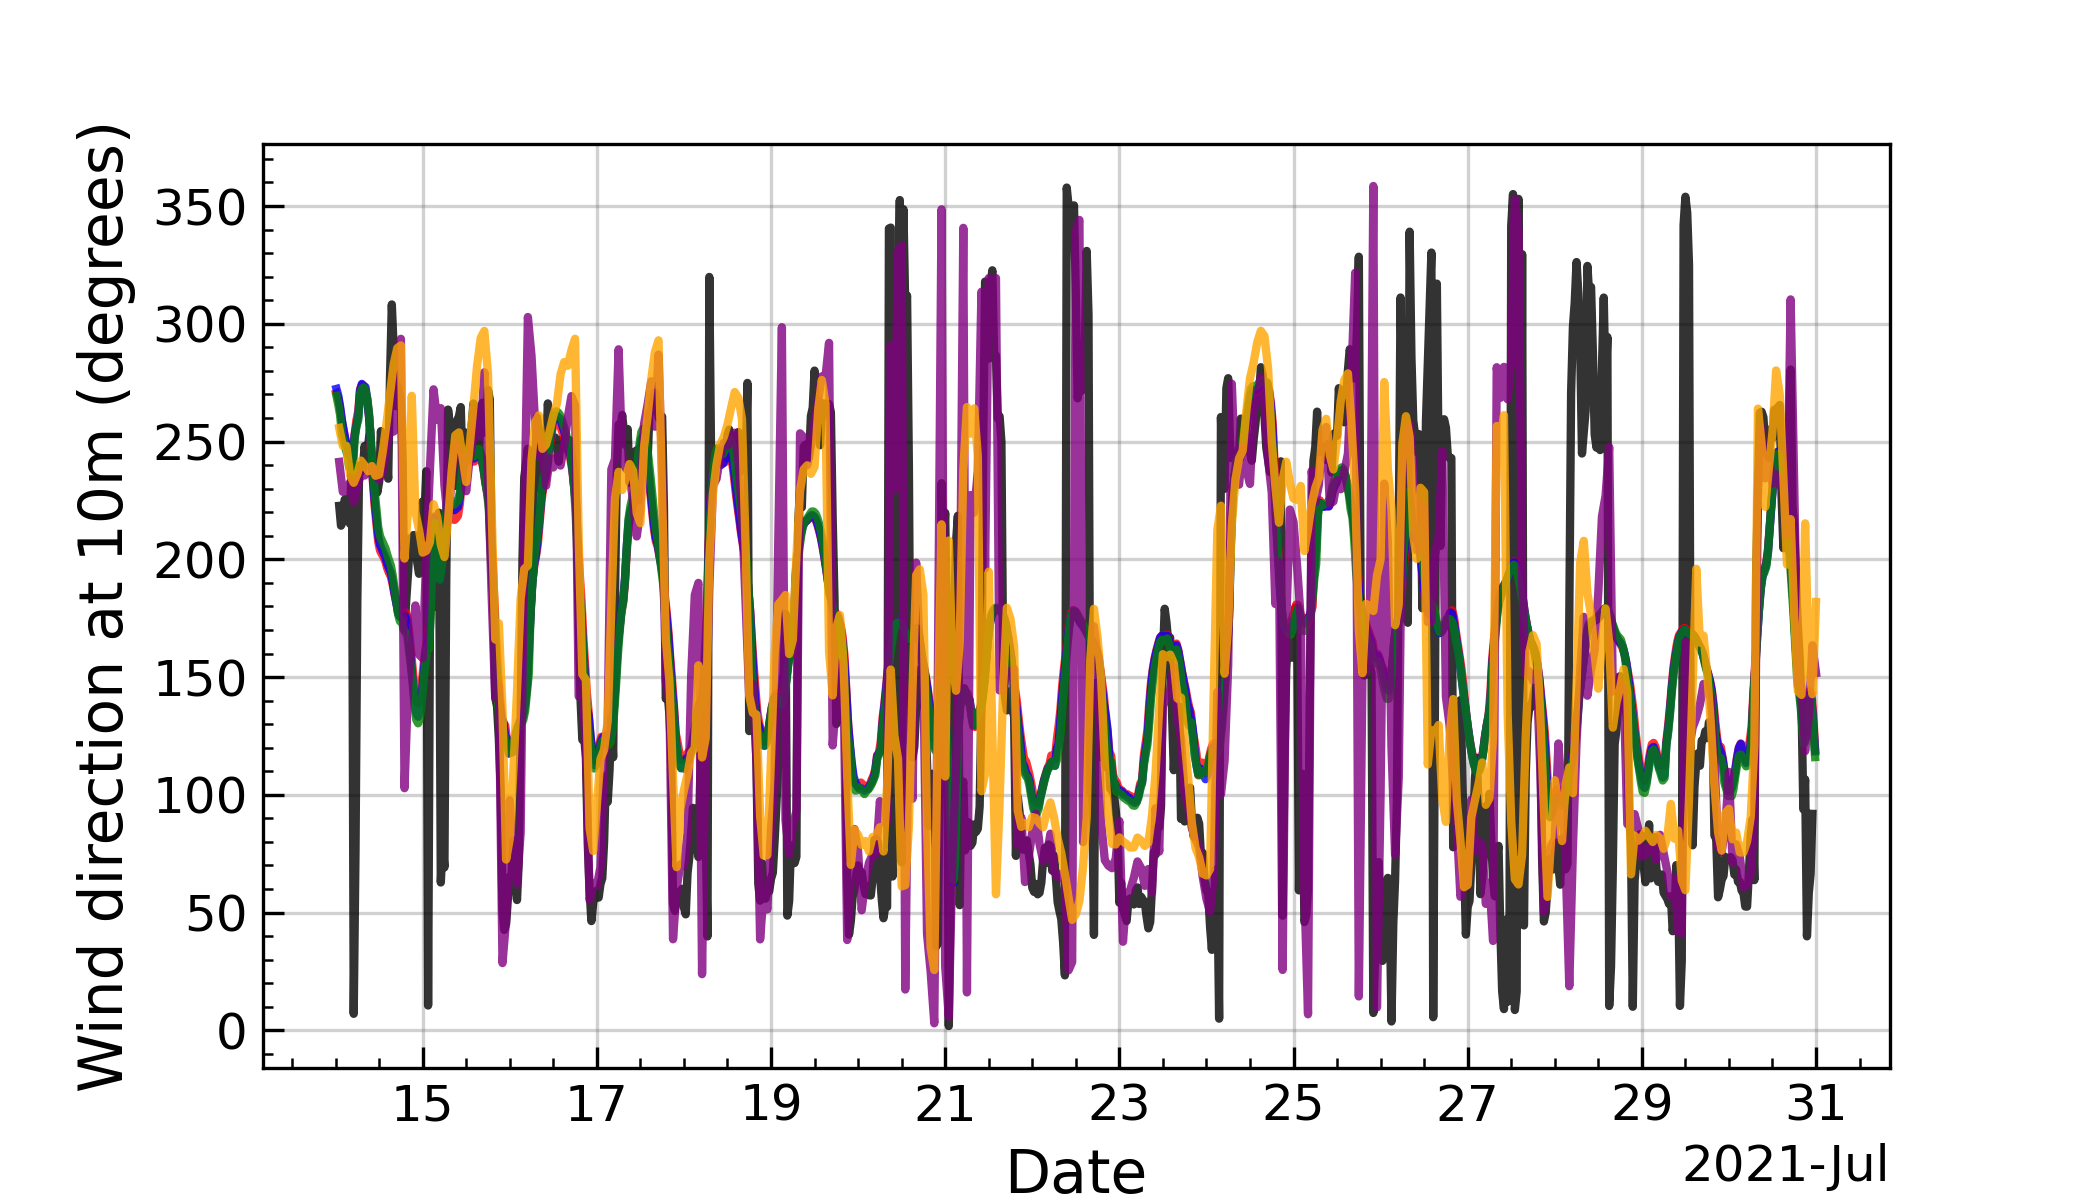
\includegraphics[width=\textwidth]{images/chap5/SOP_TS_DC/time_series_cendrosa_wind_direction_10m.png}
        \end{subfigure} &
        \begin{subfigure}[t]{0.5\textwidth}
            \caption{}
            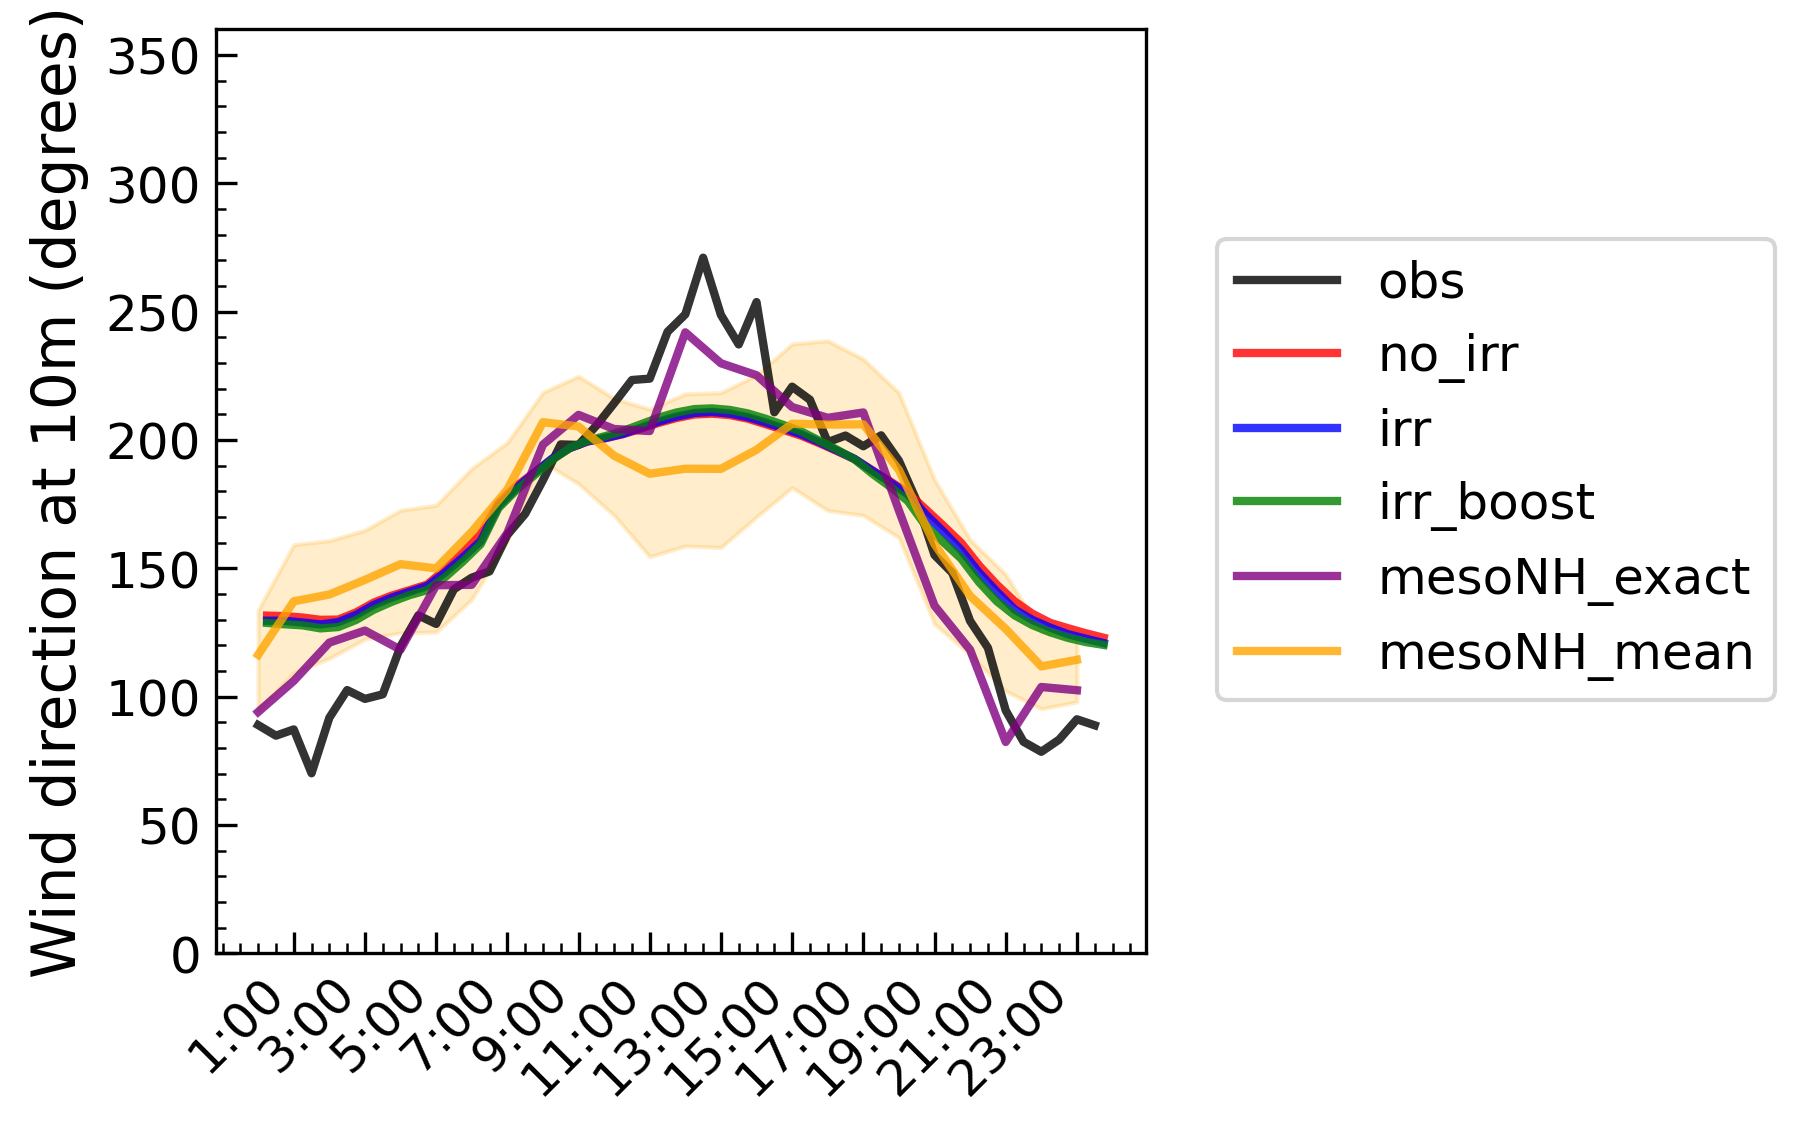
\includegraphics[width=\textwidth]{images/chap5/SOP_TS_DC/diurnal_cycle_cendrosa_wind_direction_10m.png}
        \end{subfigure} \\

        \begin{subfigure}[t]{0.5\textwidth}
            \caption{}
            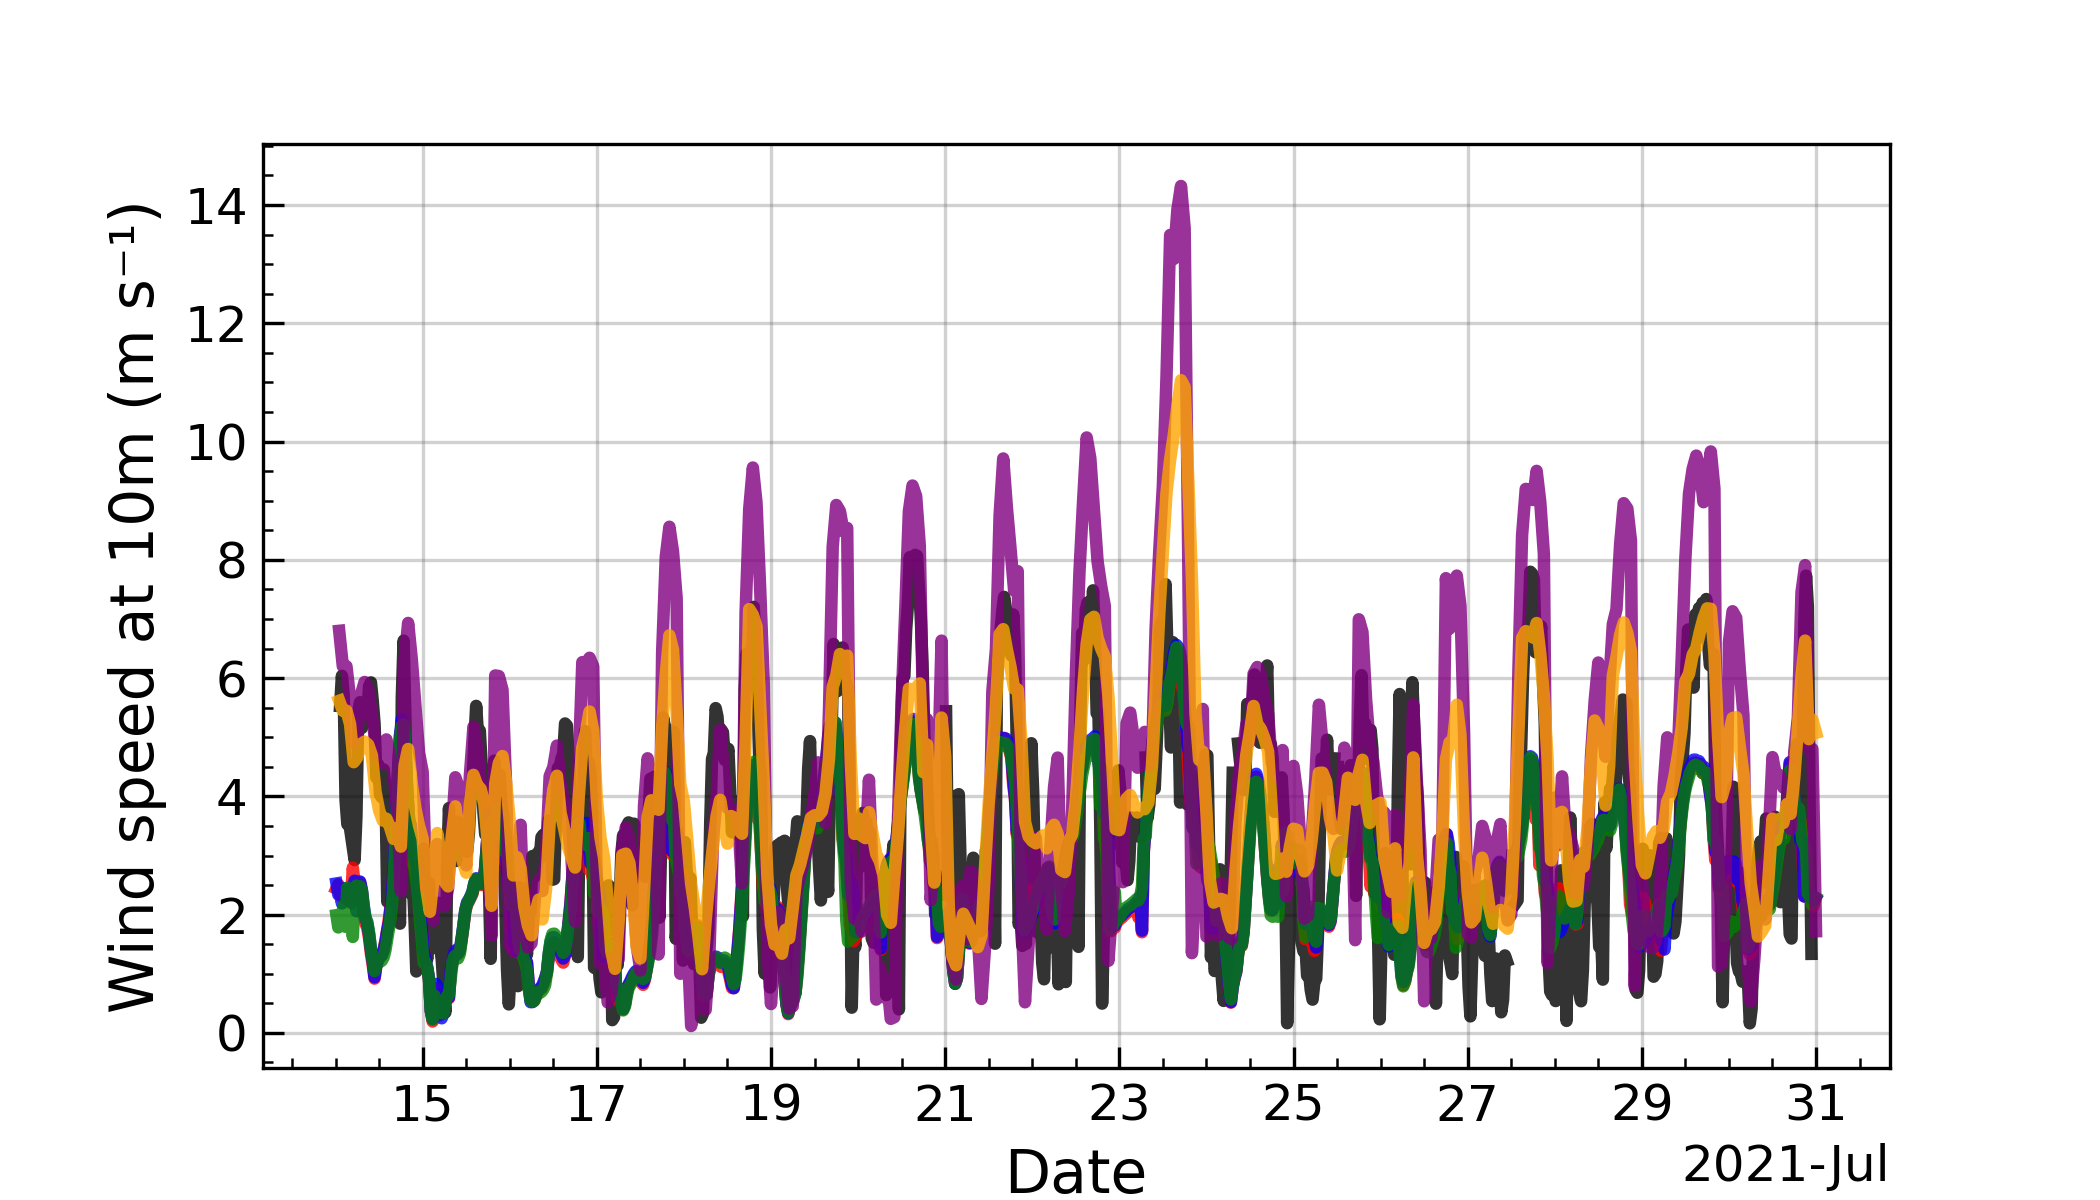
\includegraphics[width=\textwidth]{images/chap5/SOP_TS_DC/time_series_elsplans_wind_speed_10m.png}
        \end{subfigure} &
        \begin{subfigure}[t]{0.5\textwidth}
            \caption{}
            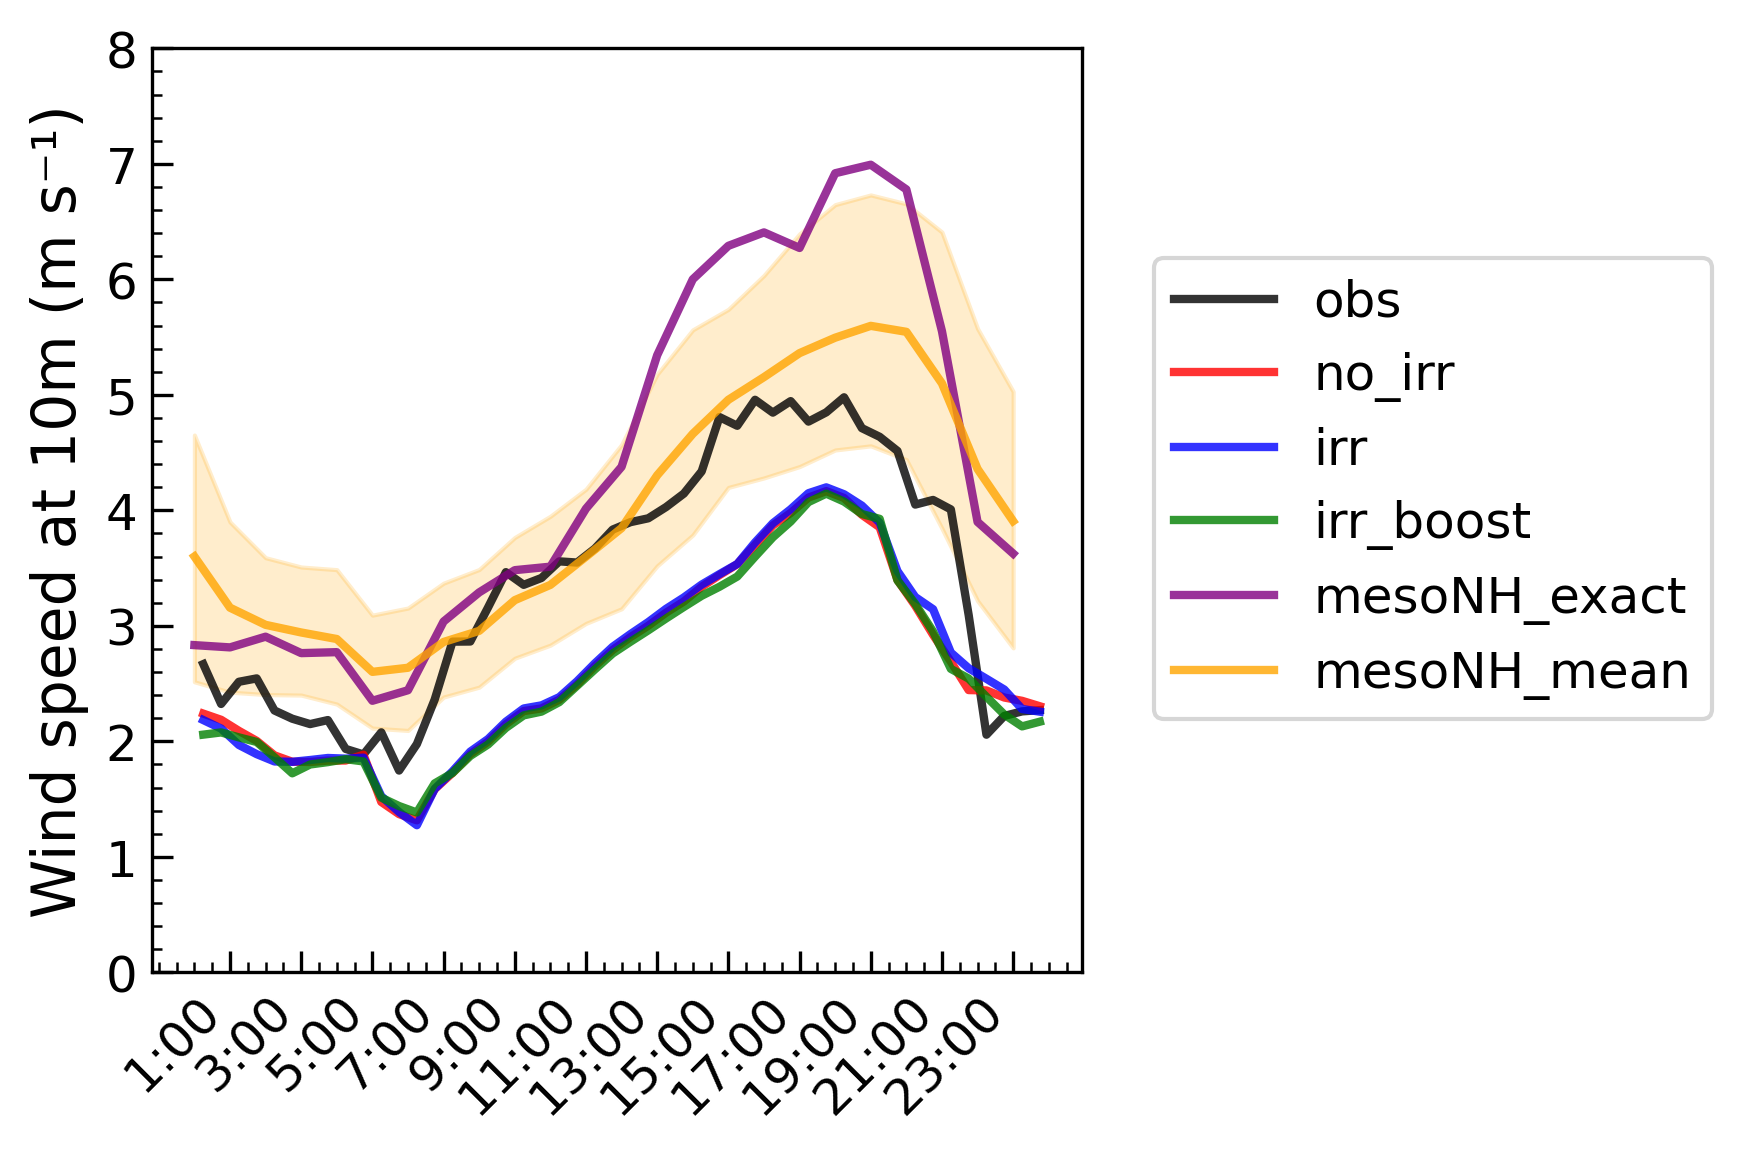
\includegraphics[width=\textwidth]{images/chap5/SOP_TS_DC/diurnal_cycle_elsplans_wind_speed_10m.png}
        \end{subfigure} \\
        
        \begin{subfigure}[t]{0.5\textwidth}
            \caption{}
            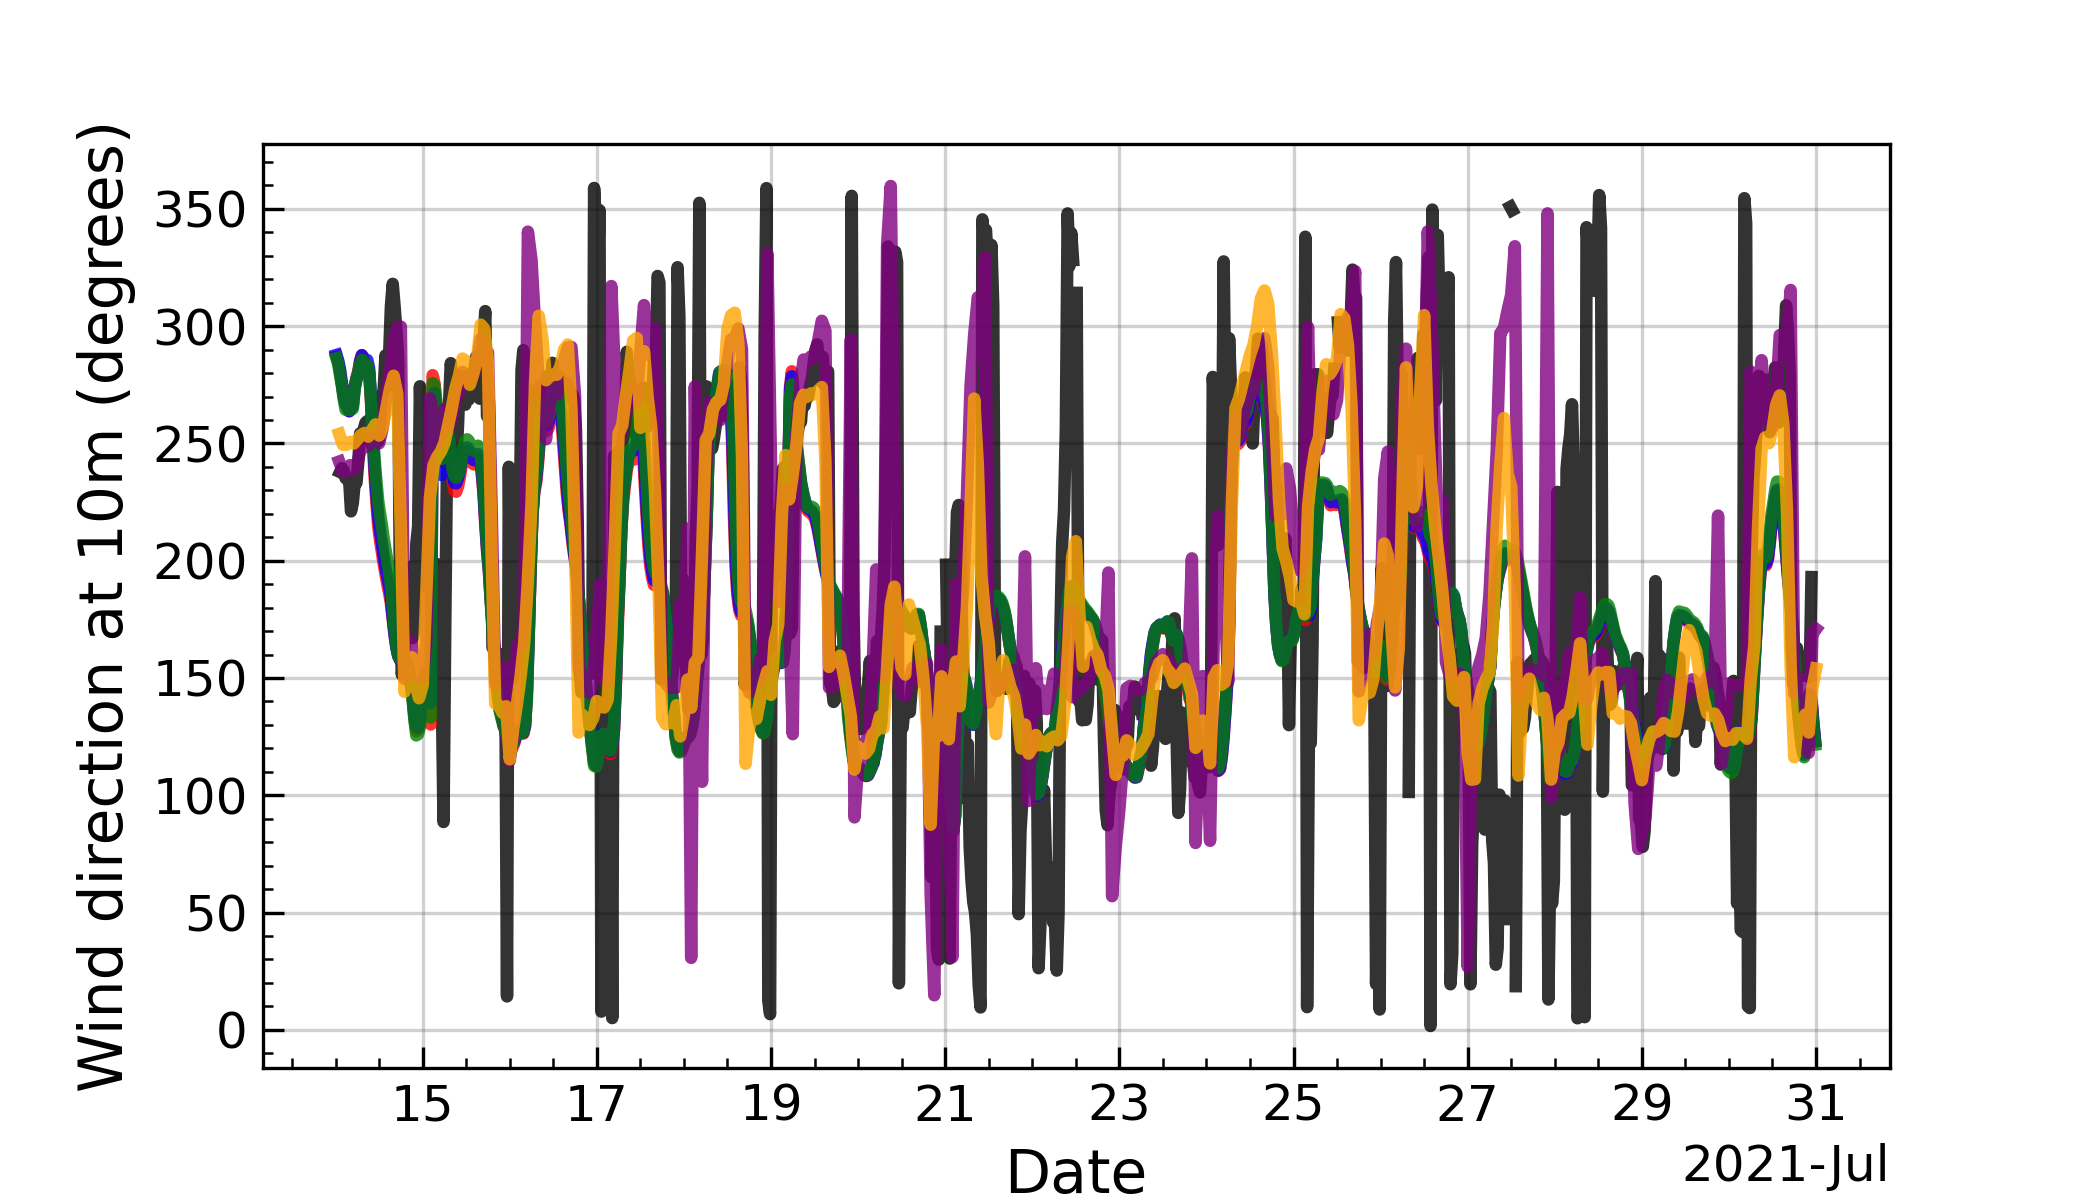
\includegraphics[width=\textwidth]{images/chap5/SOP_TS_DC/time_series_elsplans_wind_direction_10m.png}
        \end{subfigure} &
        \begin{subfigure}[t]{0.5\textwidth}
            \caption{}
            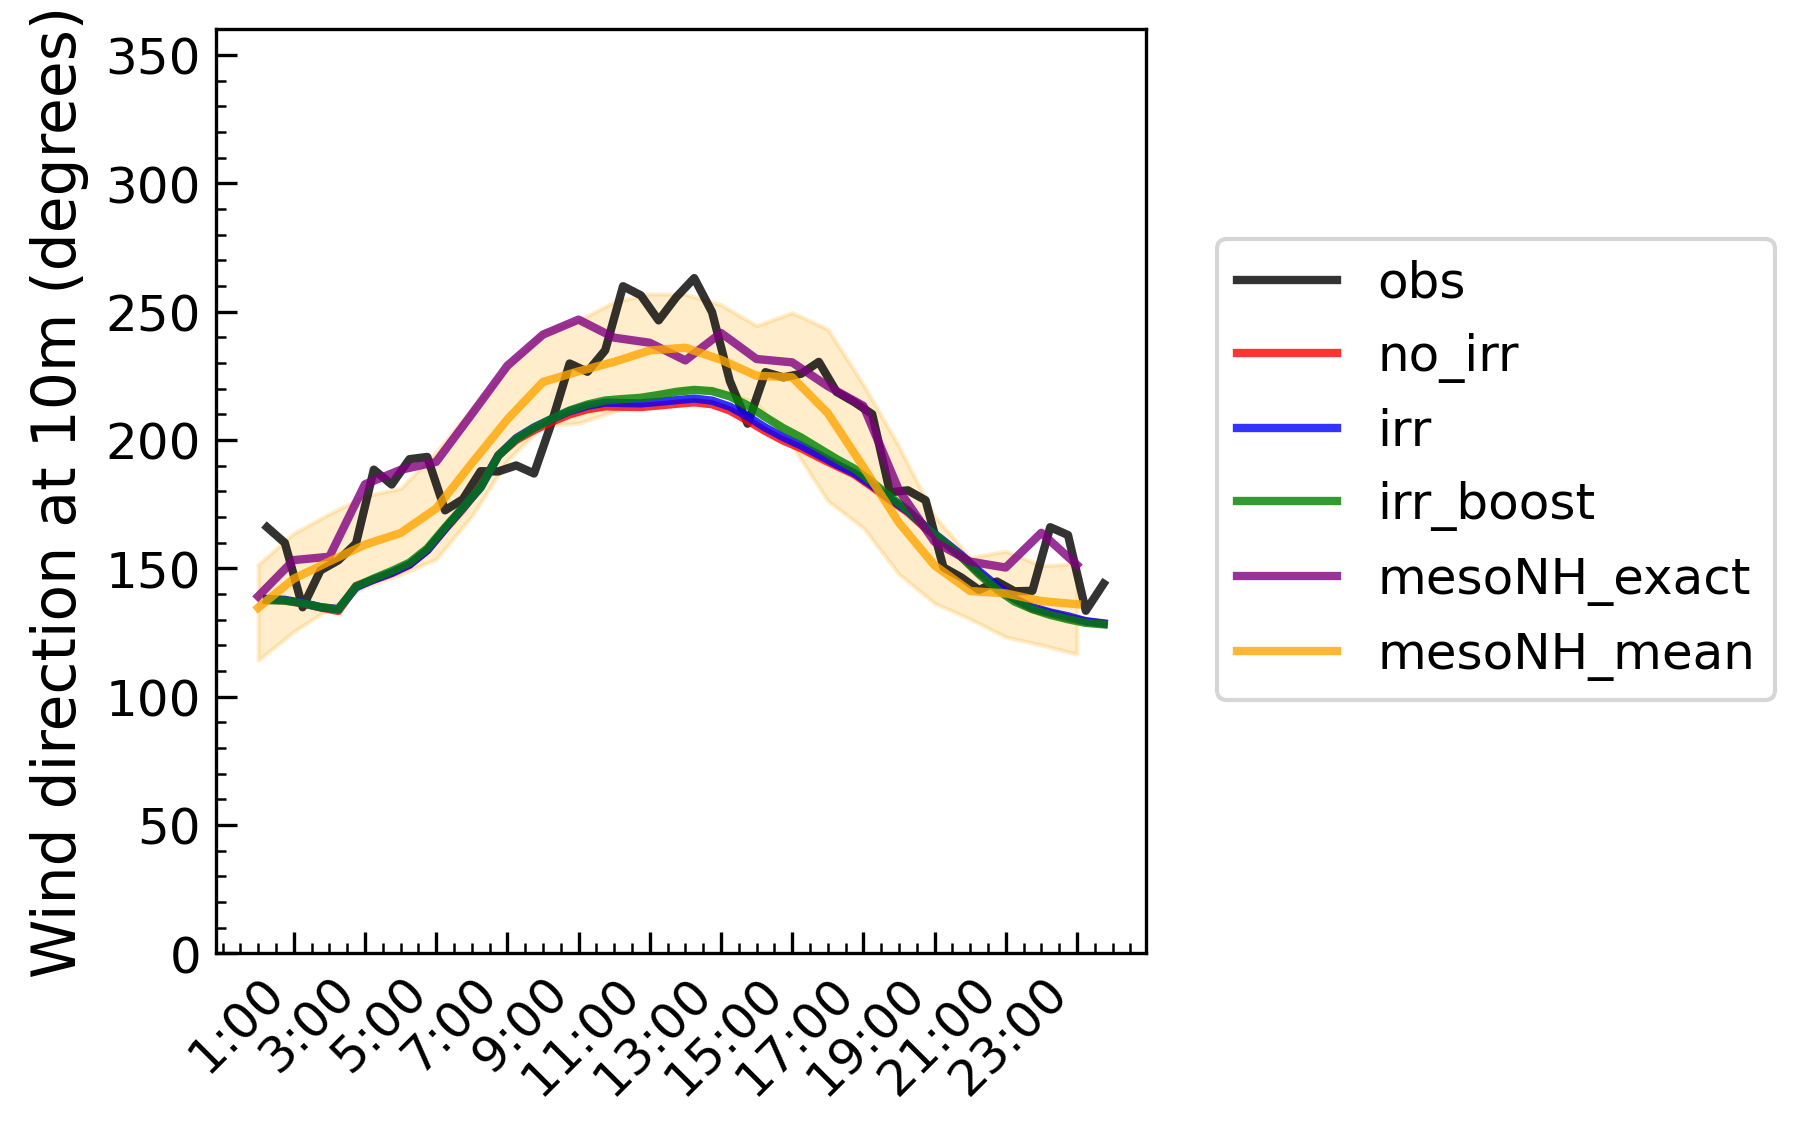
\includegraphics[width=\textwidth]{images/chap5/SOP_TS_DC/diurnal_cycle_elsplans_wind_direction_10m.png}
        \end{subfigure} \\
    \end{tabular}
    \caption{Time series and mean diurnal cycle of wind speed and direction on both sites, July 14-30 2021.}
    \label{fig:bothsites_wind}
\end{figure}

\clearpage

\section{Vertical structure of the atmosphere}
\label{sec:iop}

Out of the seven IOP days over which radiosoundings were conducted on both sites, two were selected (July 15th and 20th) to investigate the atmospheric behaviour of the ICOLMDZOR LAM and the impact of irrigation on the vertical structure of the ABL.

\subsection{Surface conditions on selected IOP days}
%todo:reorganize, describe obs for all vars and then comment on model performance ?
%mesoexact is very very good on most vars, making it an interesting reference

July 15th was selected as a representative IOP day for the beginning of the SOP, showing similarities with observed profiles on the 16th and 17th. As the SOP progressed, 2-meter temperature increased and the wind regime became much more changeable, with more influence from the sea breeze circulation.
The three following IOP days (20th, 21st, 22nd) therefore presented different conditions, and this is why July 20th was also selected to analyse the impacts of irrigation on the ABL under different conditions.
The time series at La Cendrosa over both days show that July 20th was a warmer day than July 15th (Fig. \ref{fig:iop_days_TS_energy}a,b) and that the lower atmospher was moister (Fig. \ref{fig:iop_days_TS_energy}c,d).
%LMDZ biases in t2m, q2m
At the surface, ICOLMDZOR presents a warm bias on July 15th but almost not temperature bias in the \irrboost simulation on July 20th. As previously noticed in general over the SOP, 2-m specific humidity is overestimated by ICOLMDZOR at night, but decreases during the day. In \irrboost, it remains slightly above observed and MesoNH values during the day on July 15th, but on July 20th it is underestimated.
%link to flat
This may partly be explained by the simulated latent heat flux.%todo:meh
In the first part of the SOP, the alfalfa crops at La Cendrosa were still freshly cut and had not recovered their original size, LAI and transpiration levels. 
Since the models do not account for this information, the latent heat flux is overestimated by MesoNH (both \mesoexact and \mesomean are above the observations) and ICOLMDZOR (in the \irrboost simulation), whereas the sensible heat flux is underestimated (Fig. \ref{fig:iop_days_TS_energy}e, g). 
On July 20th, observed latent heat flux is higher and sensible heat flux lower, even presenting negative values in the afternoon.
It is difficult to disentangle the increase due to the vegetation growth from the increased evaporative demand due to the warming, but in \mesoexact, the increase is rather small.%blah
For both turbulent fluxes, as noticed in Section \ref{sec:sop}, the \irrboost simulation matches really well the \mesomean aggregated value throughout the day. It is also the case for 2-meter temperature but not really for specific humidity and 10m winds, which might result from limitations of the dynamics rather than the LMDZ physics.

% However, MesoNH does not overestimate 2-meter specific humidity, and  


%Fig : energy fluxes Cendrosa
\begin{figure}[hbtp]
    \centering
    \begin{tabular}{cc}
        %rad fluxes
        \begin{subfigure}[t]{0.5\textwidth}
            \caption{}
            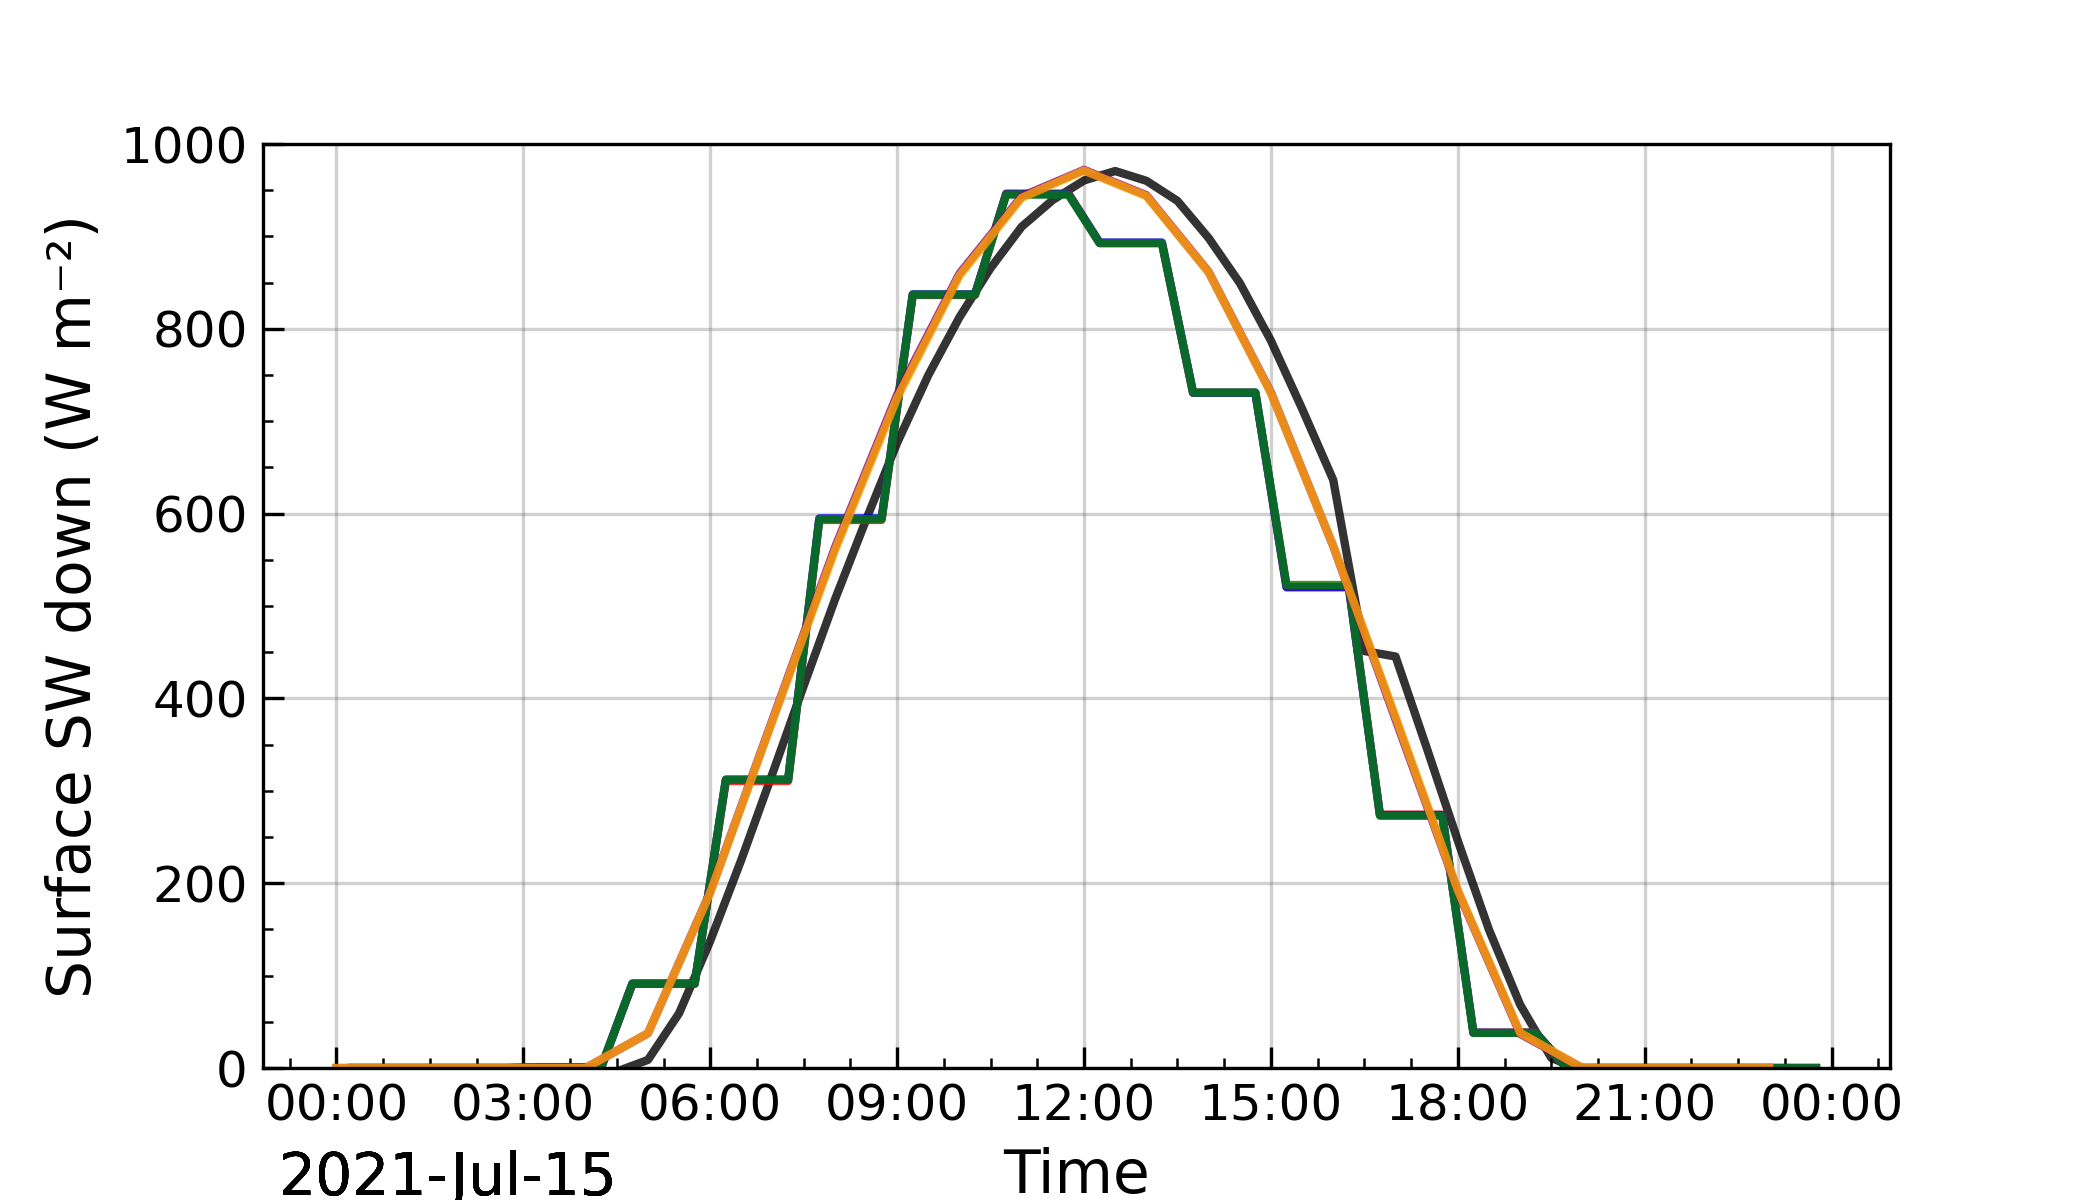
\includegraphics[width=\textwidth]{images/chap5/IOP_TS/TS_2021-07-15_cendrosa_SWdnSFC.png}
        \end{subfigure} &
        \begin{subfigure}[t]{0.5\textwidth}
            \caption{}
            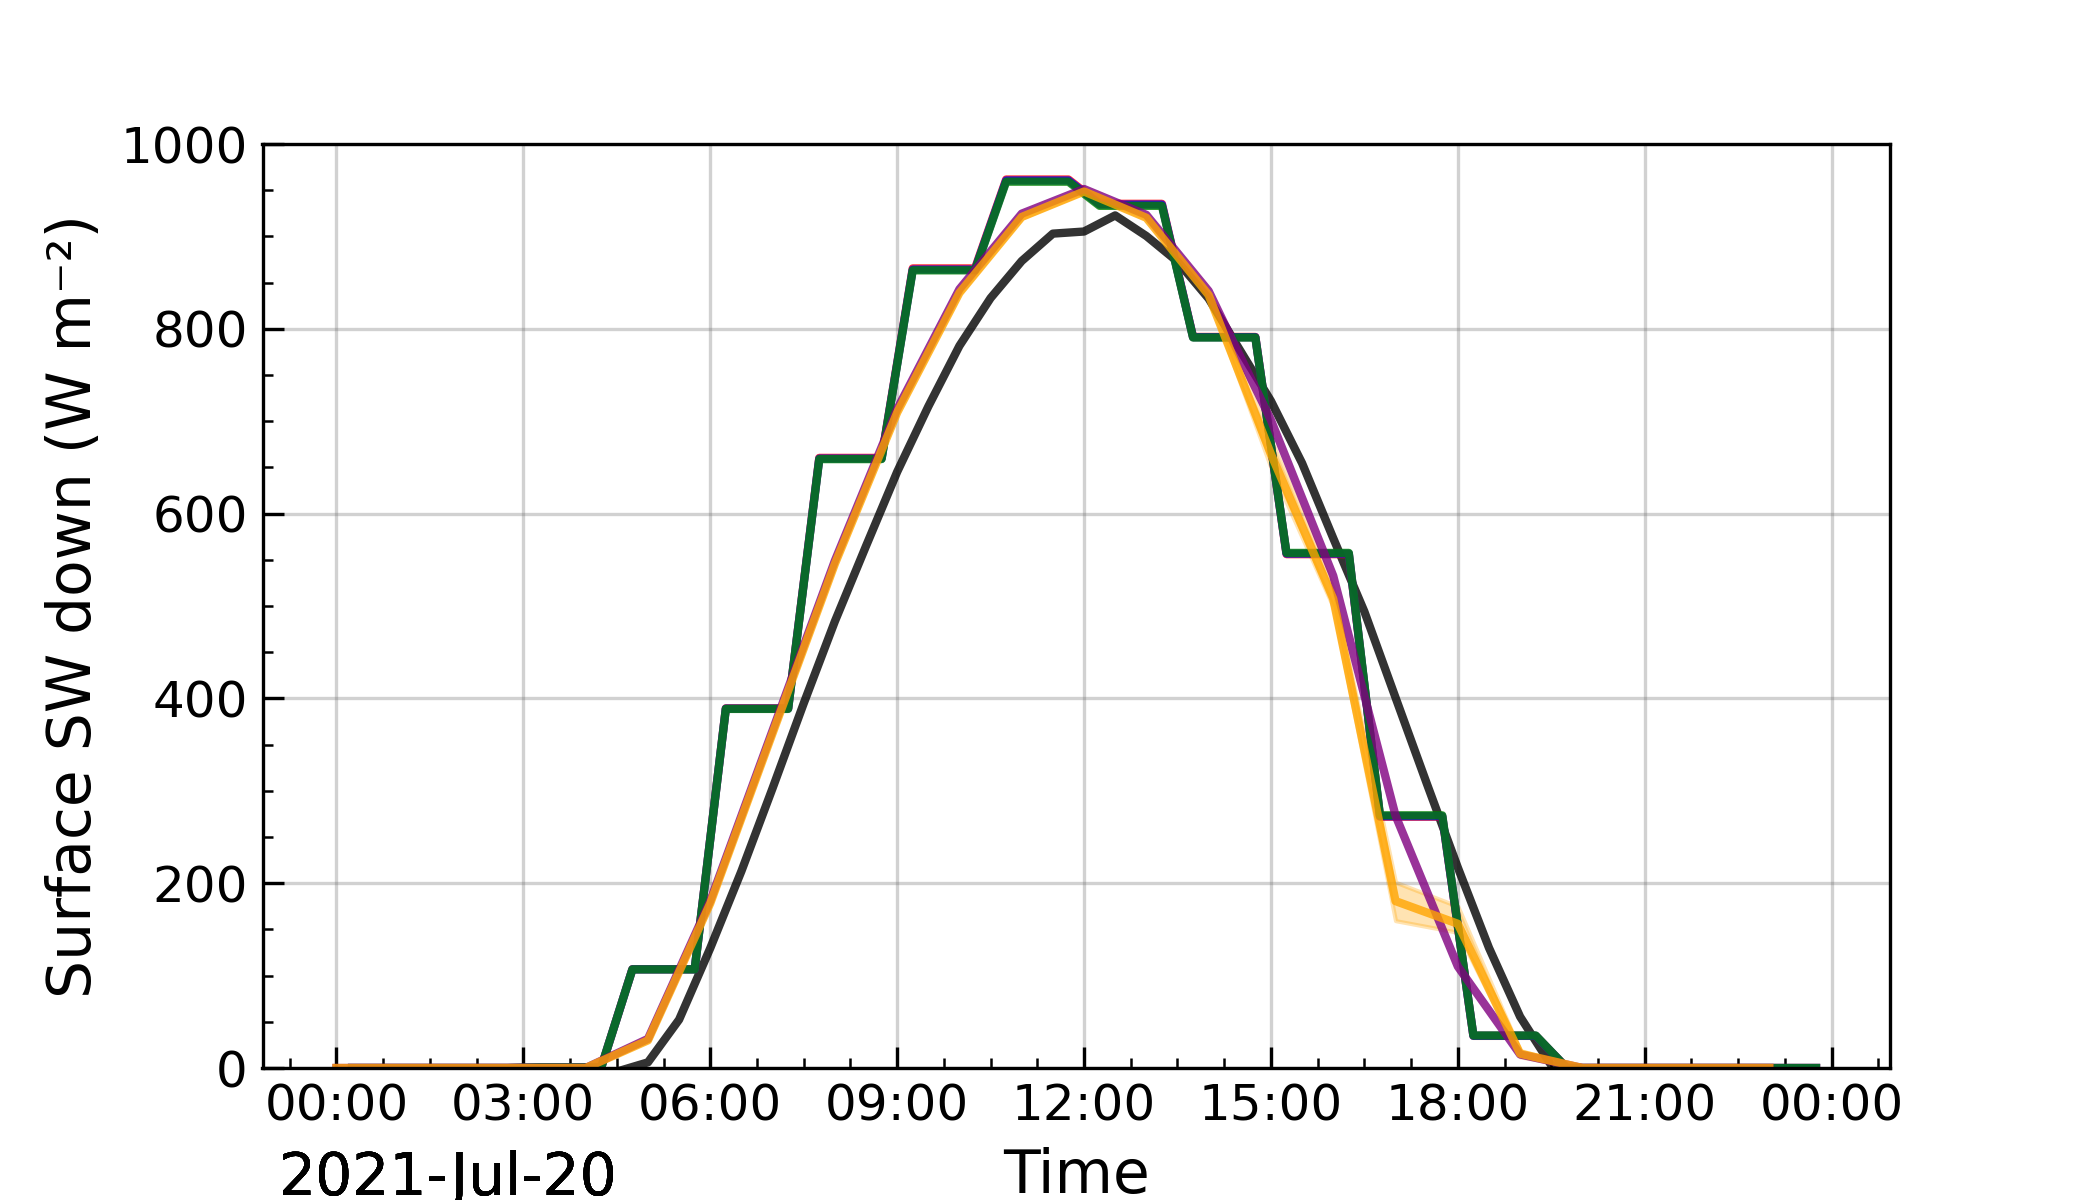
\includegraphics[width=\textwidth]{images/chap5/IOP_TS/TS_2021-07-20_cendrosa_SWdnSFC.png}
        \end{subfigure} \\
        \begin{subfigure}[t]{0.5\textwidth}
            \caption{}
            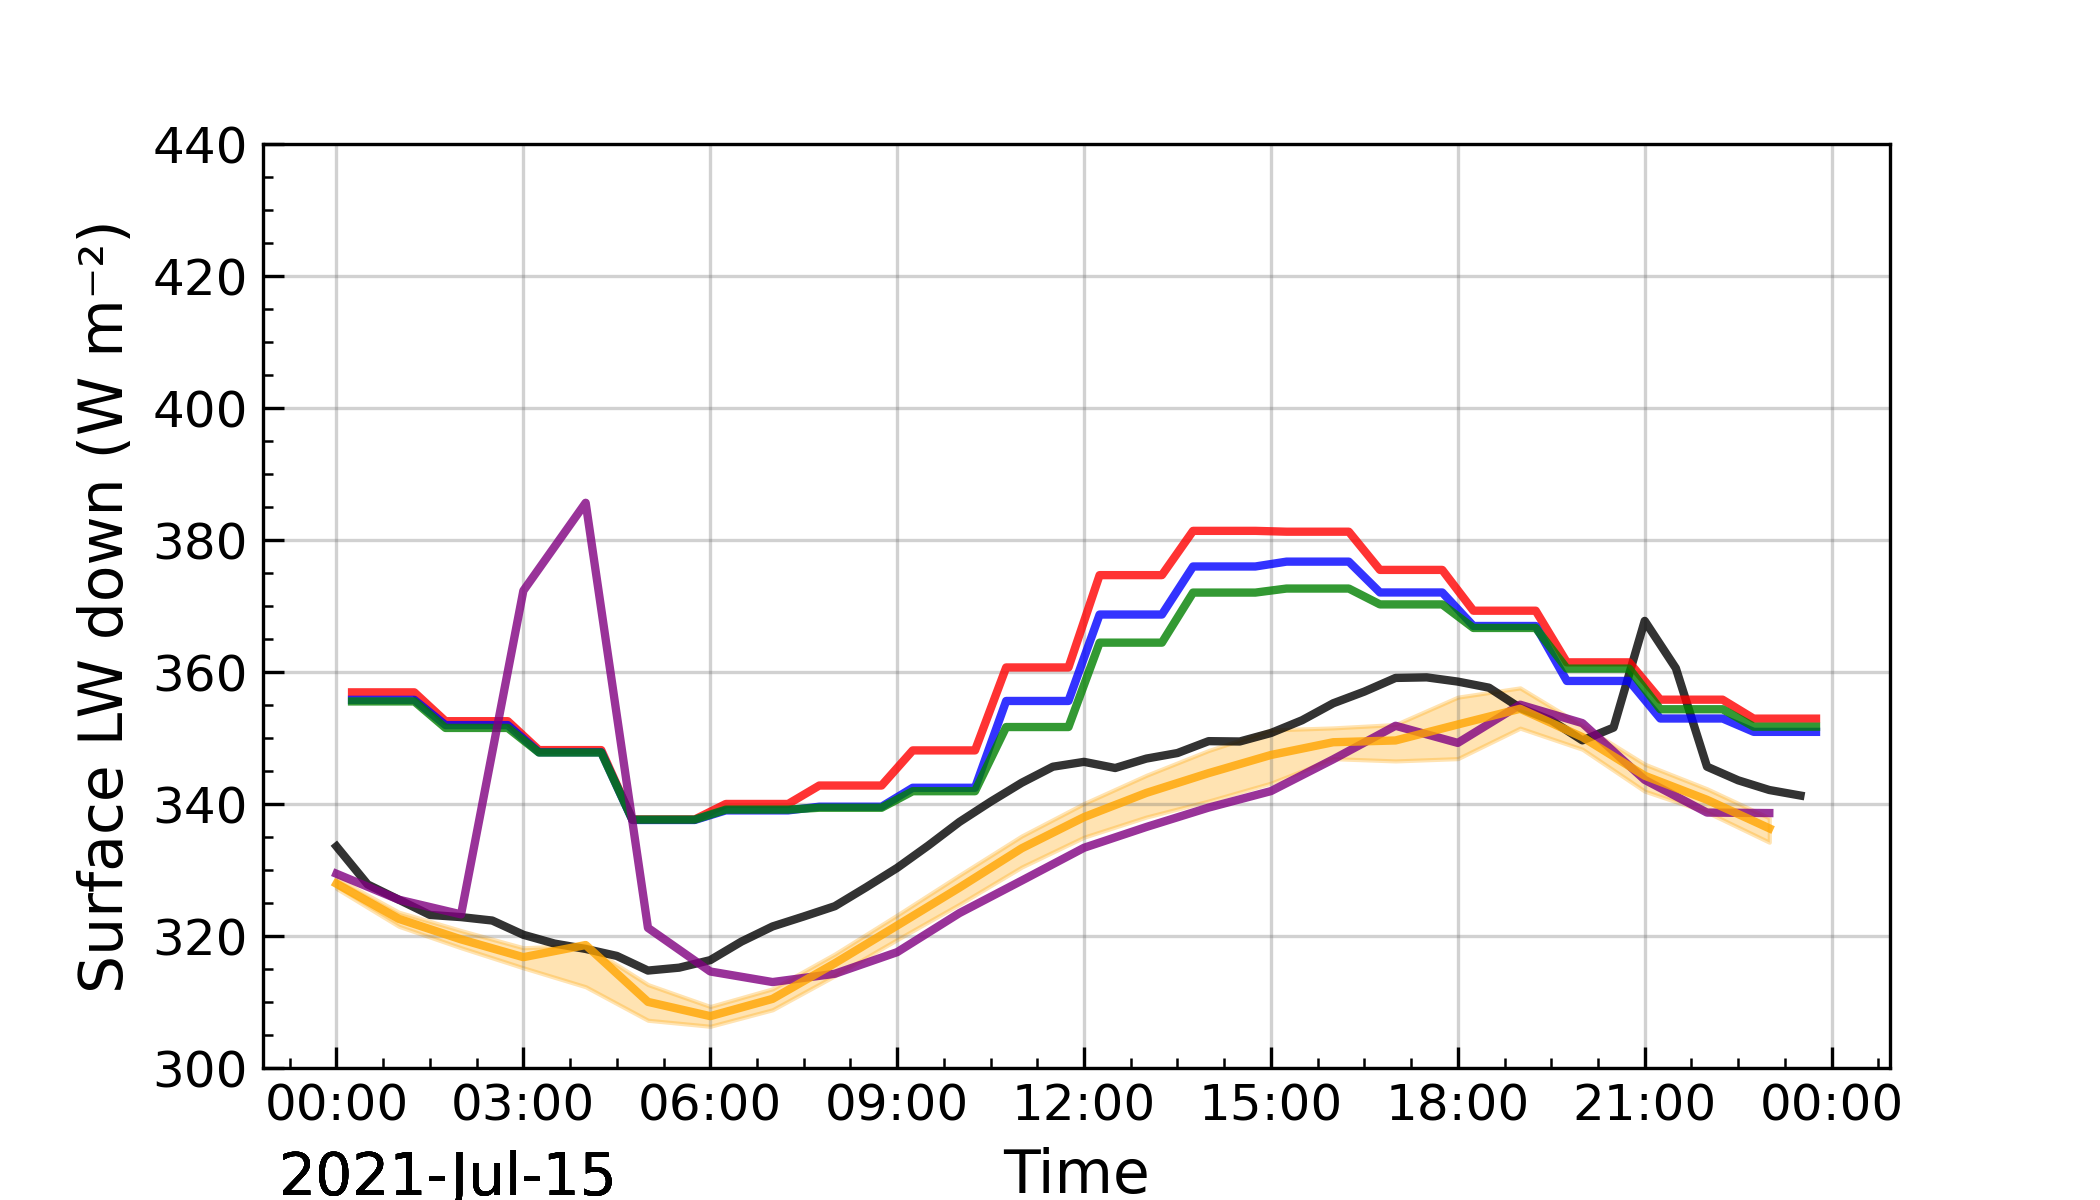
\includegraphics[width=\textwidth]{images/chap5/IOP_TS/TS_2021-07-15_cendrosa_LWdnSFC.png}
        \end{subfigure} &
        \begin{subfigure}[t]{0.5\textwidth}
            \caption{}
            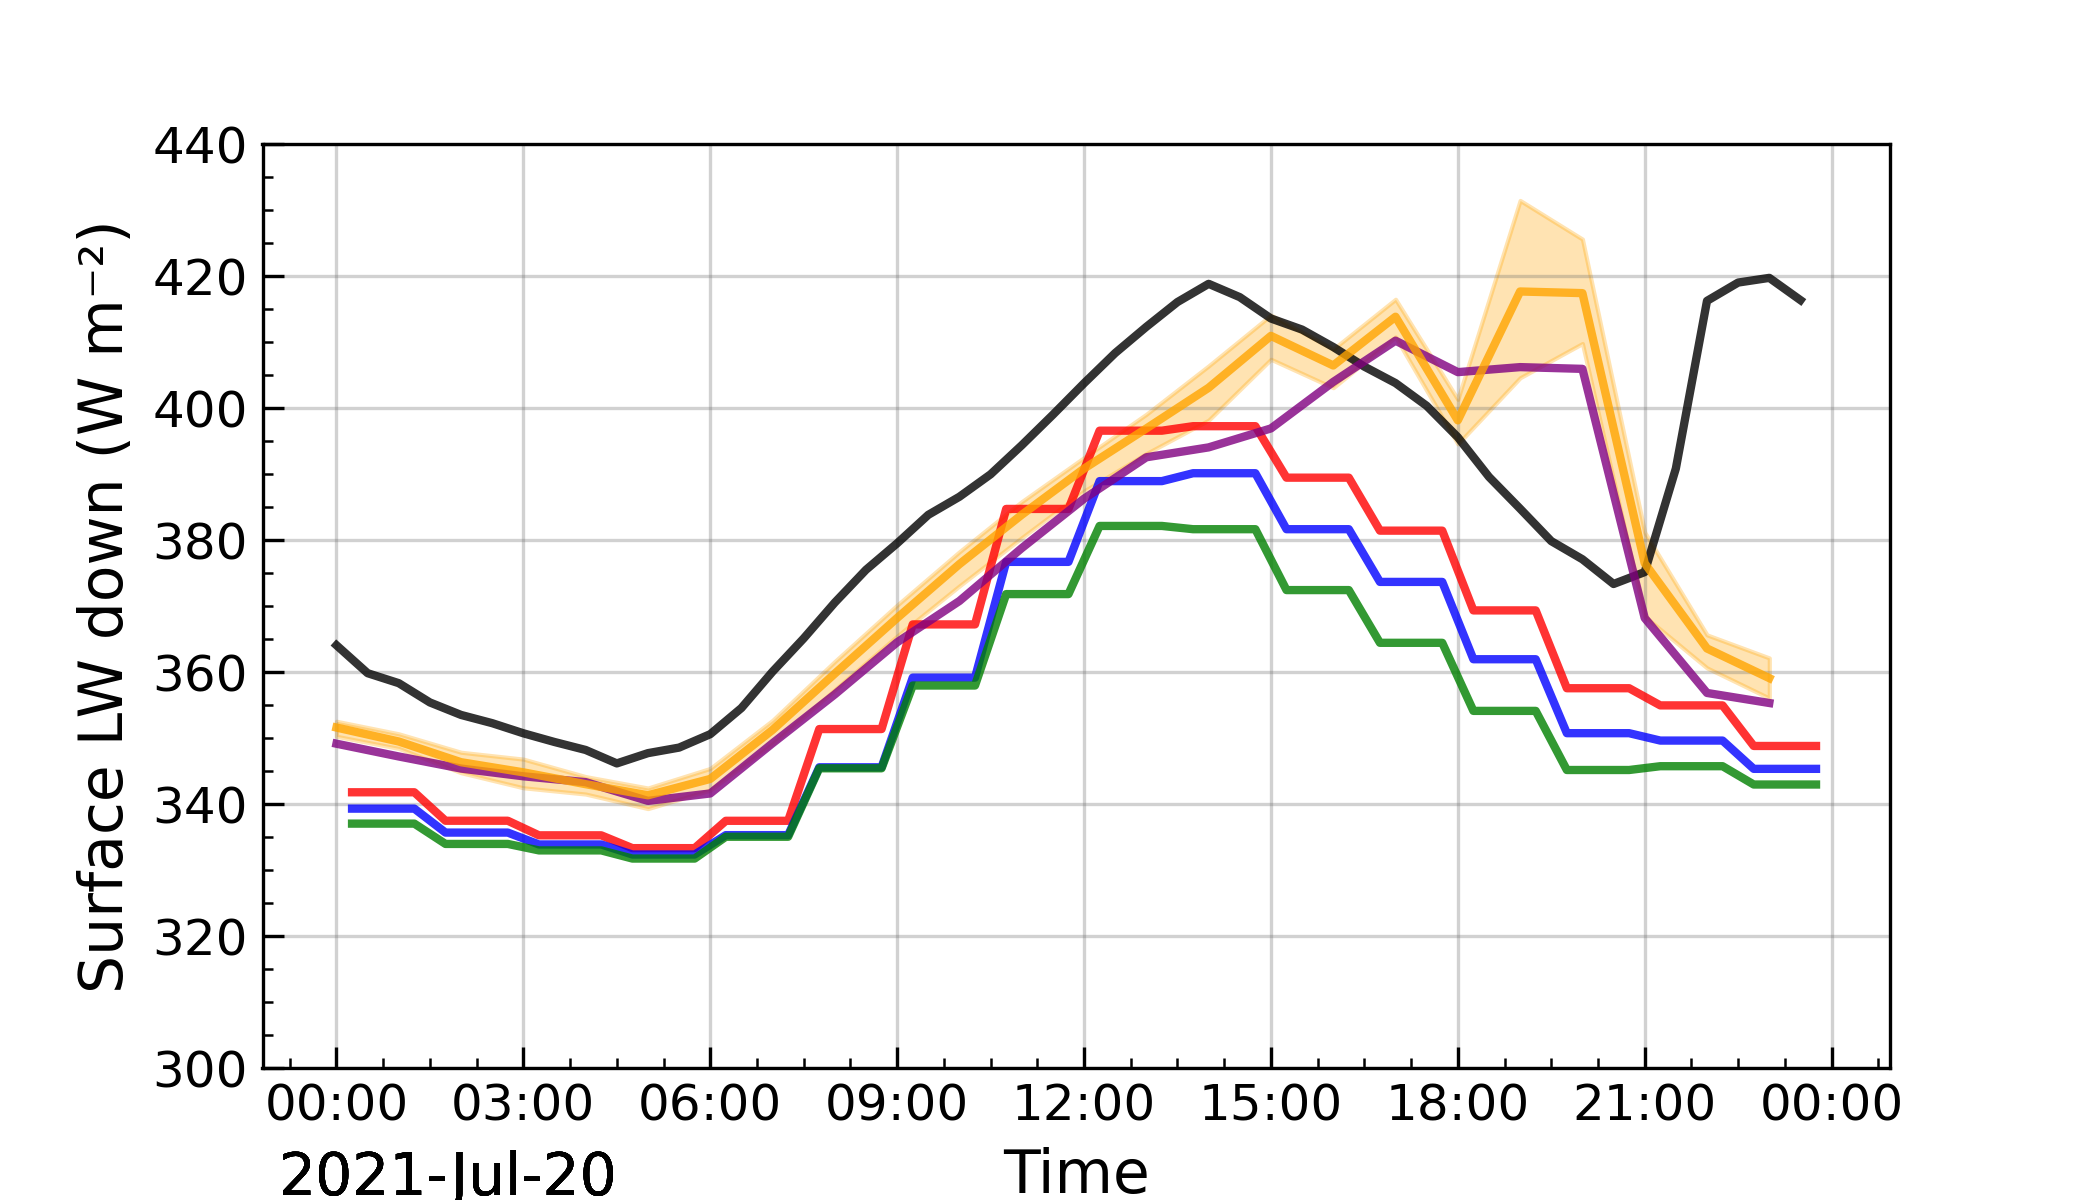
\includegraphics[width=\textwidth]{images/chap5/IOP_TS/TS_2021-07-20_cendrosa_LWdnSFC.png}
        \end{subfigure} \\

        %turb fluxes
        \begin{subfigure}[t]{0.5\textwidth}
            \caption{}
            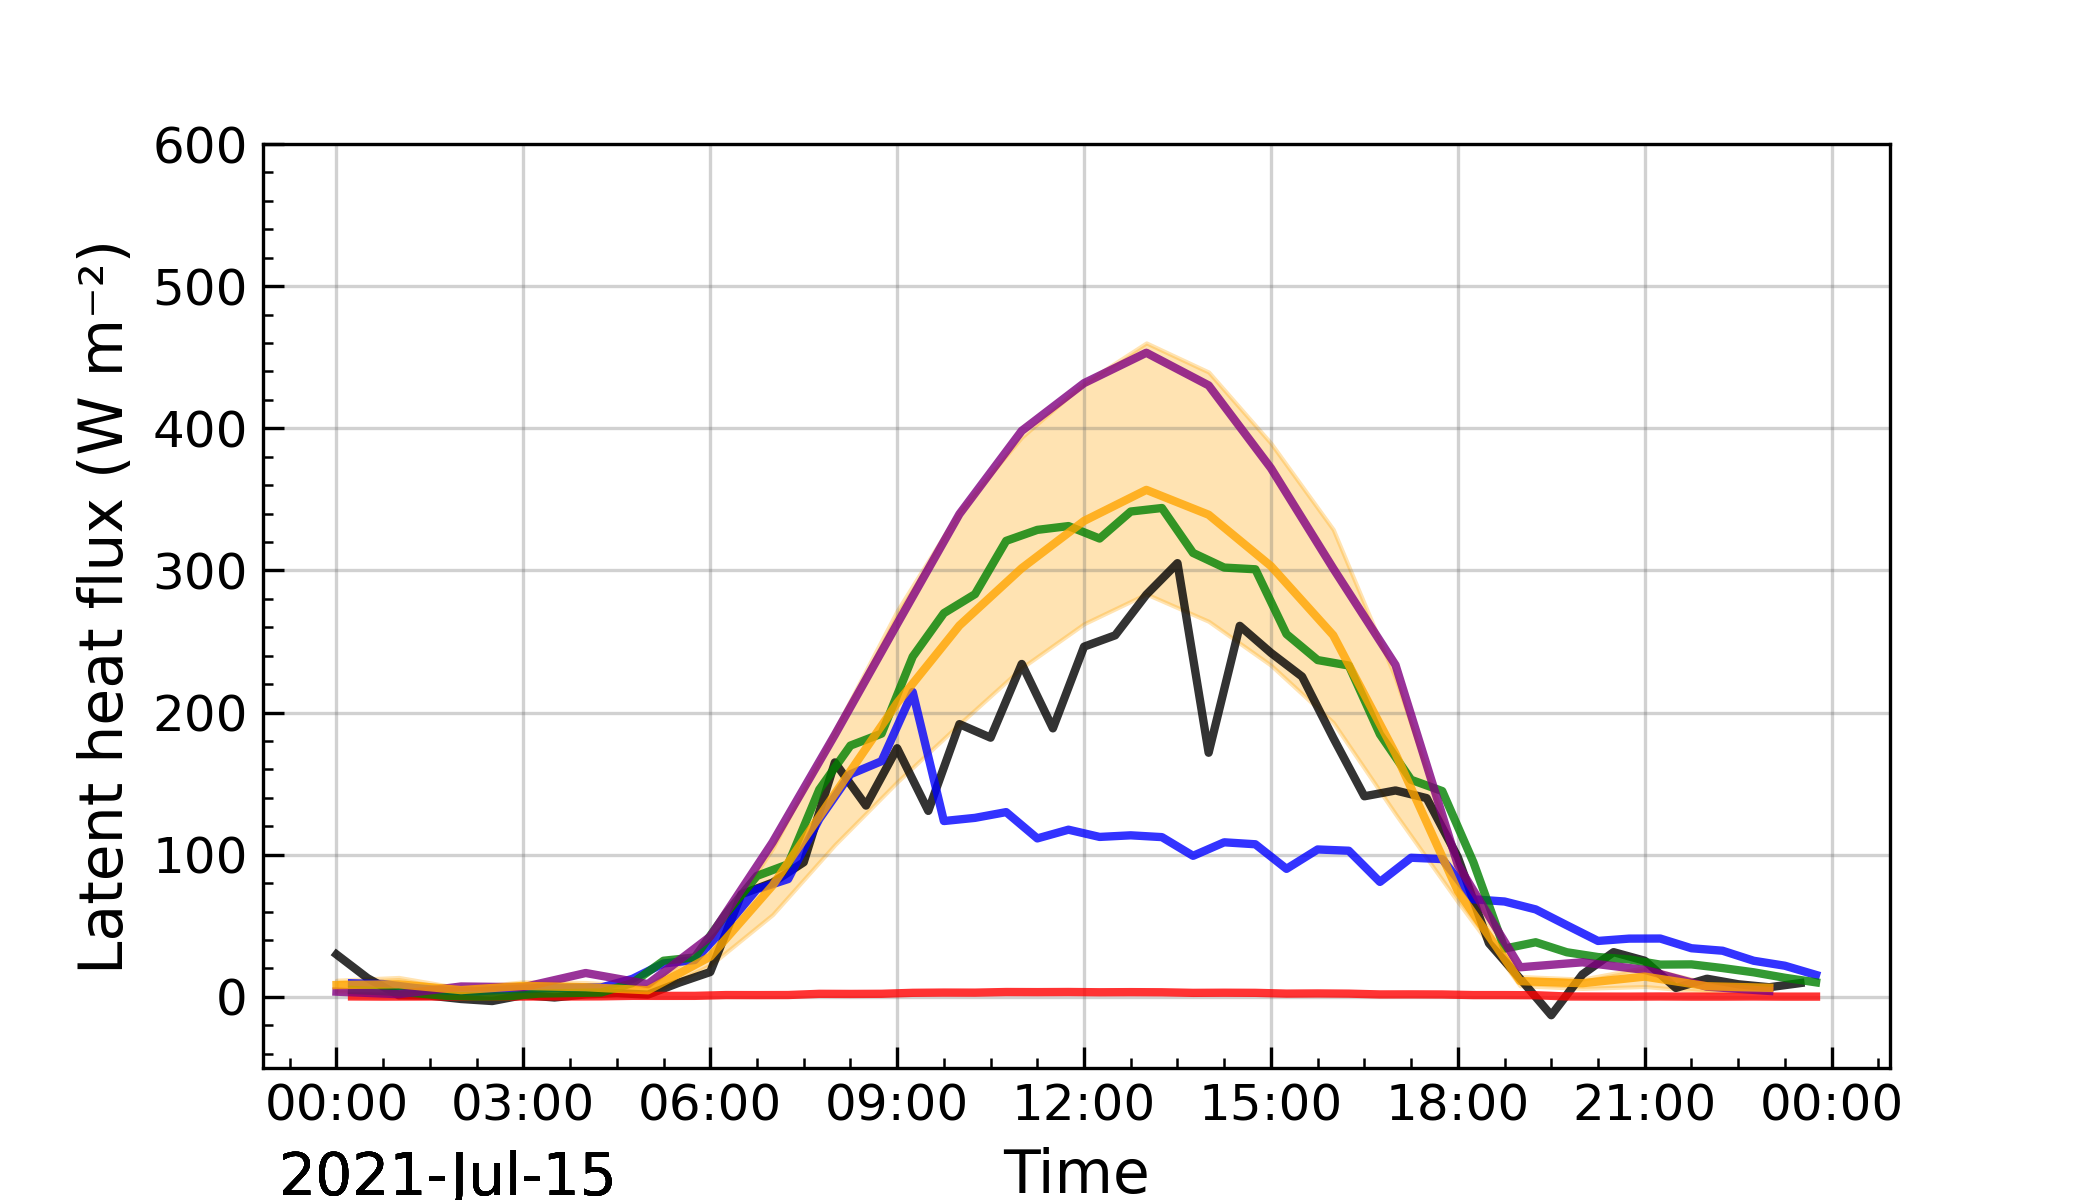
\includegraphics[width=\textwidth]{images/chap5/IOP_TS/TS_2021-07-15_cendrosa_flat.png}
        \end{subfigure} &
        \begin{subfigure}[t]{0.5\textwidth}
            \caption{}
            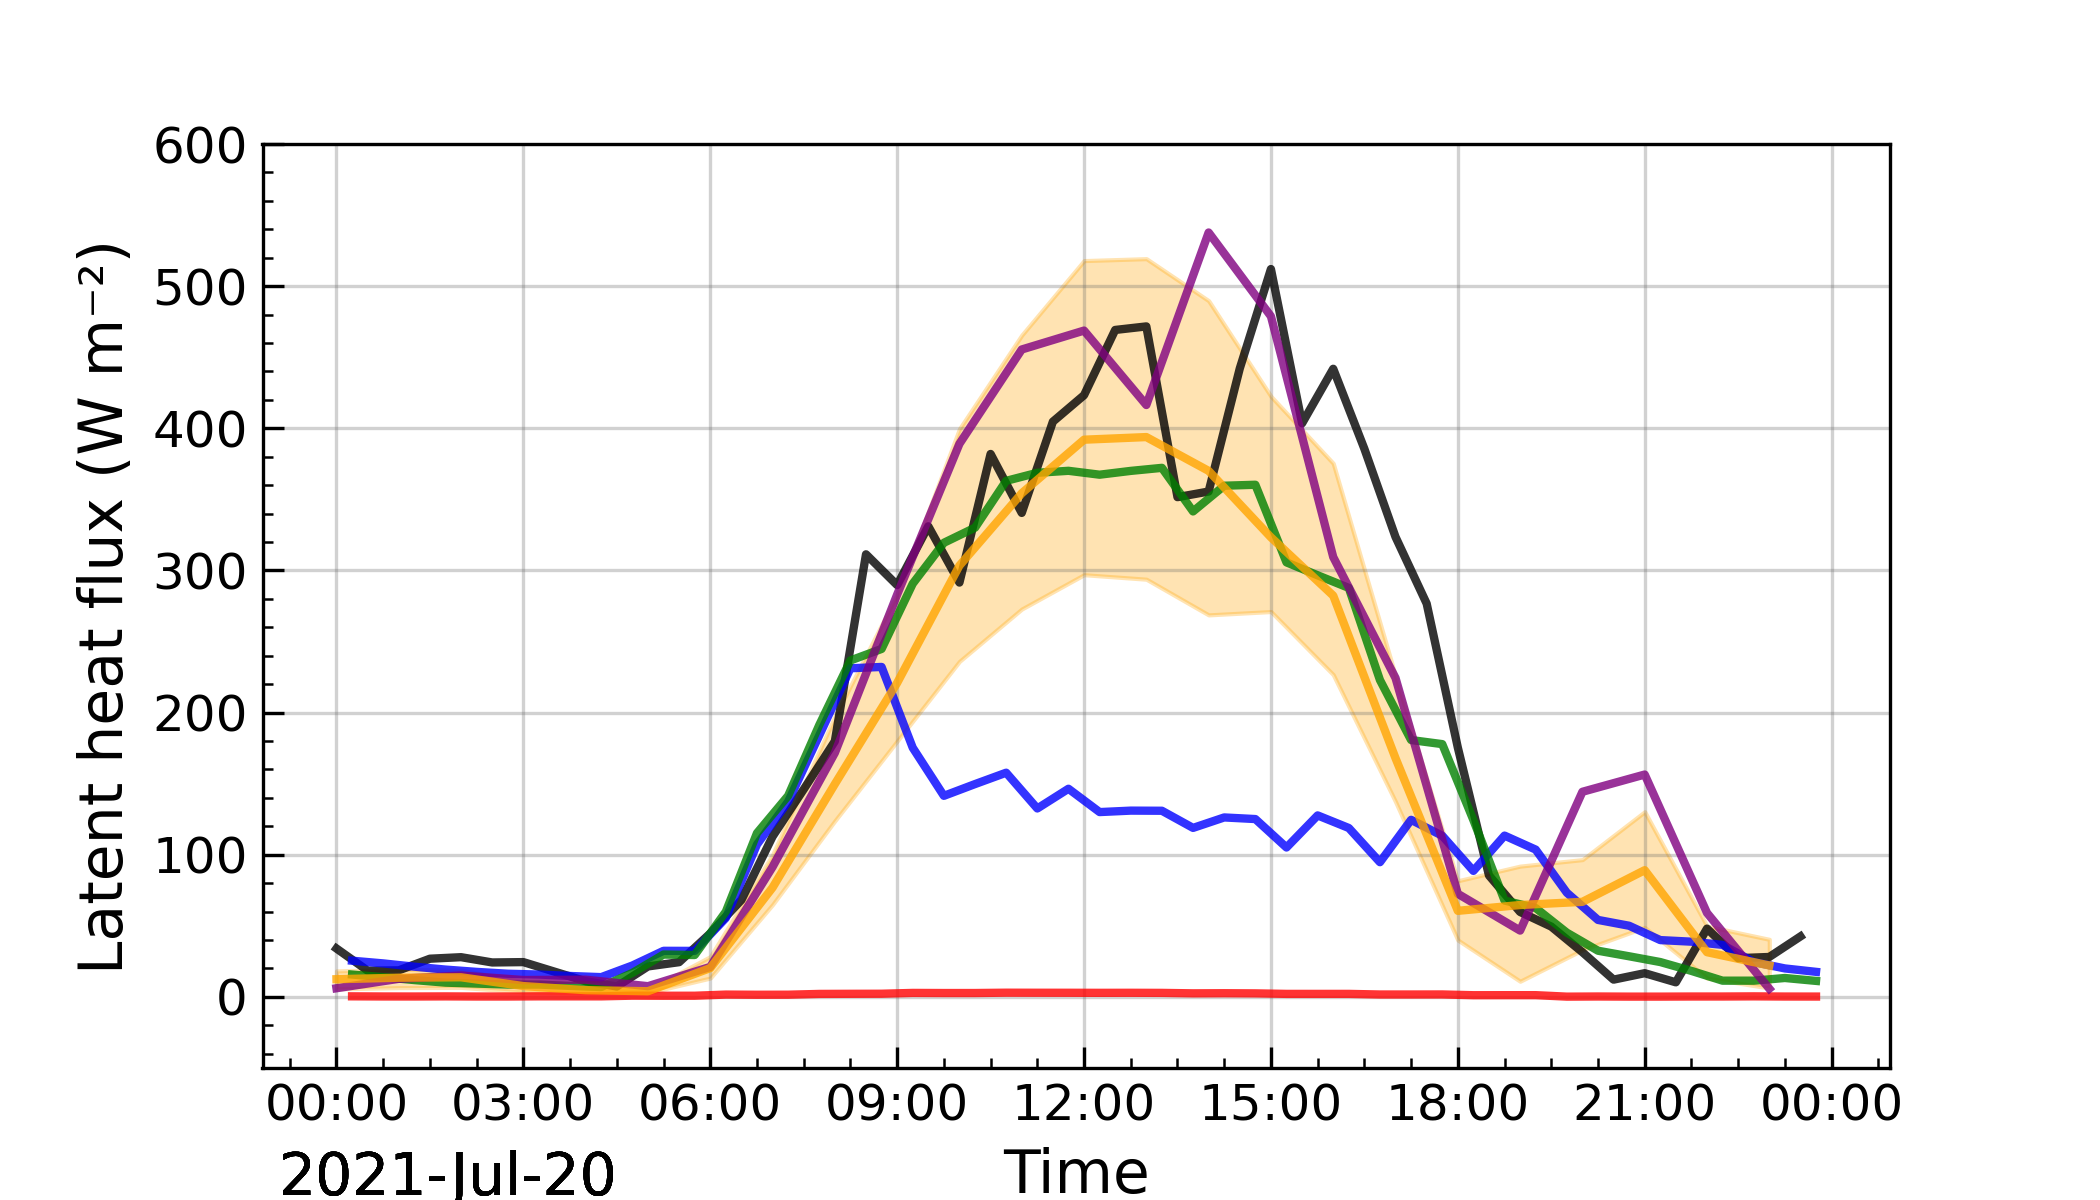
\includegraphics[width=\textwidth]{images/chap5/IOP_TS/TS_2021-07-20_cendrosa_flat.png}
        \end{subfigure} \\
        \begin{subfigure}[t]{0.5\textwidth}
            \caption{}
            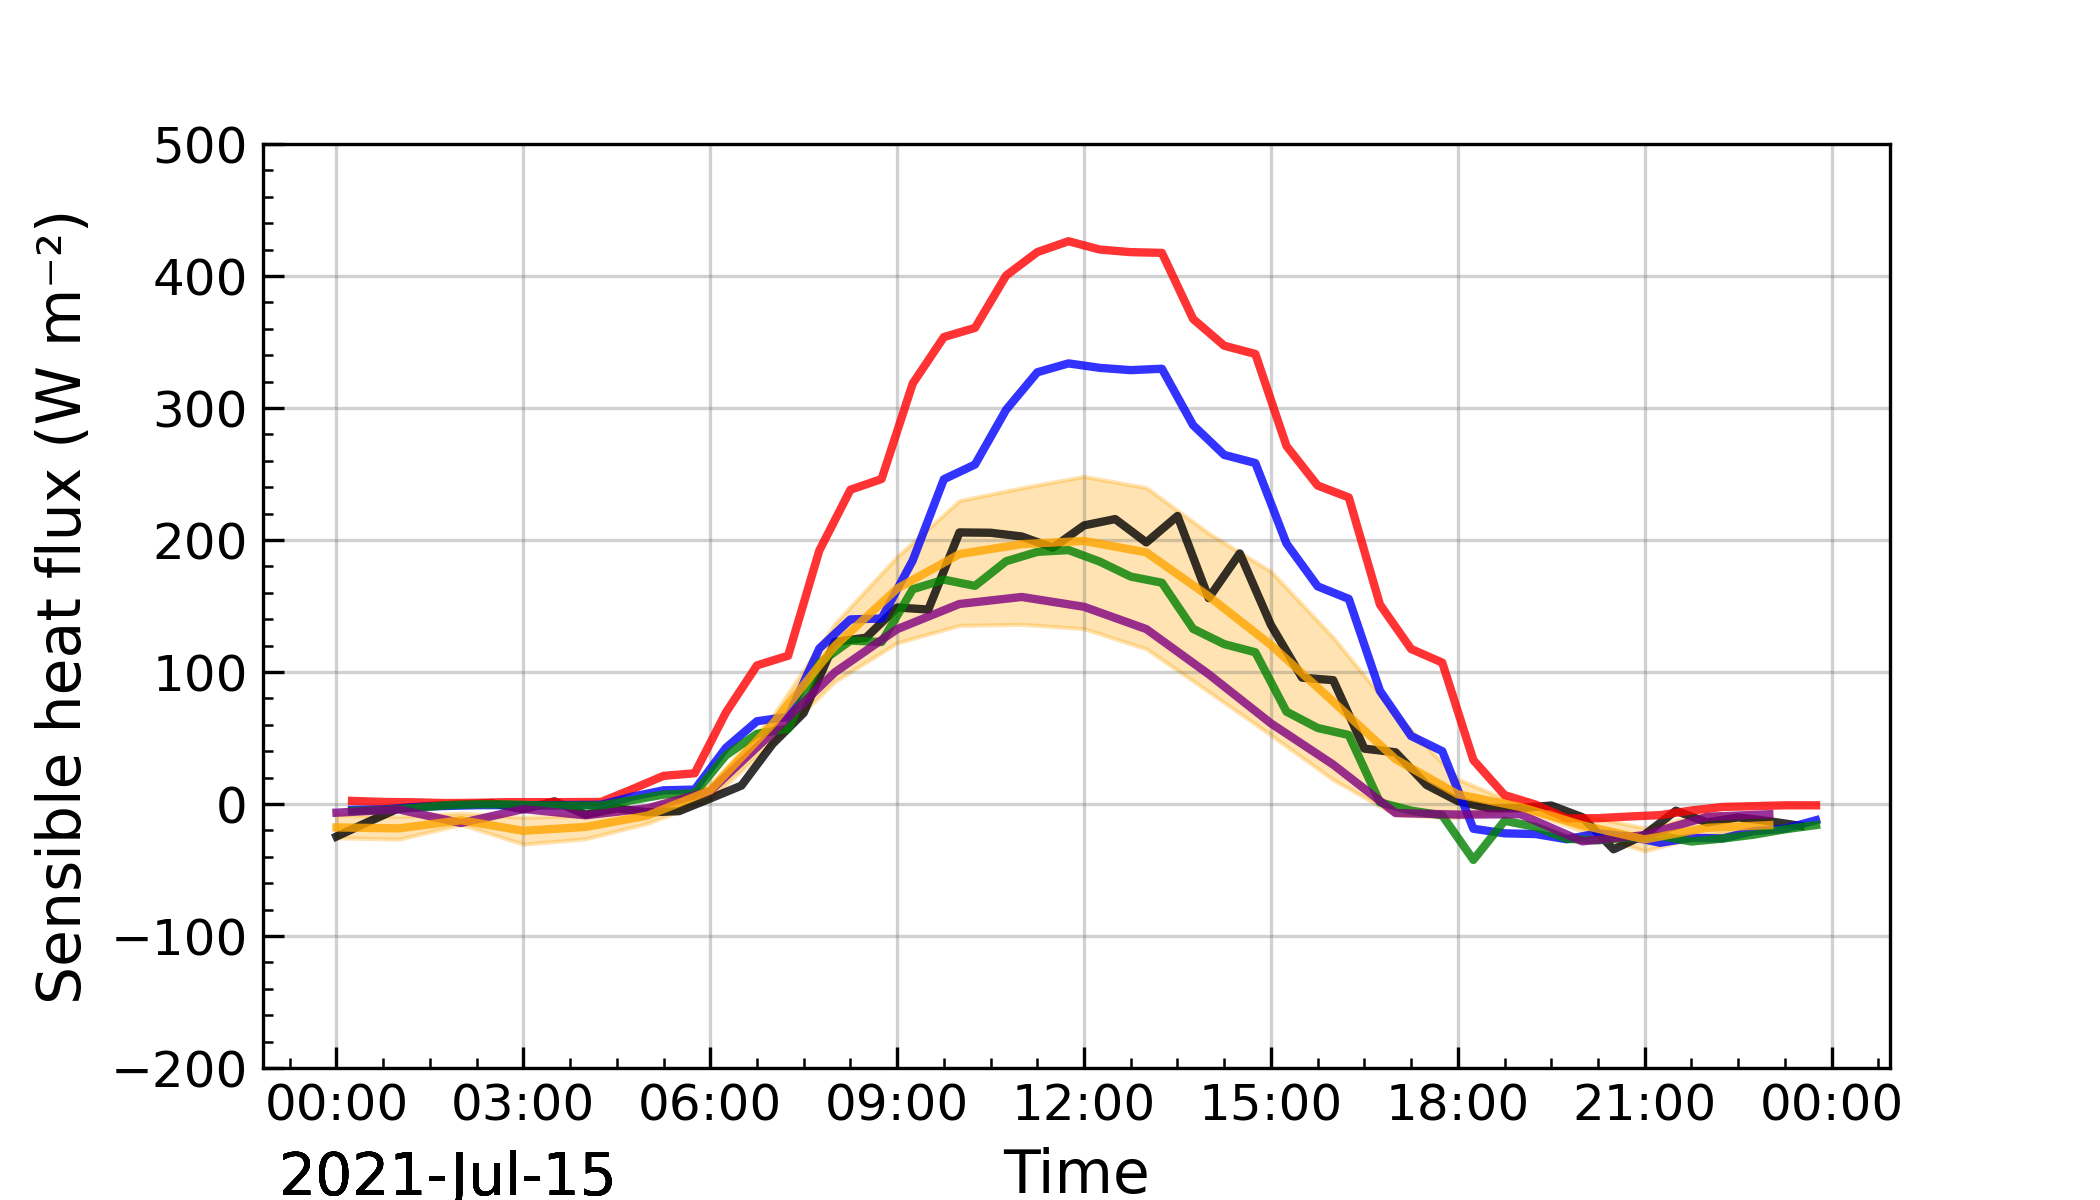
\includegraphics[width=\textwidth]{images/chap5/IOP_TS/TS_2021-07-15_cendrosa_sens.png}
        \end{subfigure} &
        \begin{subfigure}[t]{0.5\textwidth}
            \caption{}
            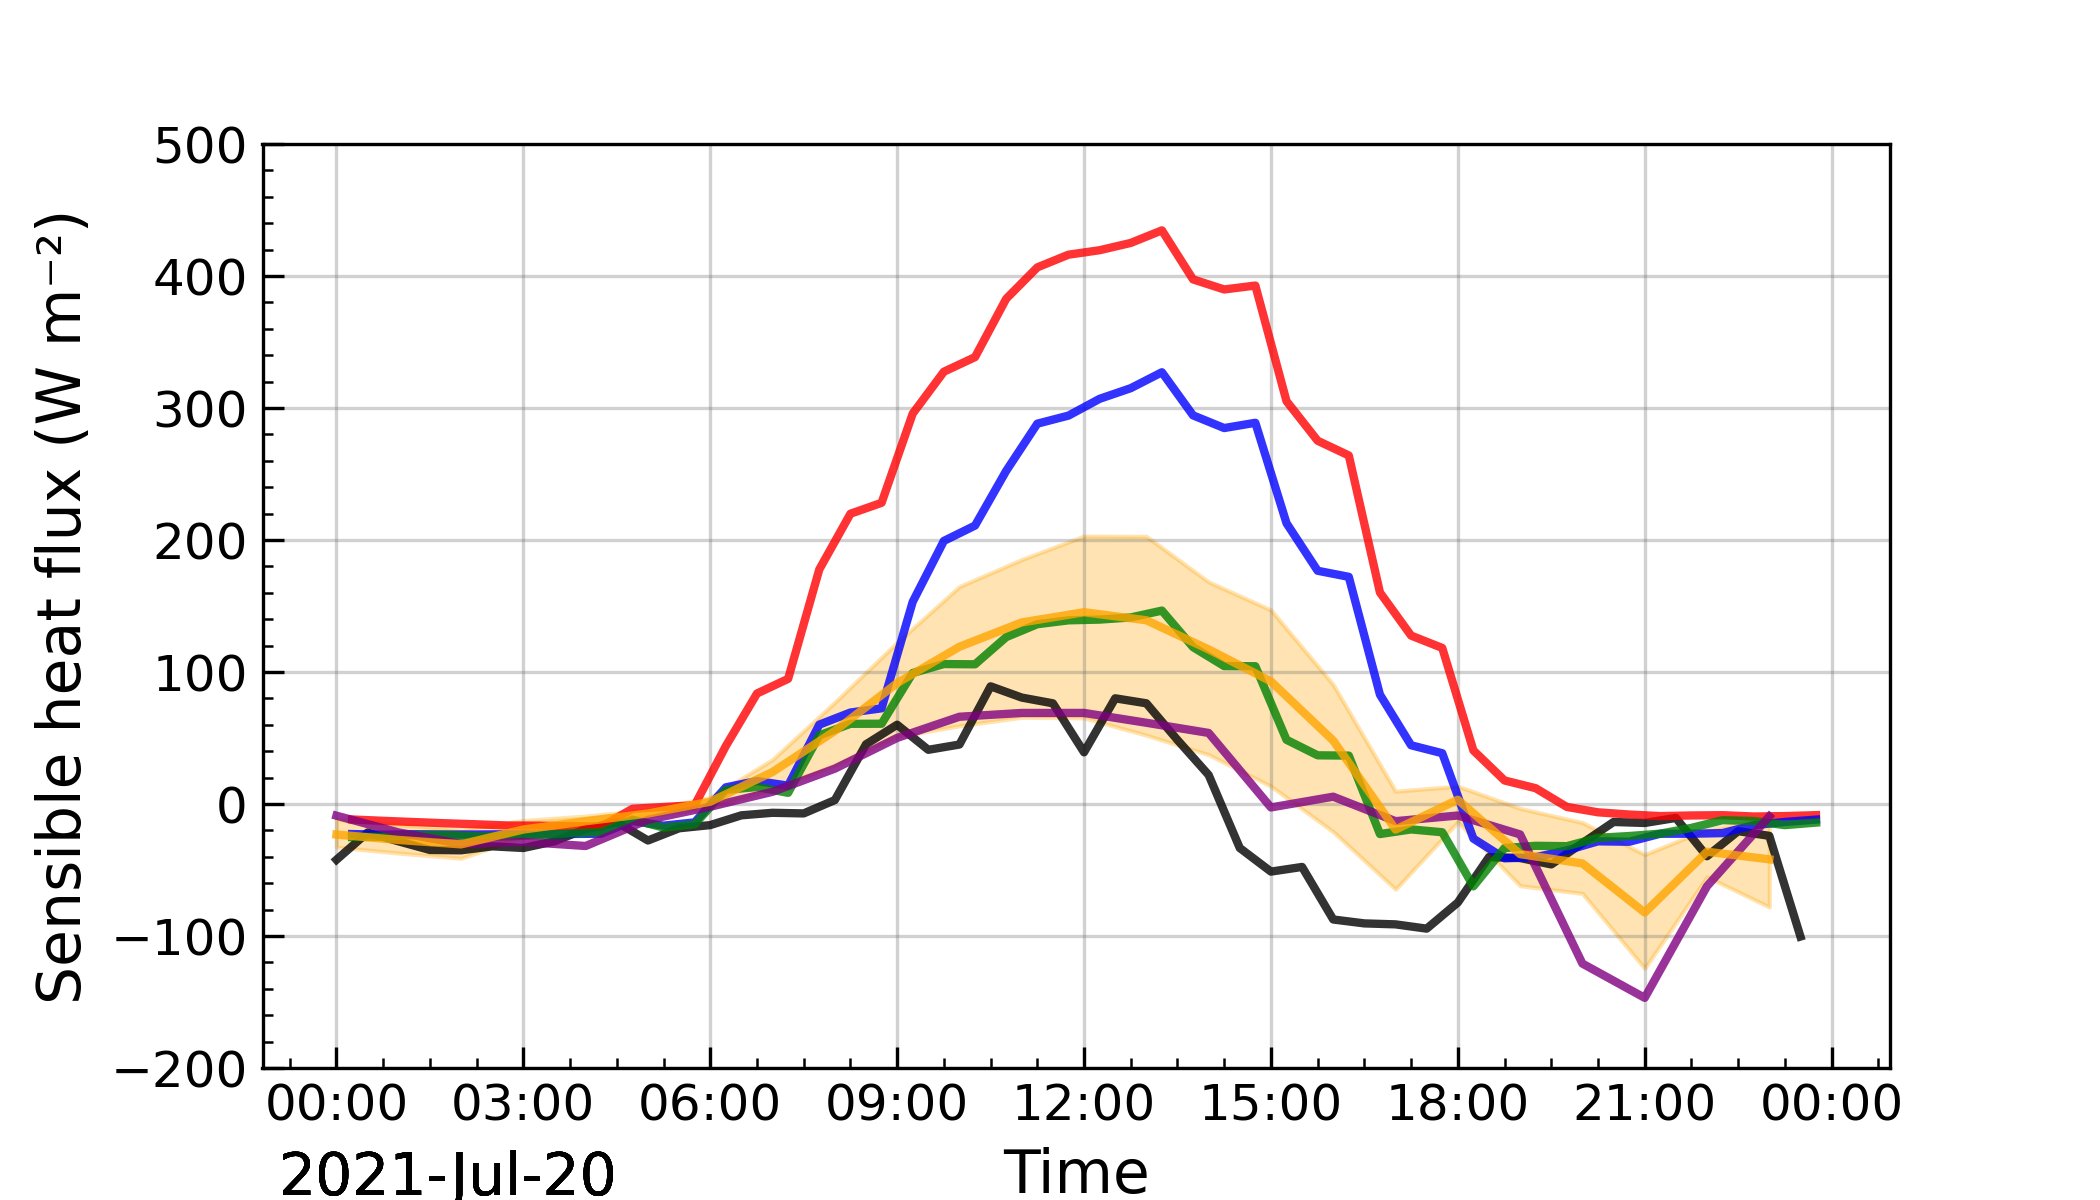
\includegraphics[width=\textwidth]{images/chap5/IOP_TS/TS_2021-07-20_cendrosa_sens.png}
        \end{subfigure} \\
    \end{tabular}
    \caption{}
    \label{fig:iop_days_TS_energy}
\end{figure}

%Fig : surface variables Cendrosa
\begin{figure}[hbtp]
    \centering
    \begin{tabular}{cc}
        %t2m, q2m
        \begin{subfigure}[t]{0.5\textwidth}
            \caption{}
            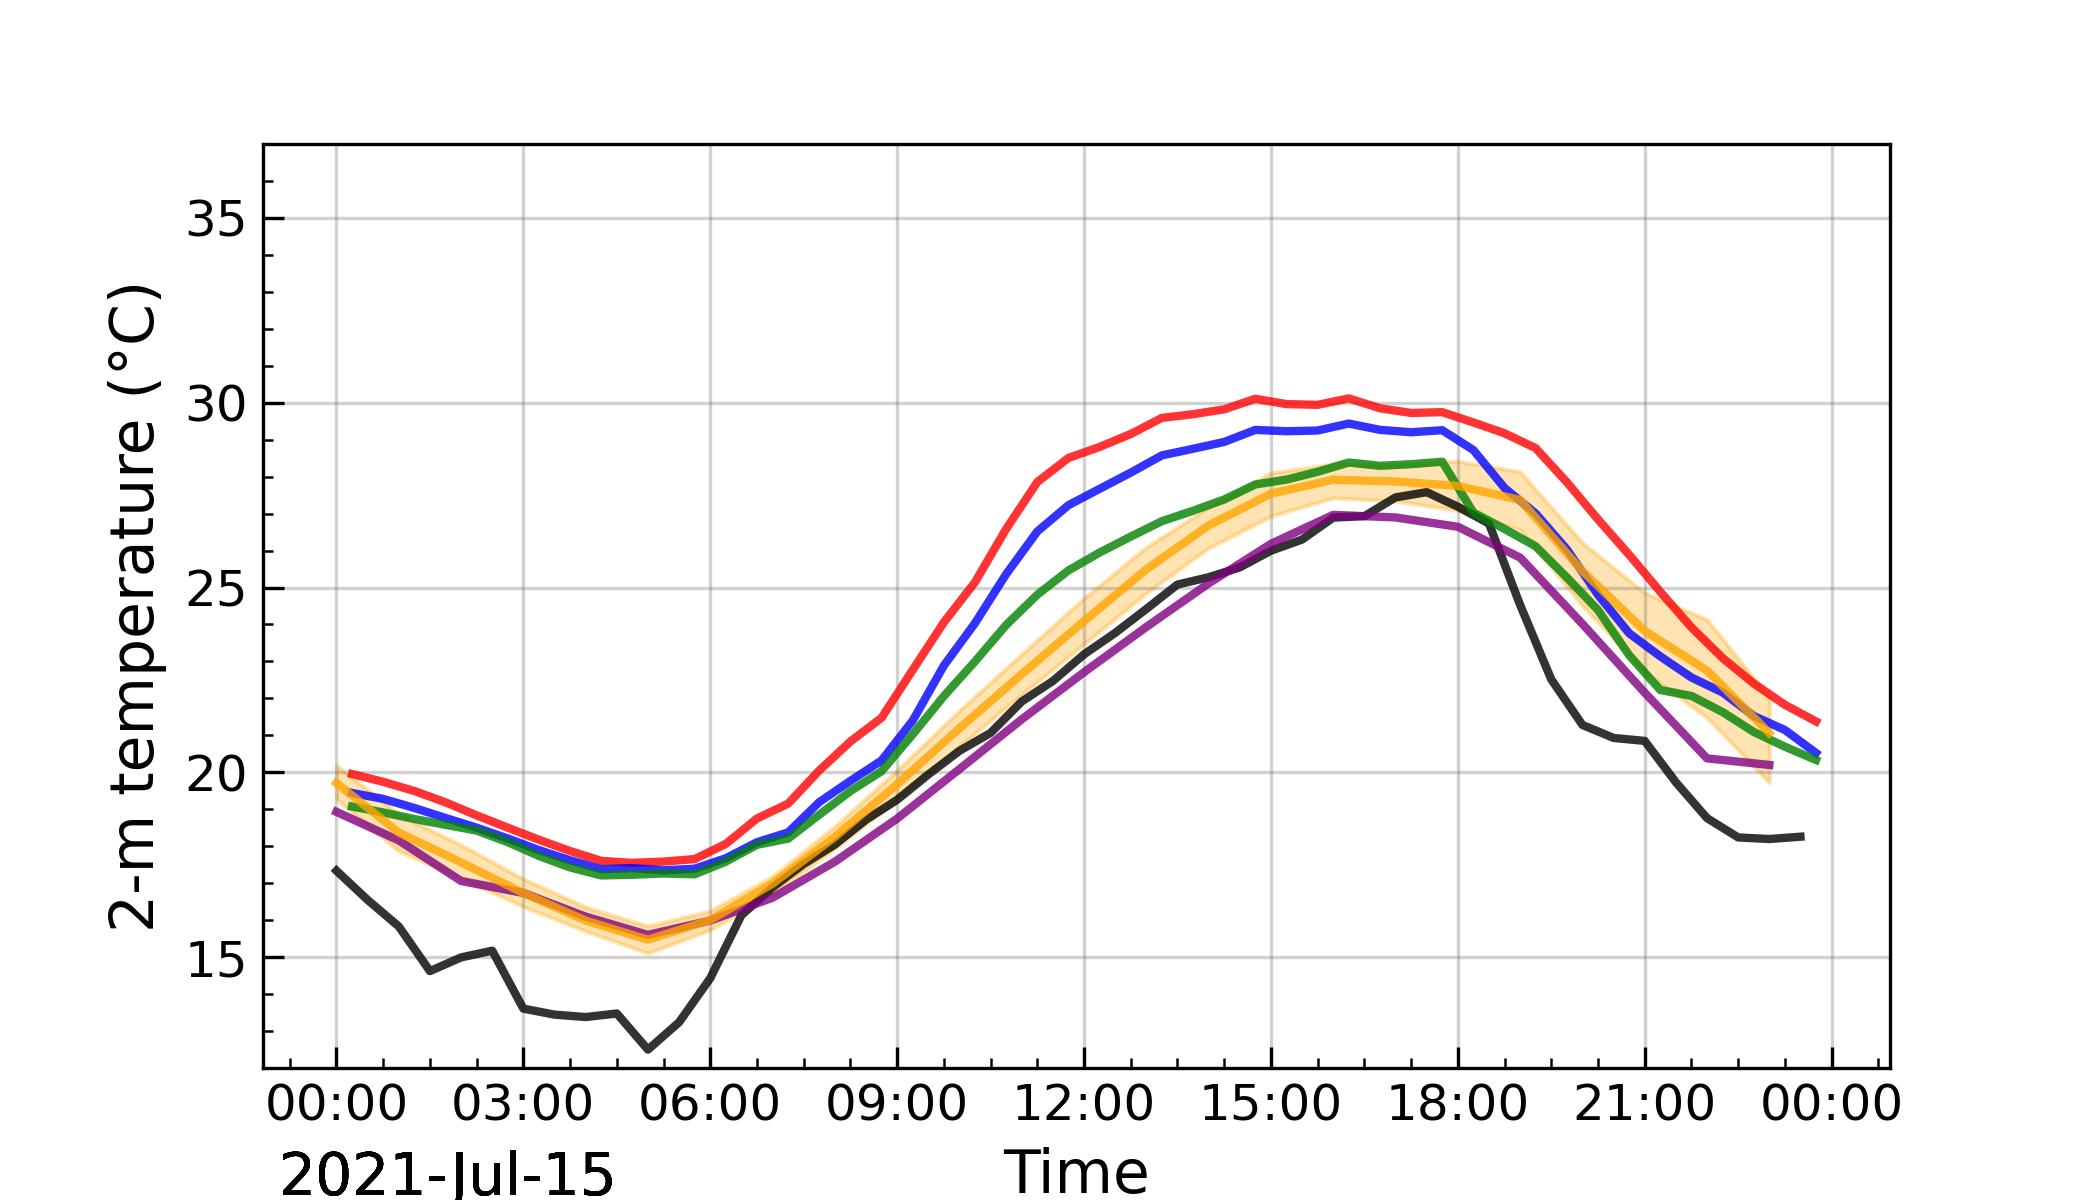
\includegraphics[width=\textwidth]{images/chap5/IOP_TS/TS_2021-07-15_cendrosa_t2m.png}
        \end{subfigure} &
        \begin{subfigure}[t]{0.5\textwidth}
            \caption{}
            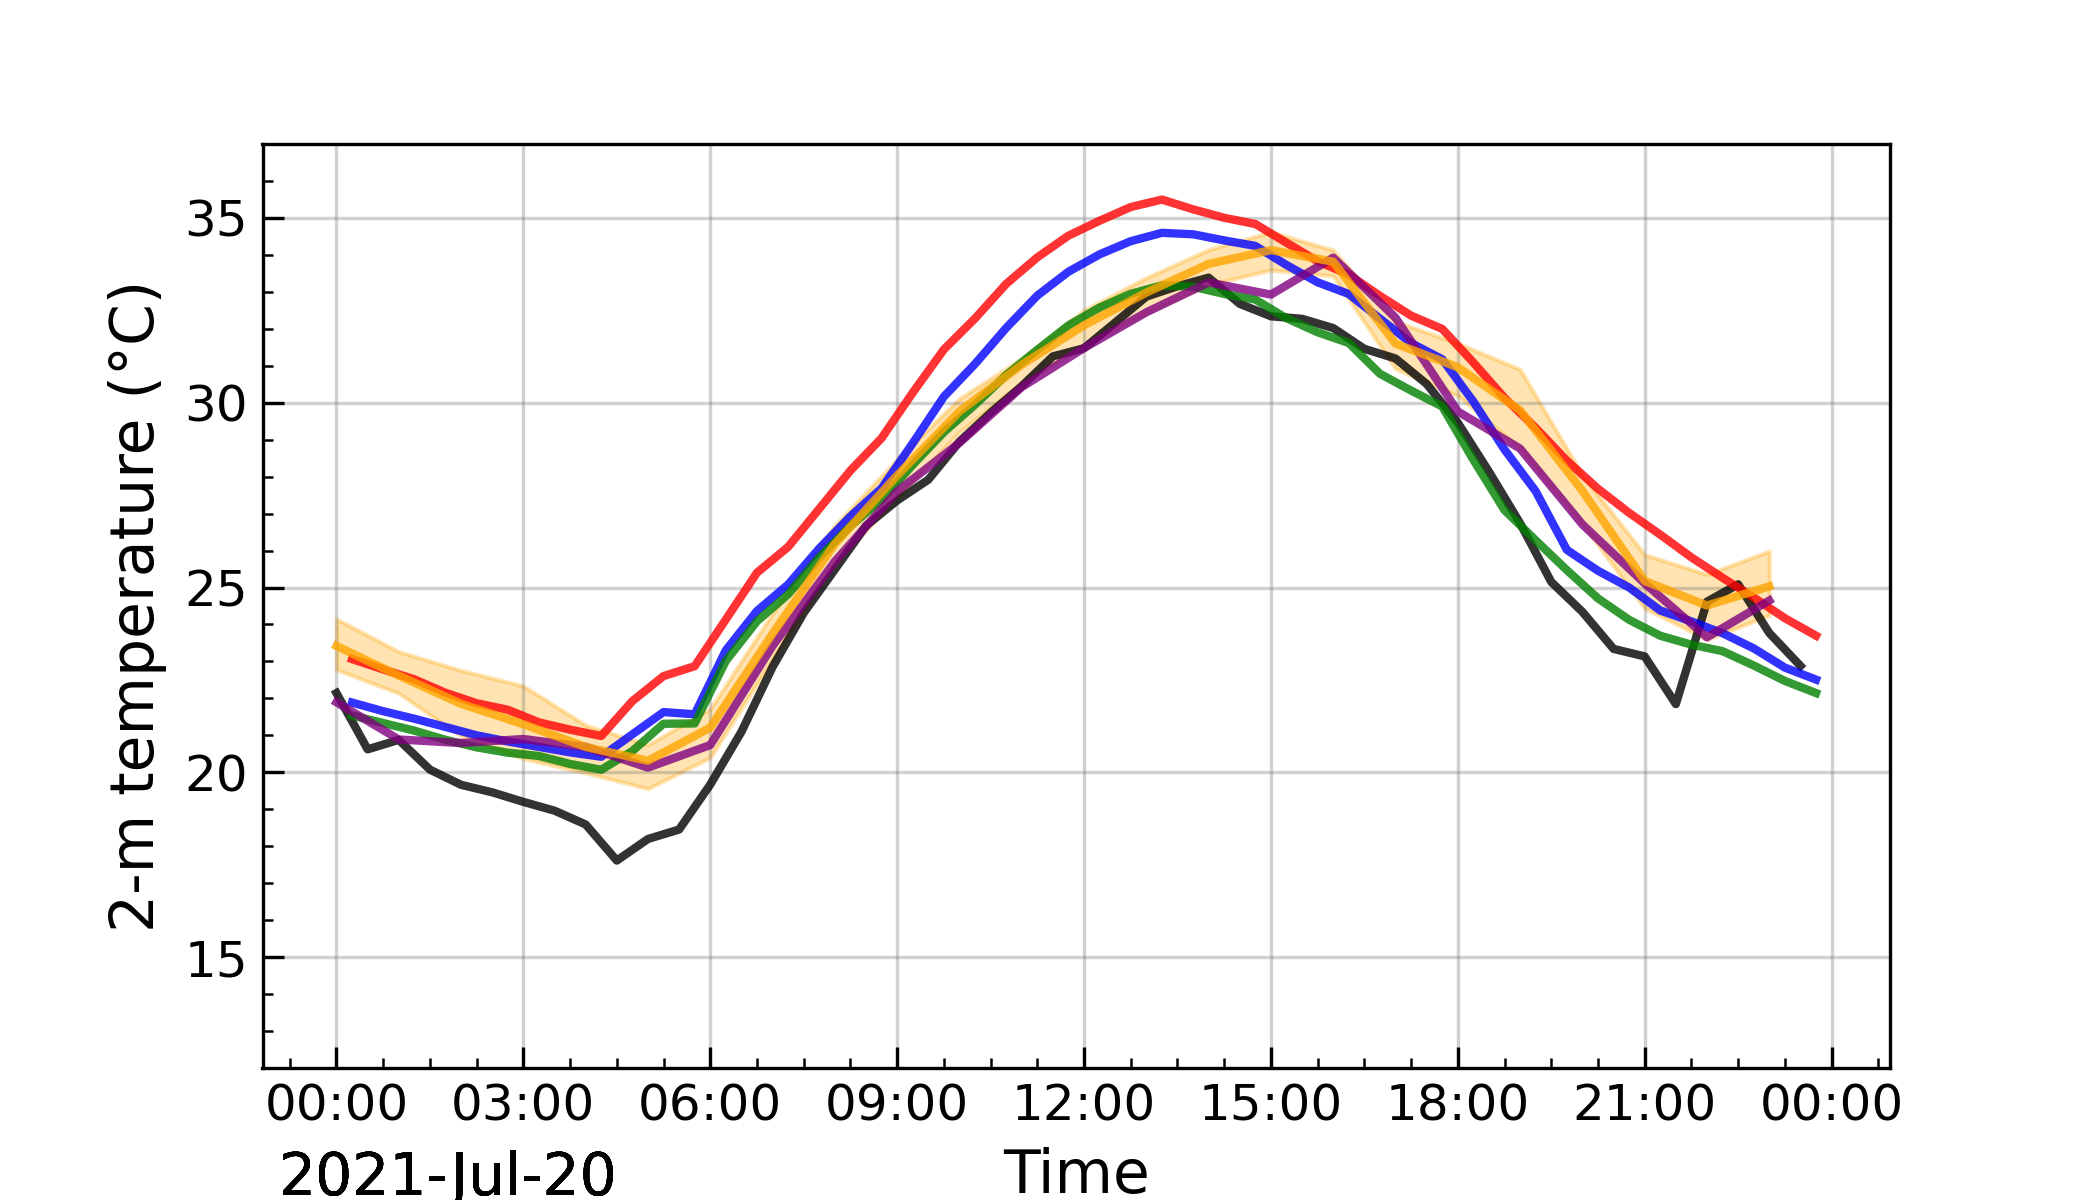
\includegraphics[width=\textwidth]{images/chap5/IOP_TS/TS_2021-07-20_cendrosa_t2m.png}
        \end{subfigure} \\
        \begin{subfigure}[t]{0.5\textwidth}
            \caption{}
            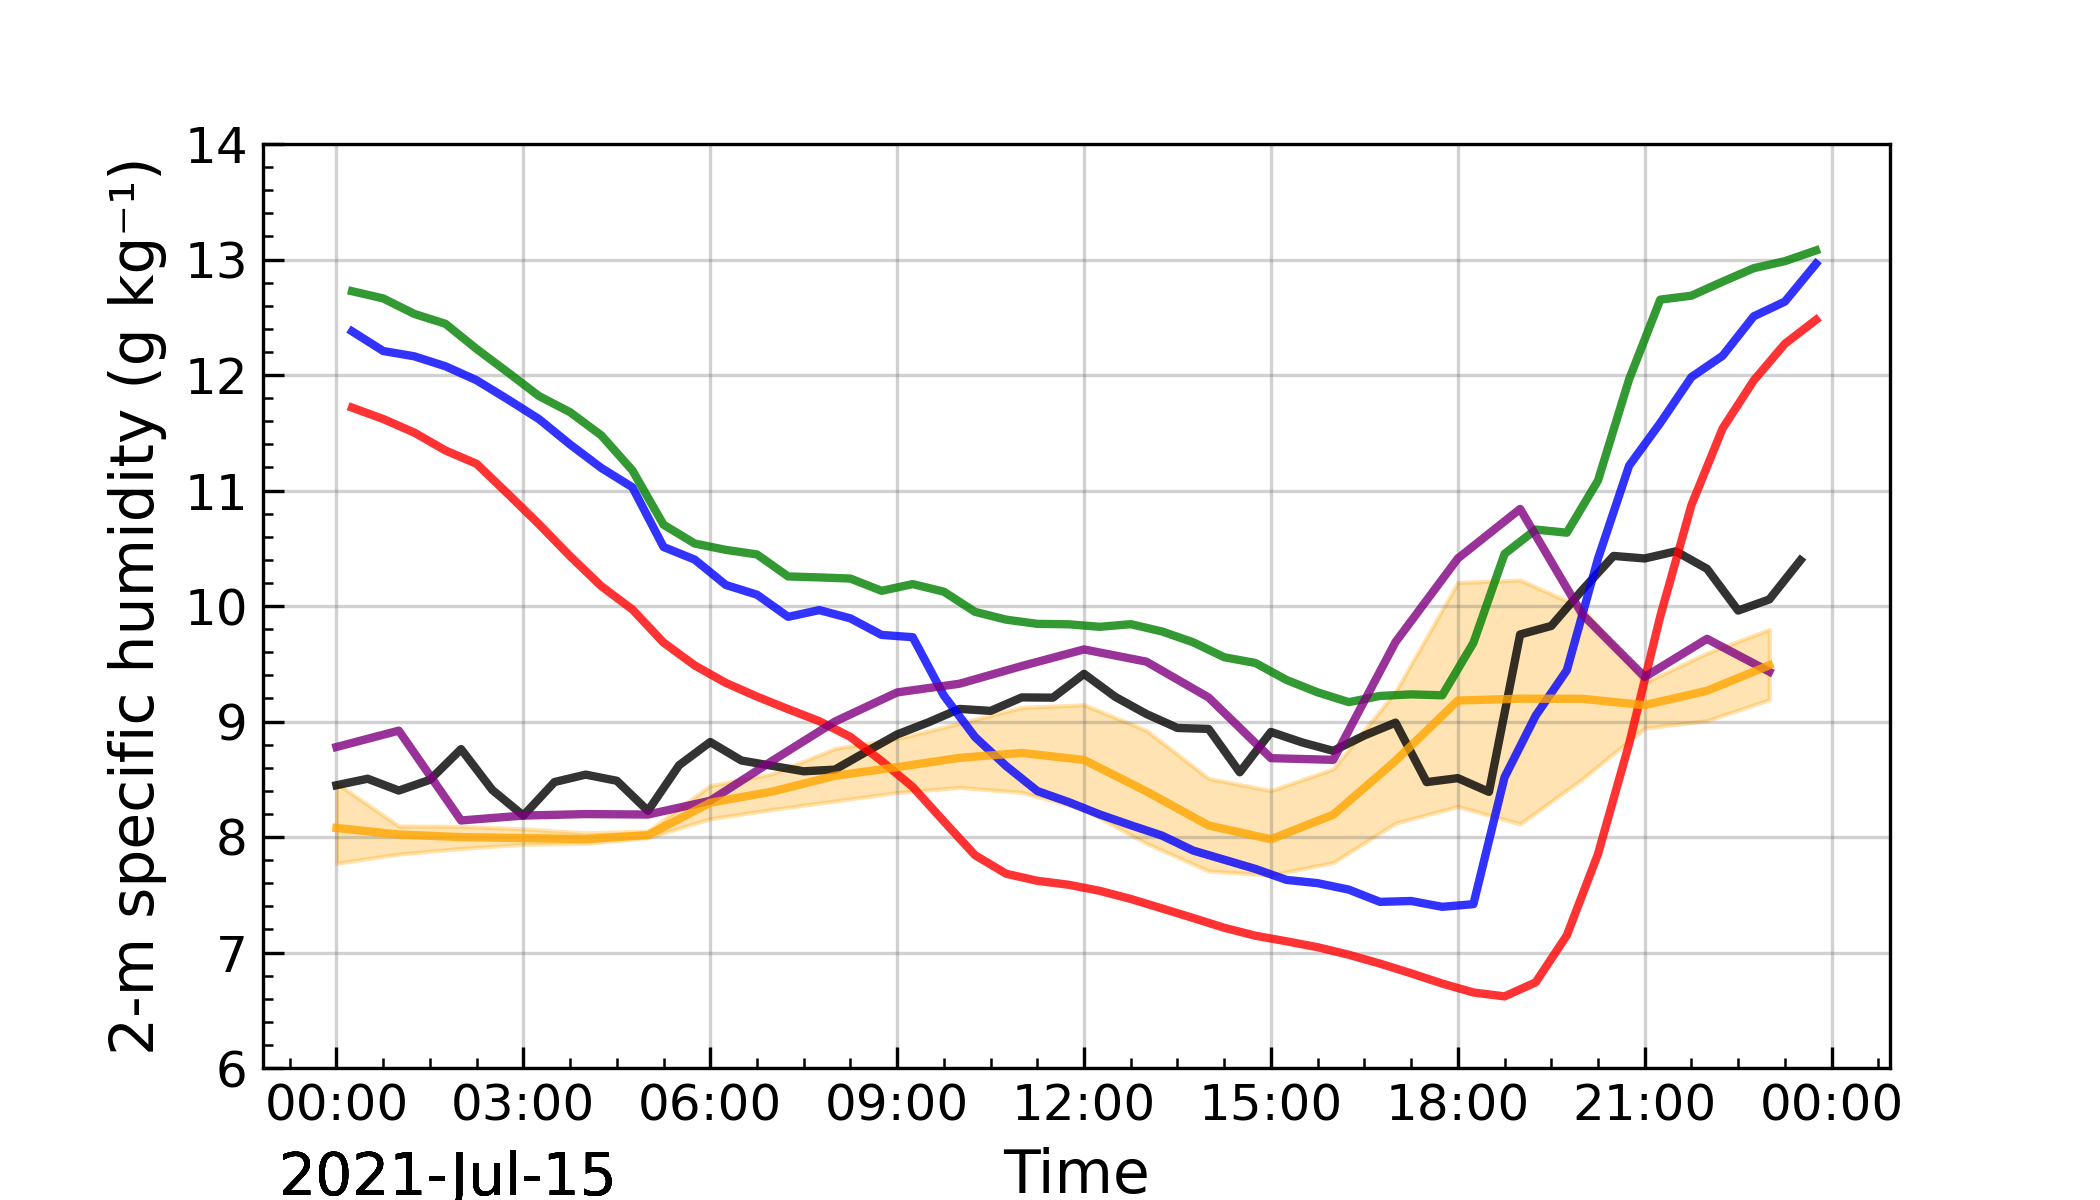
\includegraphics[width=\textwidth]{images/chap5/IOP_TS/TS_2021-07-15_cendrosa_q2m.png}
        \end{subfigure} &
        \begin{subfigure}[t]{0.5\textwidth}
            \caption{}
            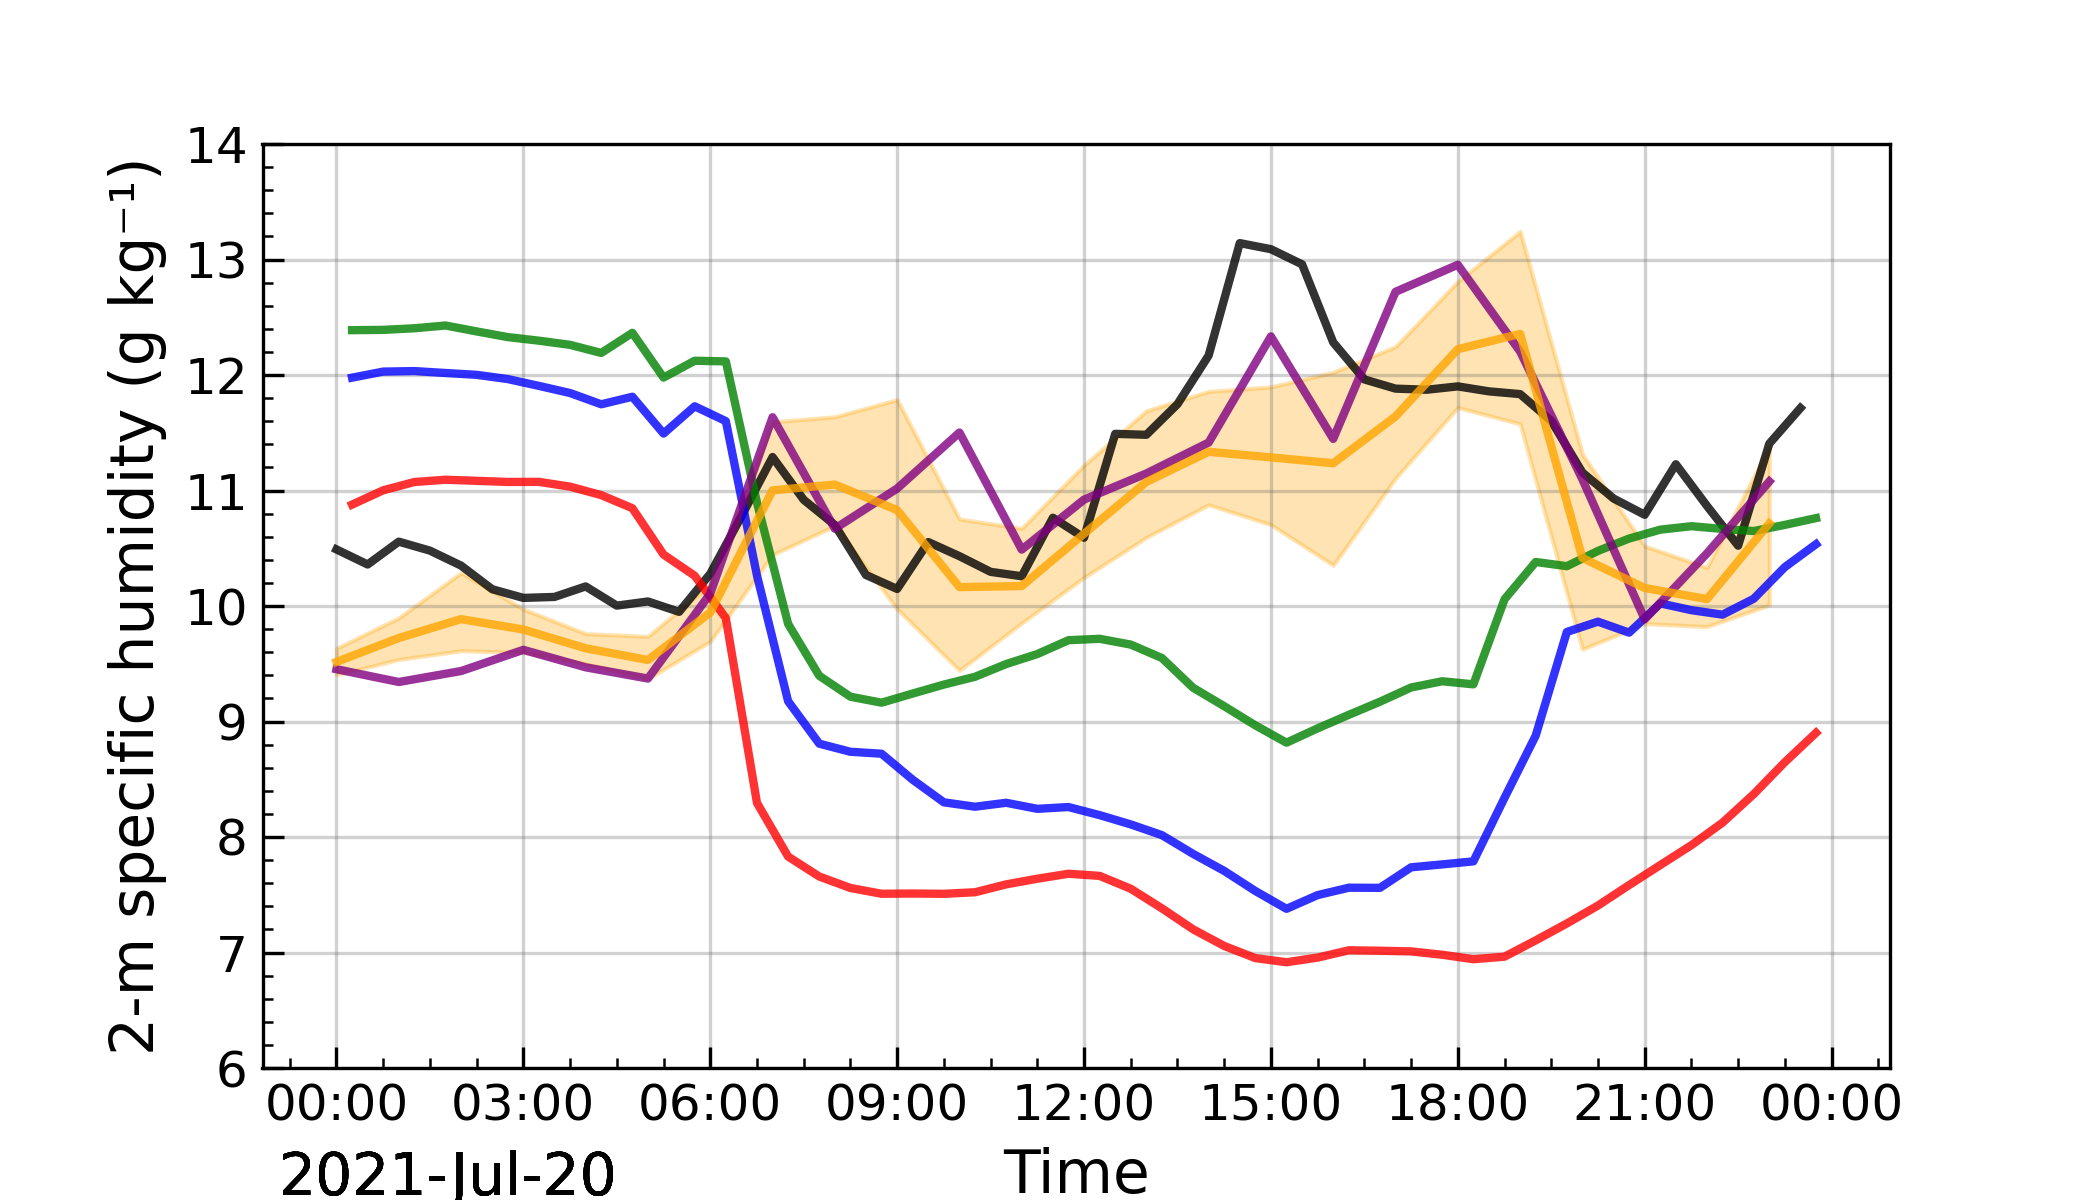
\includegraphics[width=\textwidth]{images/chap5/IOP_TS/TS_2021-07-20_cendrosa_q2m.png}
        \end{subfigure} \\

        %turb fluxes
        \begin{subfigure}[t]{0.5\textwidth}
            \caption{}
            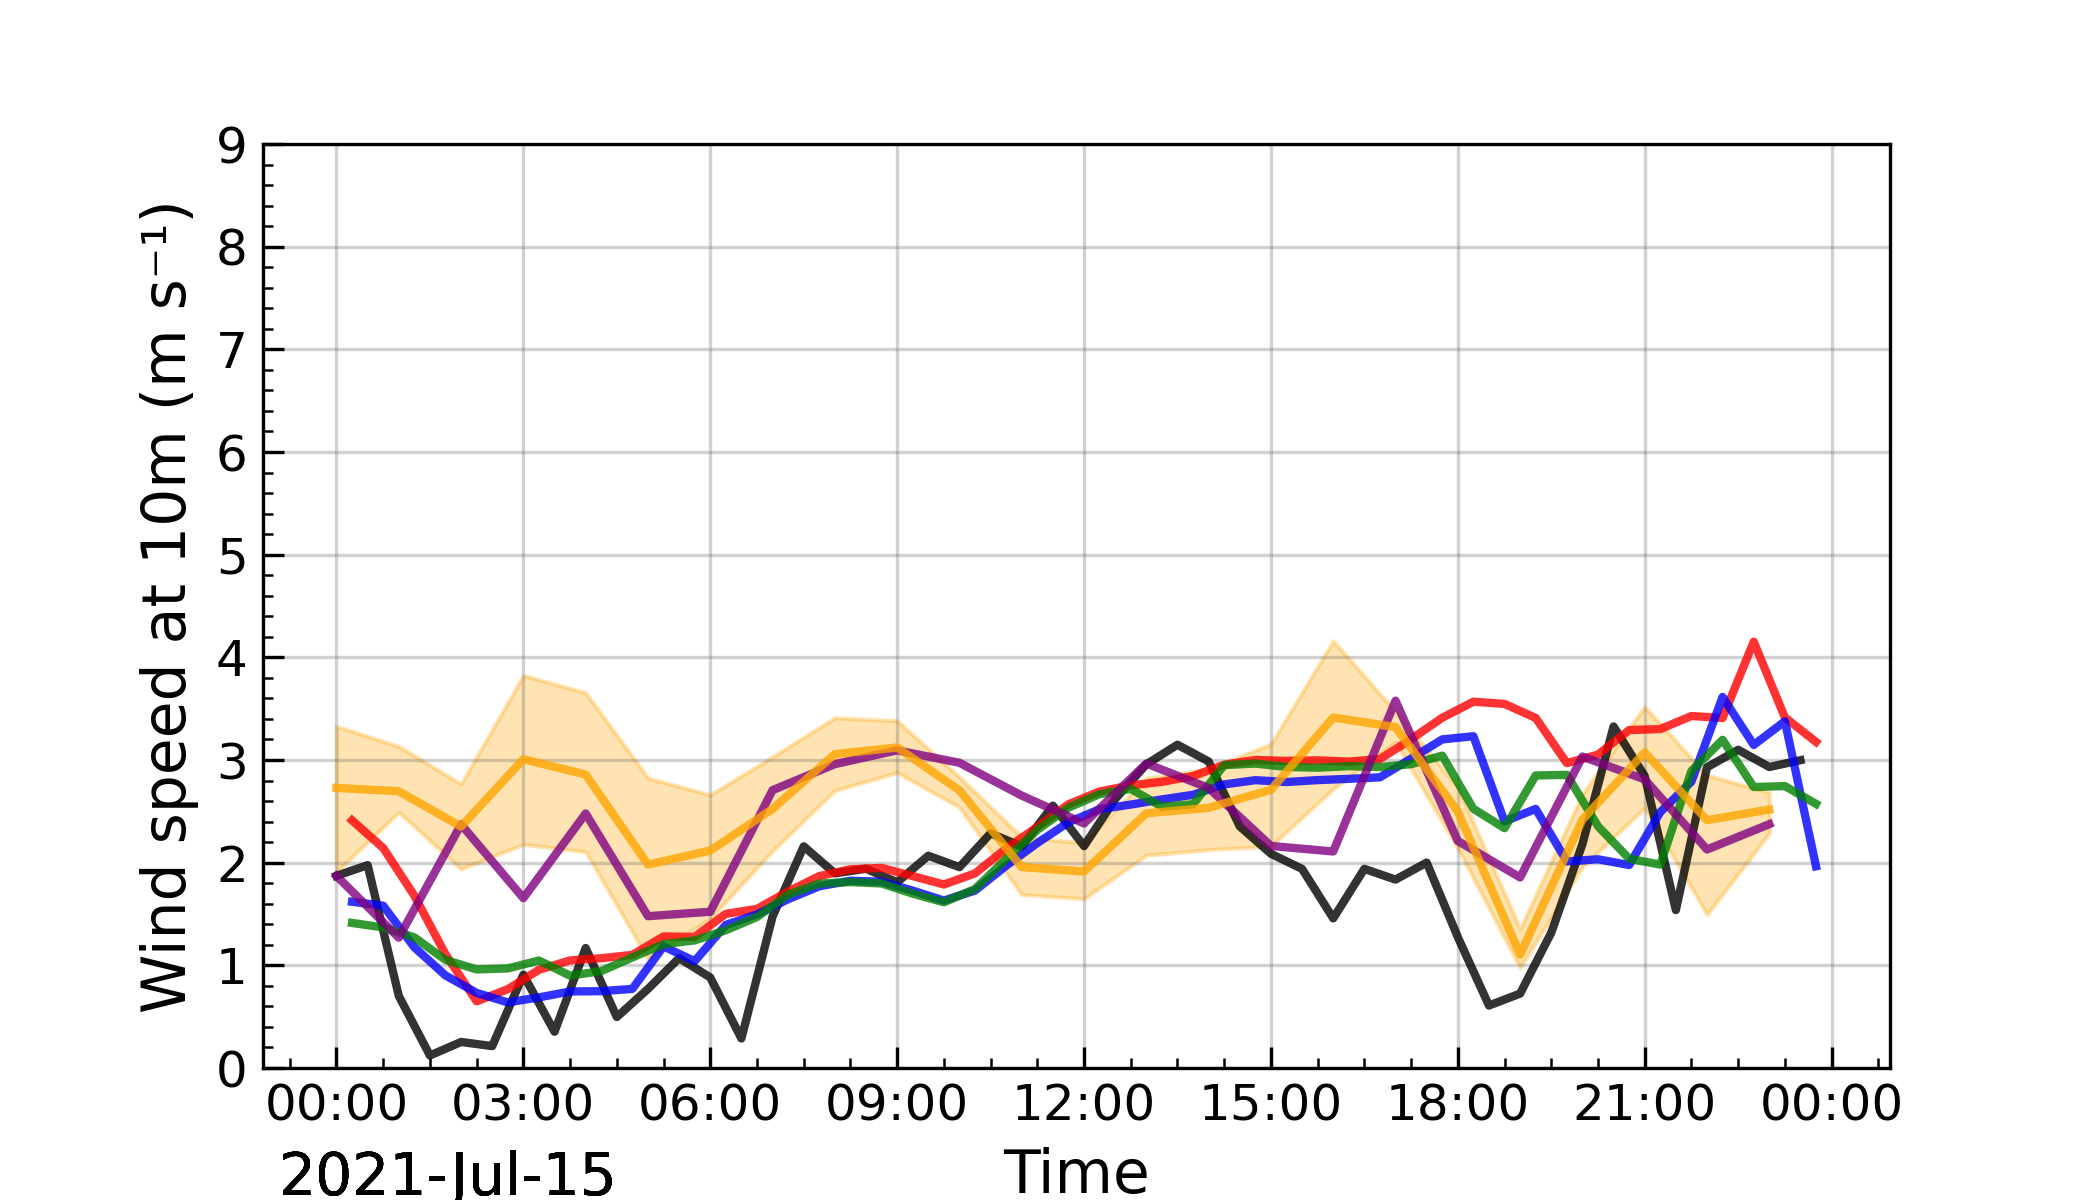
\includegraphics[width=\textwidth]{images/chap5/IOP_TS/TS_2021-07-15_cendrosa_wind_speed_10m.png}
        \end{subfigure} &
        \begin{subfigure}[t]{0.5\textwidth}
            \caption{}
            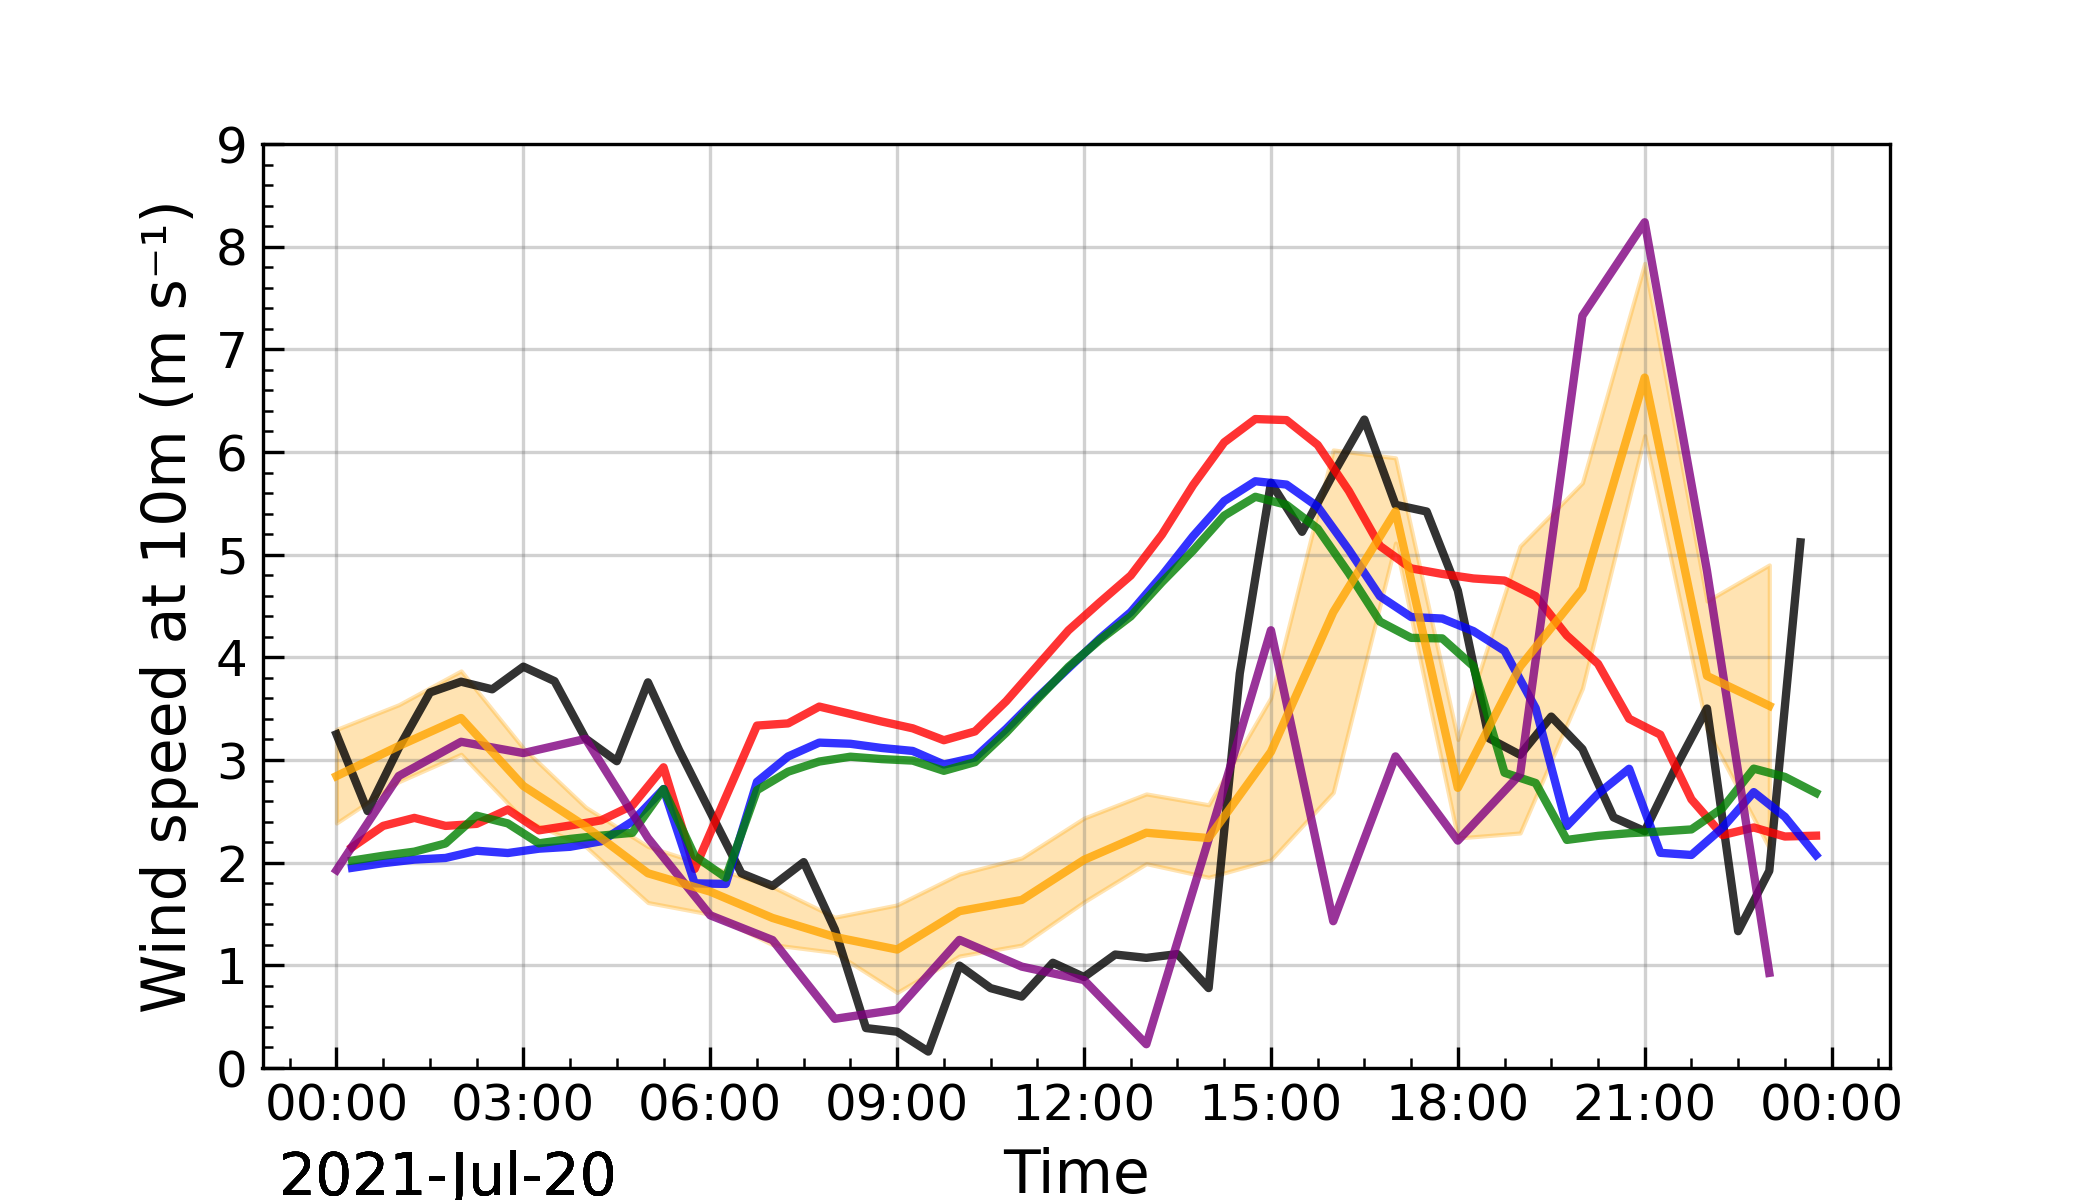
\includegraphics[width=\textwidth]{images/chap5/IOP_TS/TS_2021-07-20_cendrosa_wind_speed_10m.png}
        \end{subfigure} \\
        \begin{subfigure}[t]{0.5\textwidth}
            \caption{}
            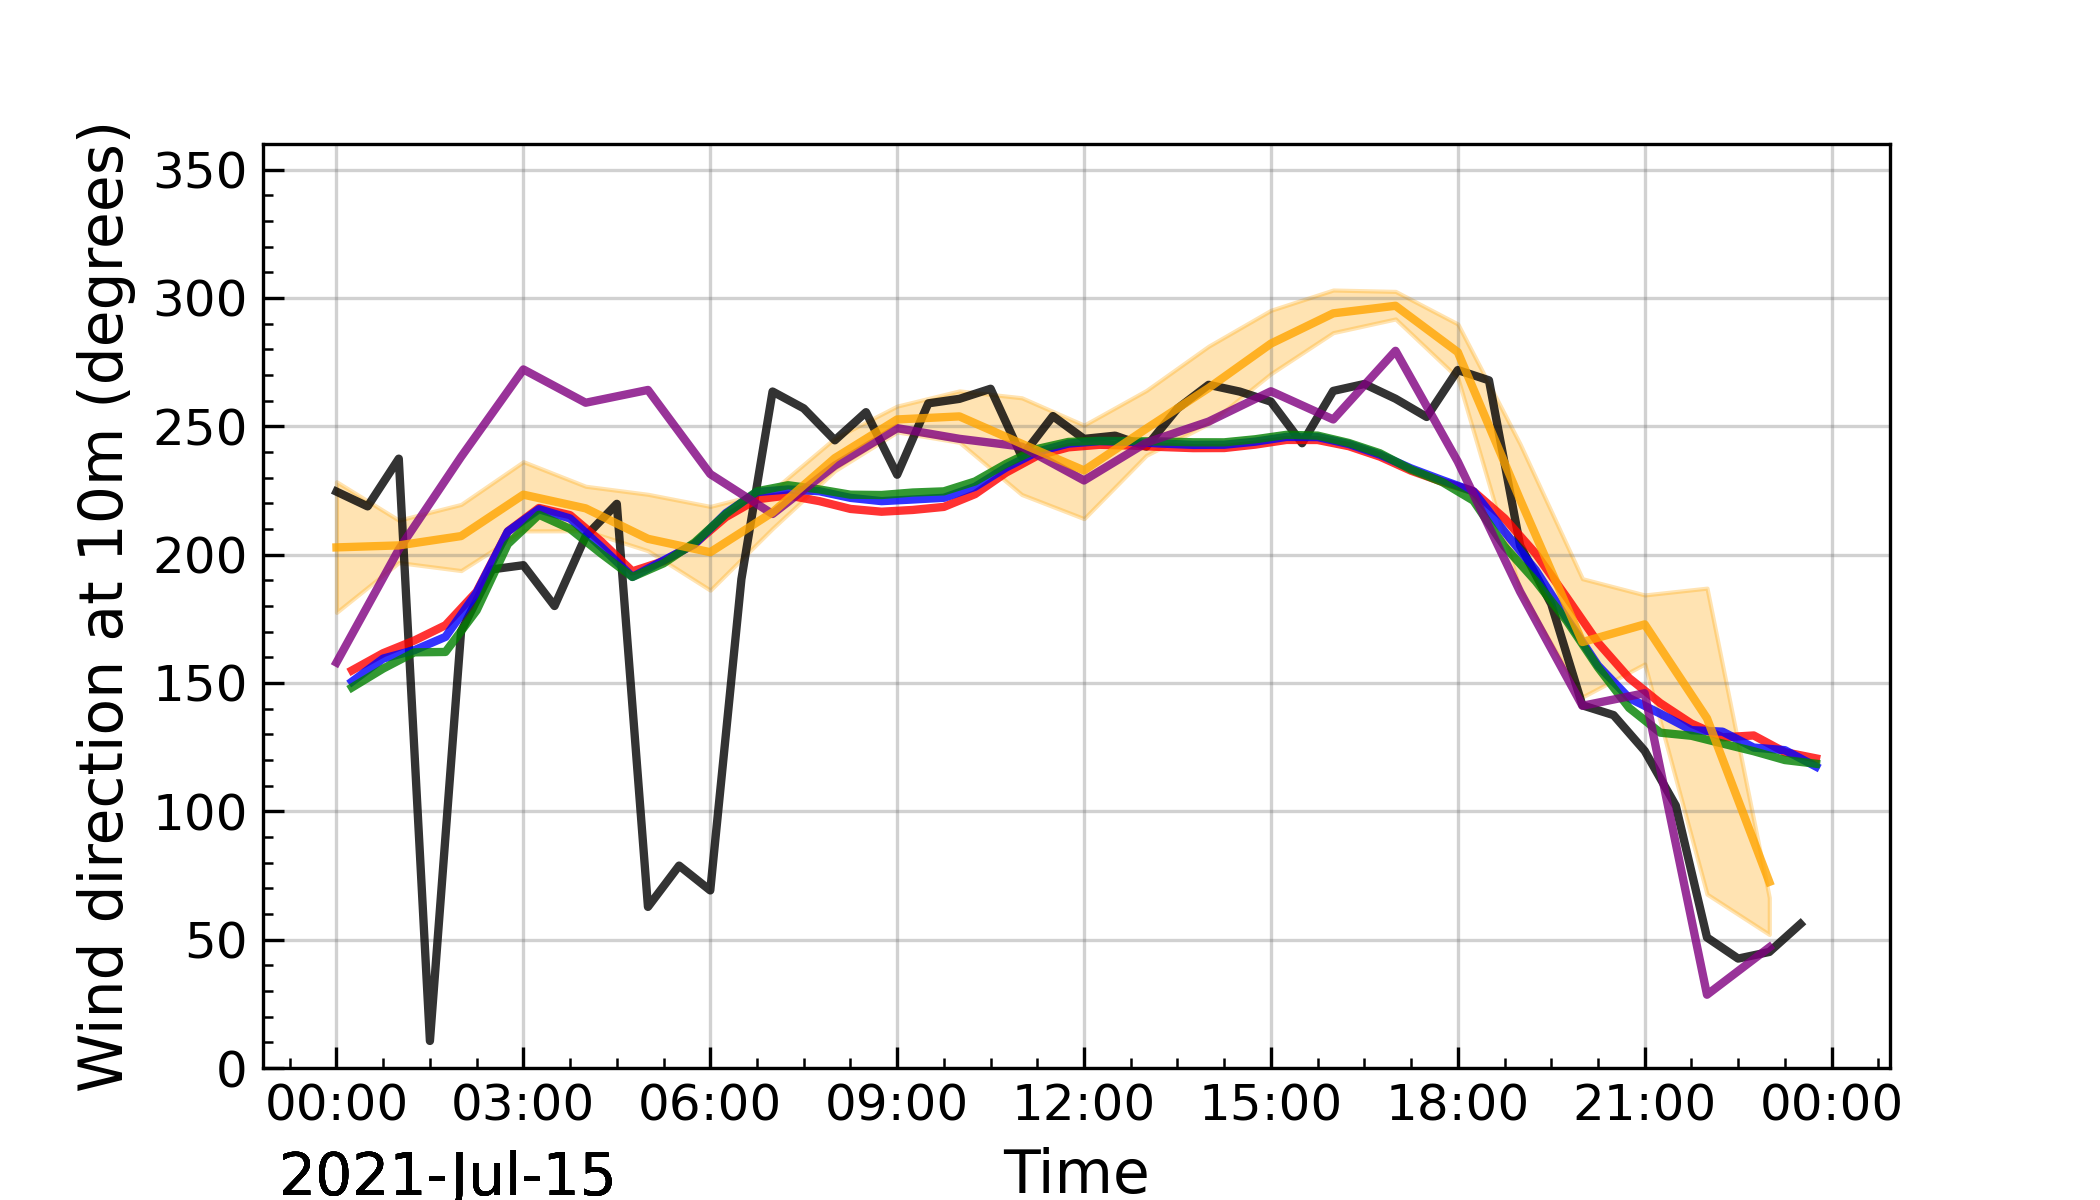
\includegraphics[width=\textwidth]{images/chap5/IOP_TS/TS_2021-07-15_cendrosa_wind_direction_10m.png}
        \end{subfigure} &
        \begin{subfigure}[t]{0.5\textwidth}
            \caption{}
            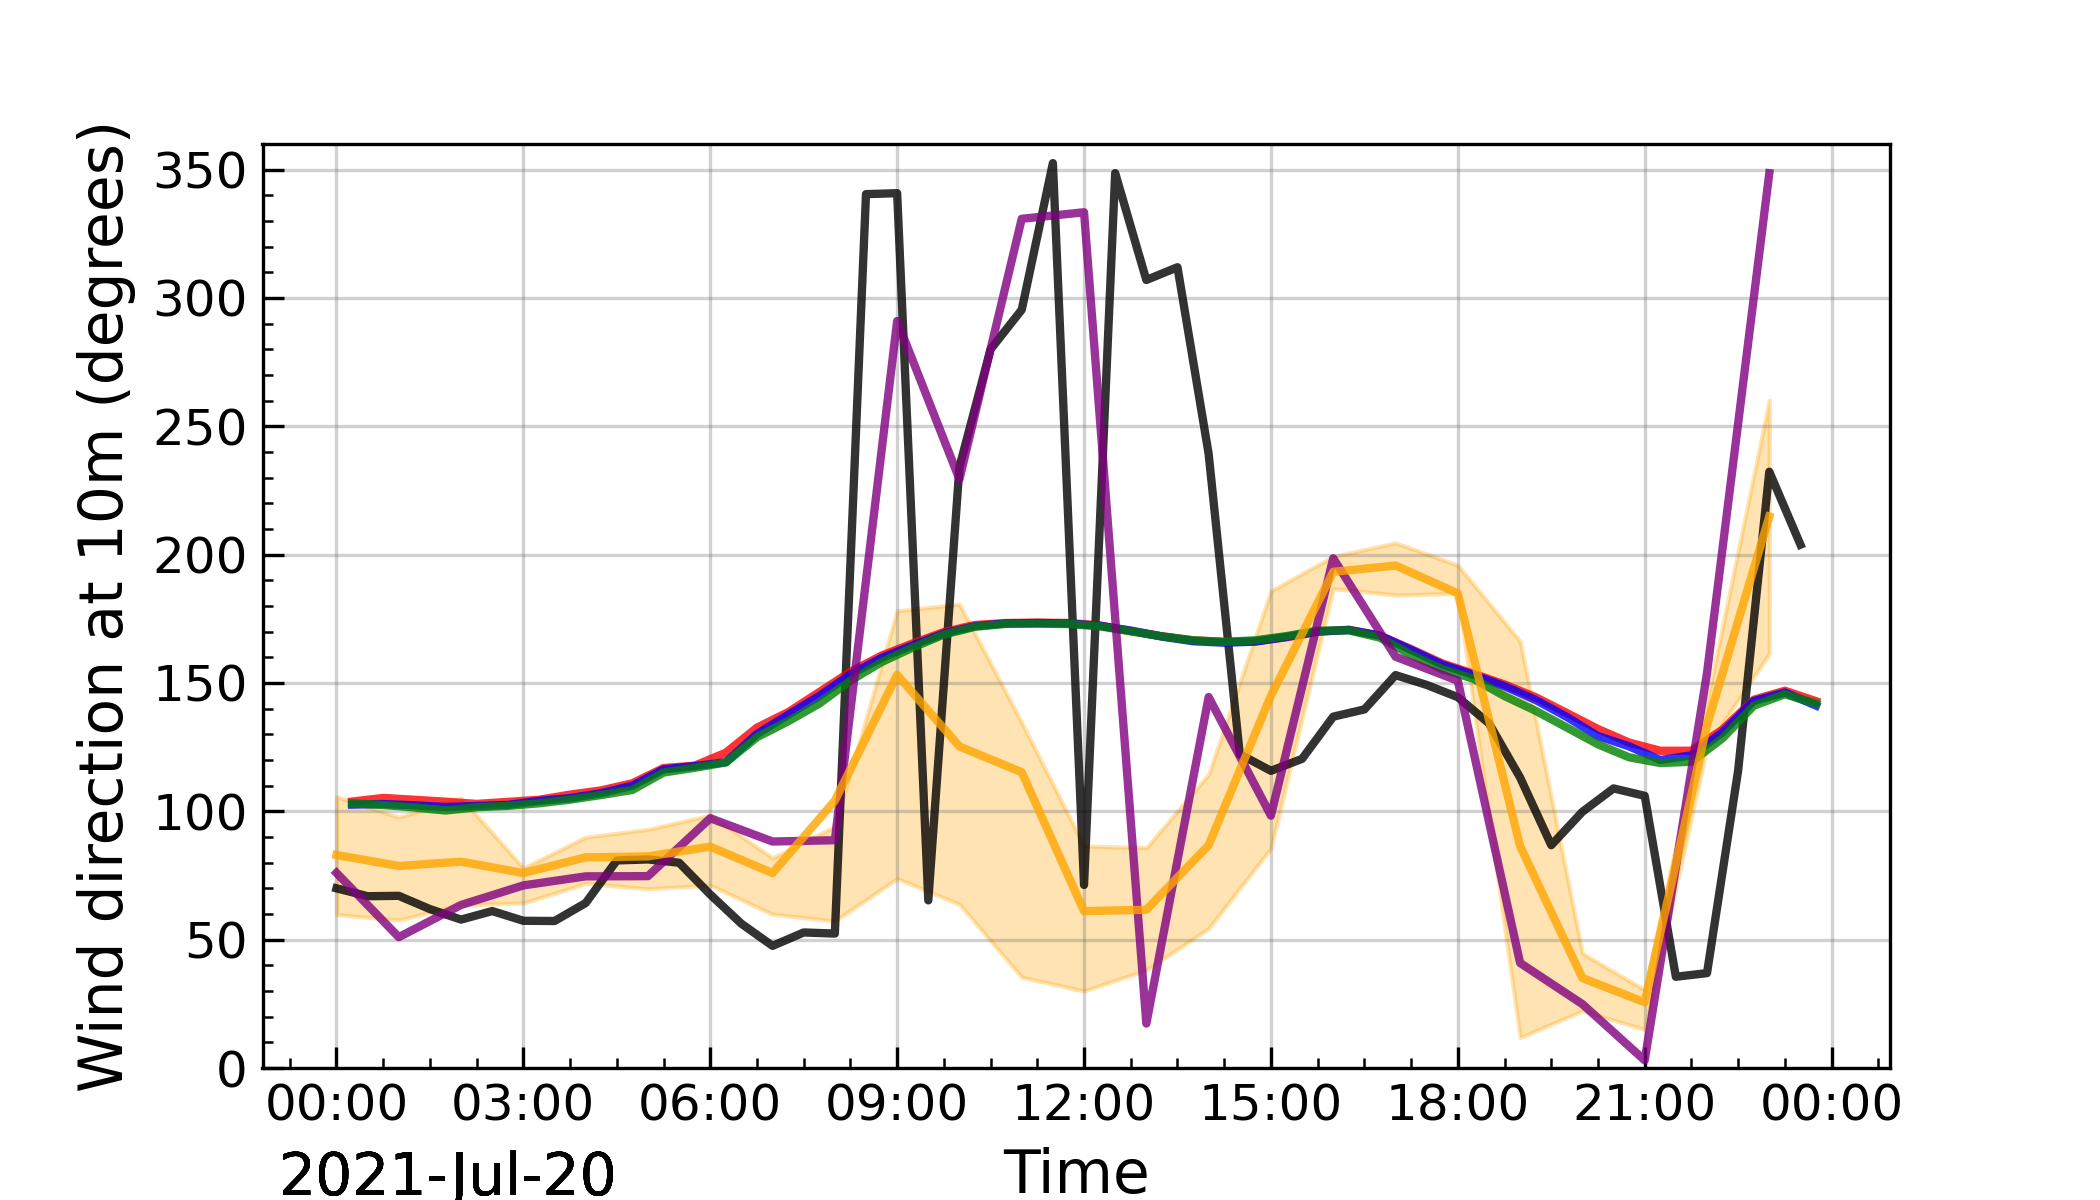
\includegraphics[width=\textwidth]{images/chap5/IOP_TS/TS_2021-07-20_cendrosa_wind_direction_10m.png}
        \end{subfigure} \\
    \end{tabular}
    \caption{}
    \label{fig:iop_days_TS_surfvars}
\end{figure}

%todo:figure of winds at 12UTC (10m and 850hPa) ideally mesoNH and LMDZ

\clearpage
\subsection{Vertical profiles at 12UTC}
%July 15th
%noirr : ABL too high in ICOLMDZ (also visible at Els Plans), fsens too high ?
%ICOLMDZ wind speed lower than obs but mostly agrees with mesoNH, wind direction is Ok
%irrboost : ABL height clearly lowered, getting much closer to mesoMean, although not fully, still missing few 100m
%irrigation only slightly reduced warm bias, moistens whole ABL (closer to mesoExact than mesoMean or obs)

%no impact at ElsPlans, not a surprise

%Fig : profiles 1507 12UTC
\begin{figure}[hbtp]
    \centering
    \makebox[\textwidth][c]{%
    \begin{tabular}{@{}cccc@{}}
        %cendrosa
        \begin{subfigure}[t]{0.382\textwidth}
            \caption{}
            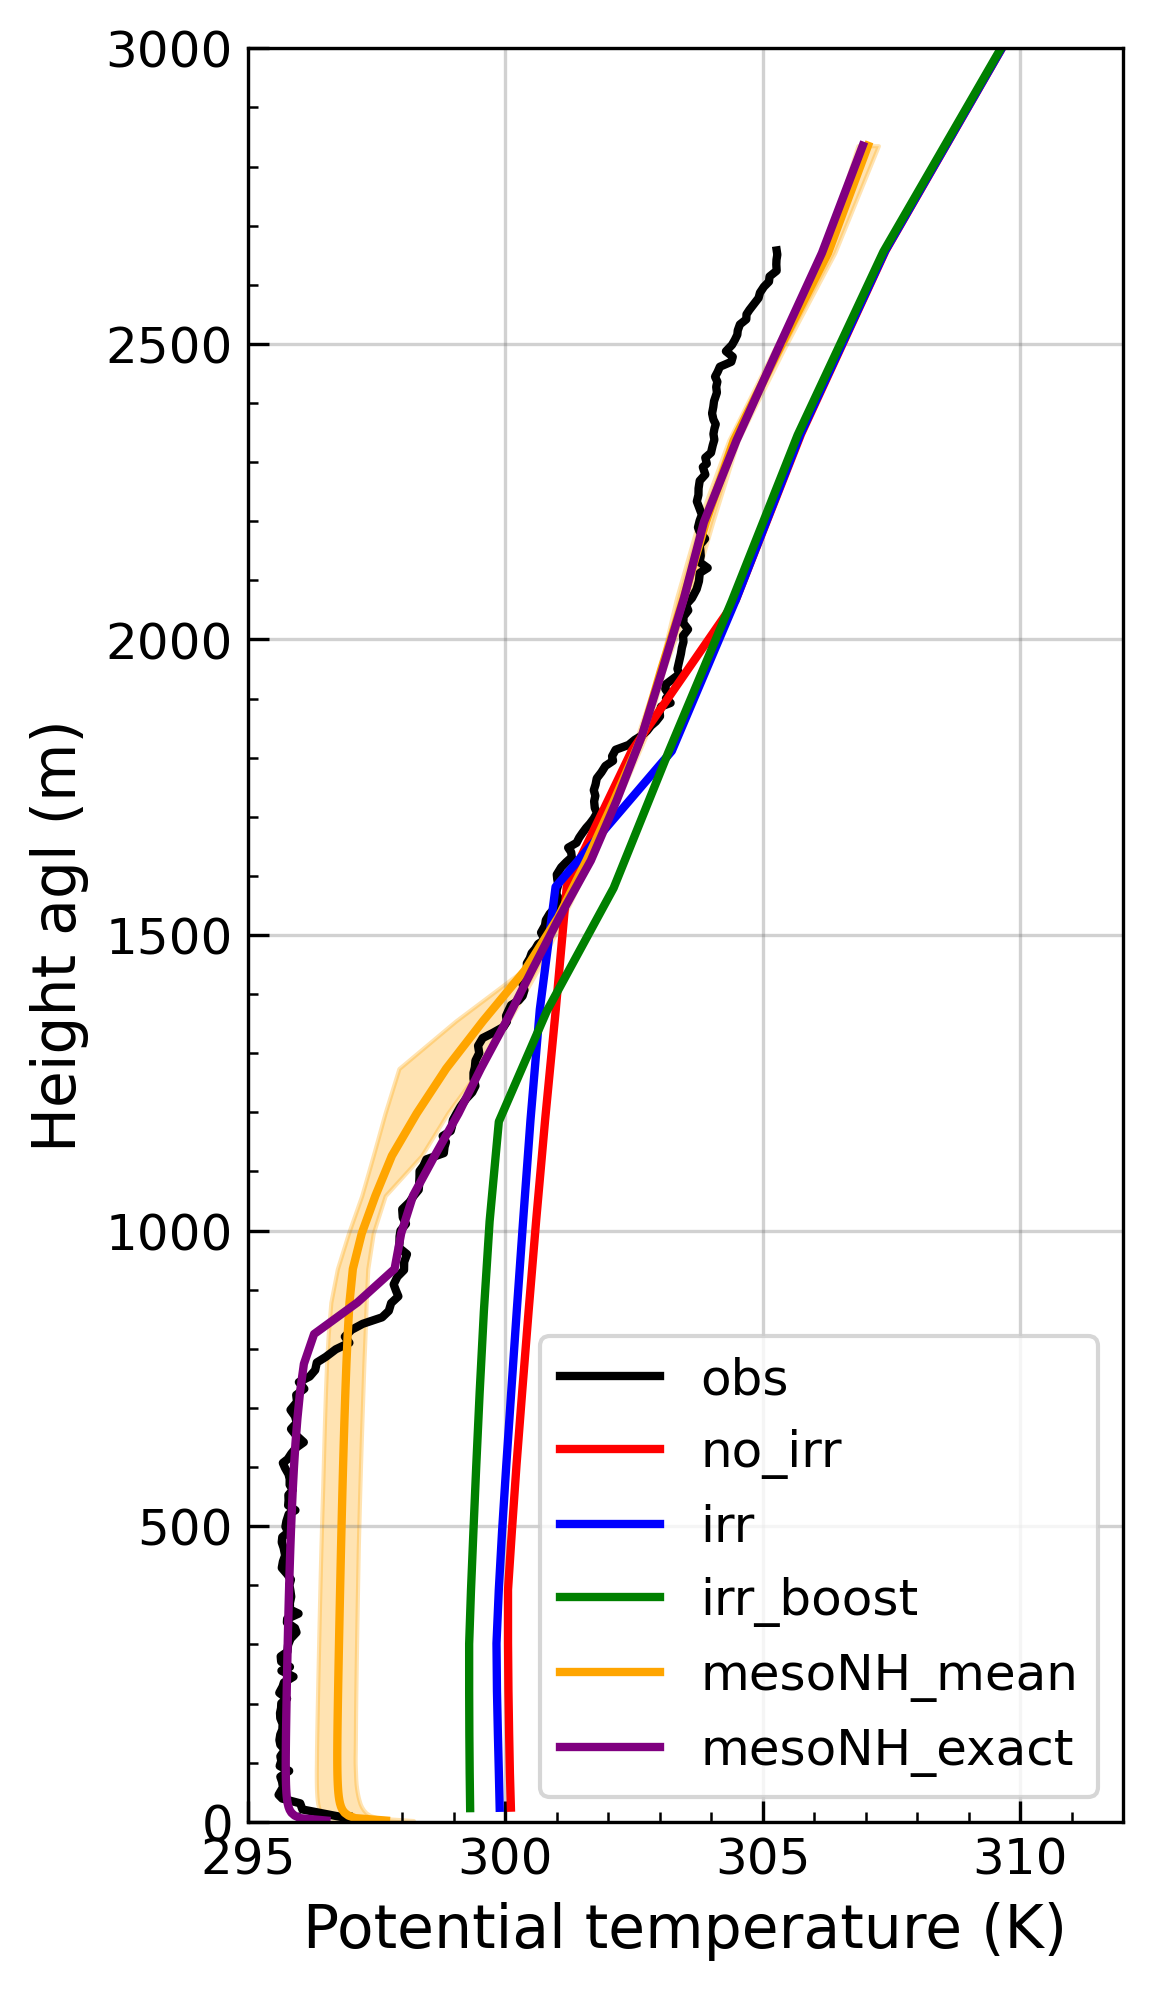
\includegraphics[width=\textwidth]{images/chap5/profiles/profile_cendrosa_theta_1507_.png}
        \end{subfigure} &
        \begin{subfigure}[t]{0.289\textwidth}
            \caption{}
            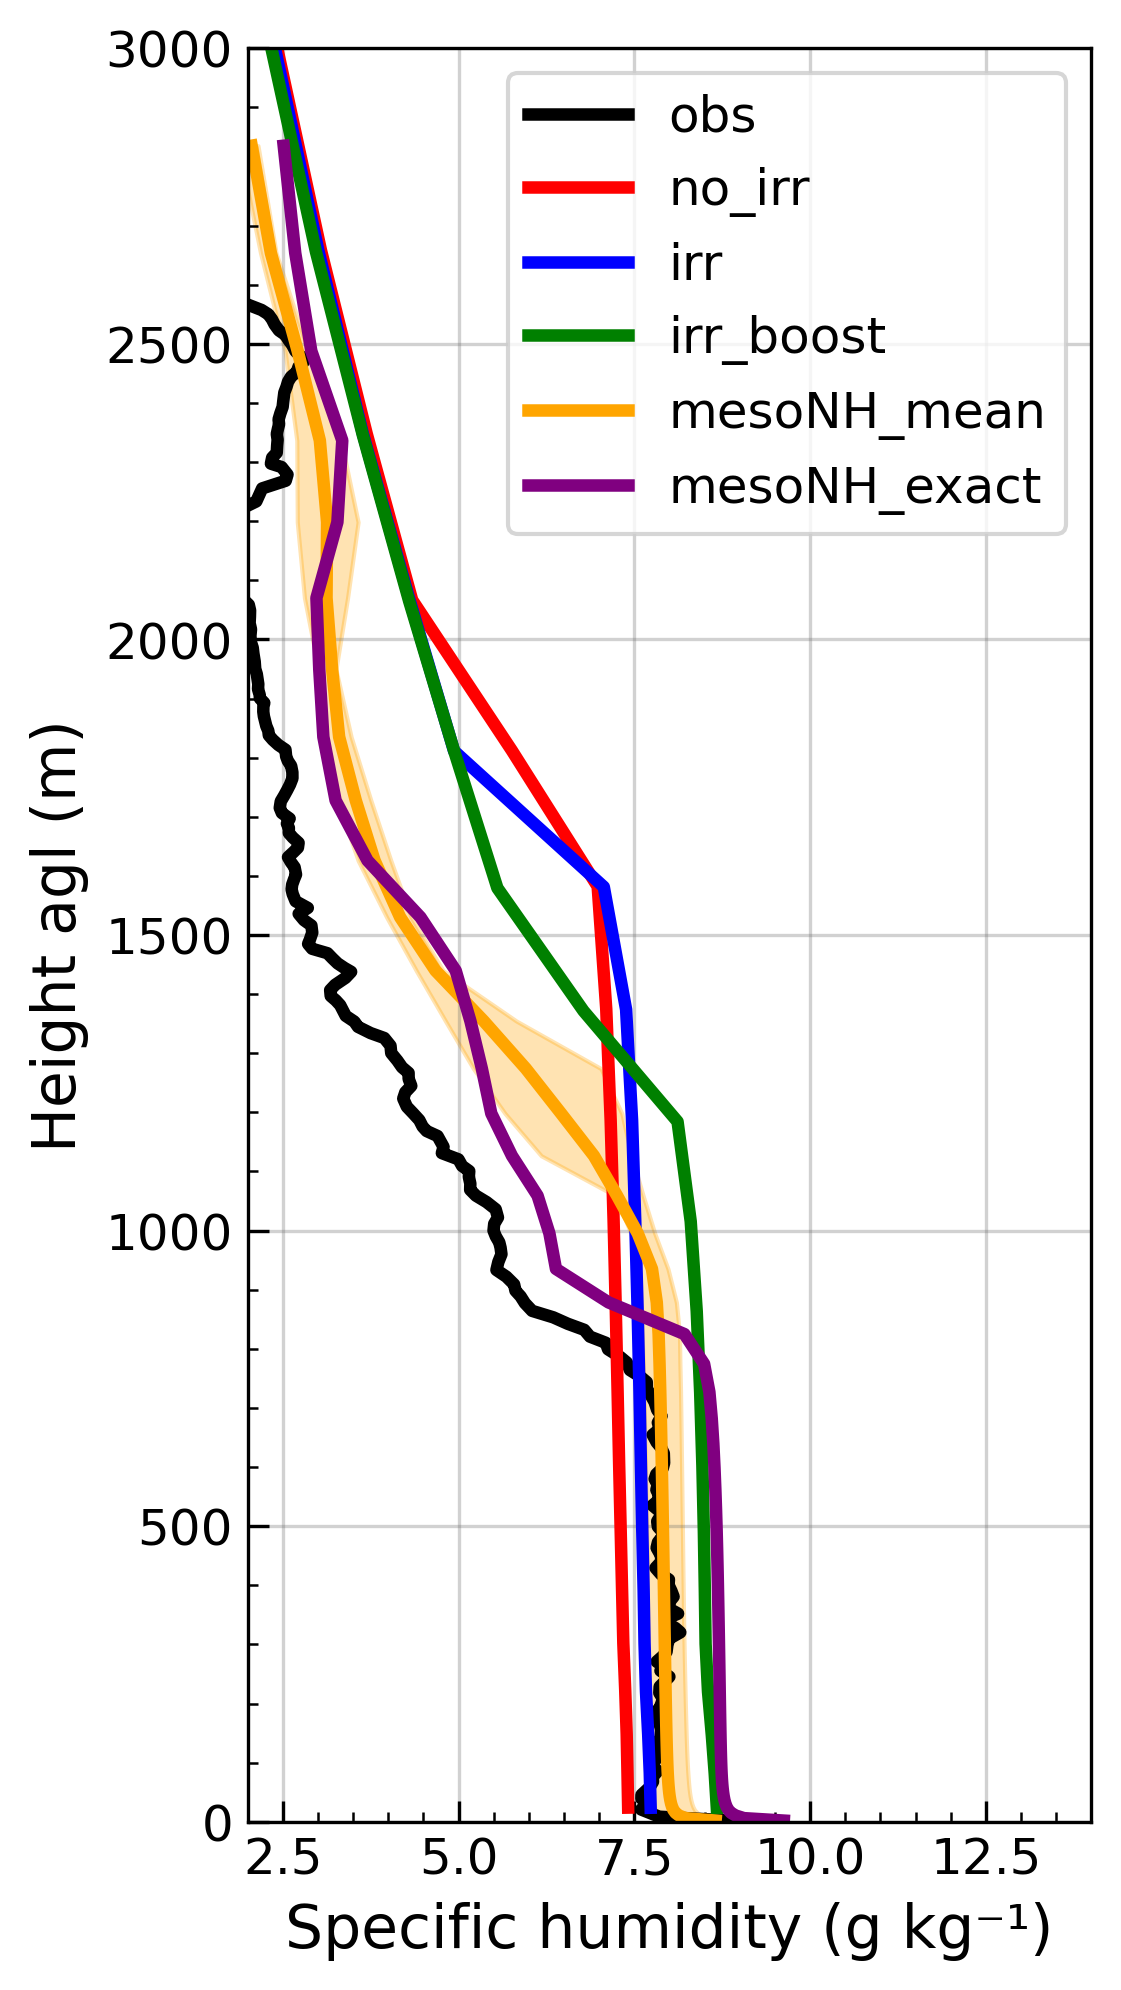
\includegraphics[width=\textwidth]{images/chap5/profiles/profile_cendrosa_ovap_1507_.png}
        \end{subfigure} &
        \begin{subfigure}[t]{0.283\textwidth}
            \caption{}
            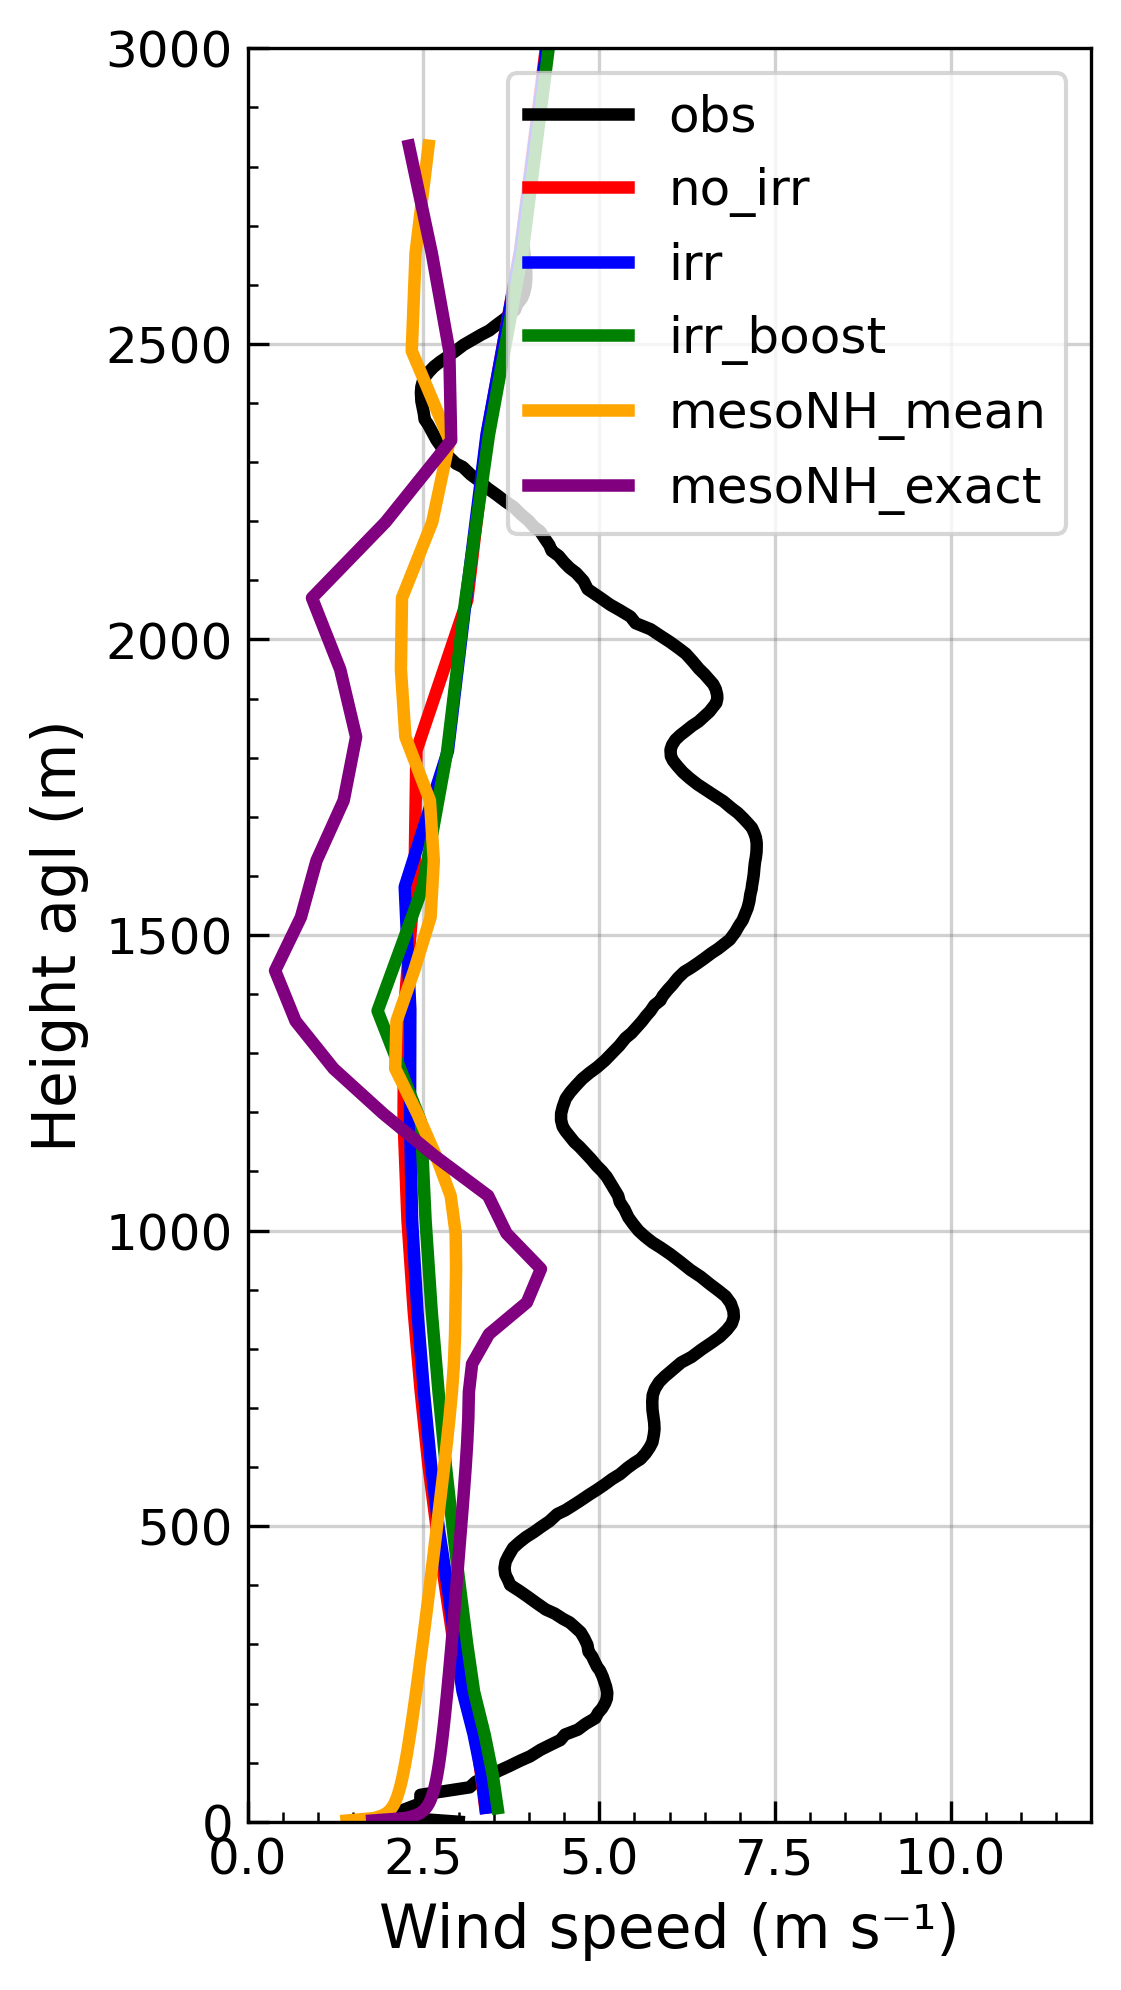
\includegraphics[width=\textwidth]{images/chap5/profiles/profile_cendrosa_wind_speed_1507_.png}
        \end{subfigure} &
        \begin{subfigure}[t]{0.283\textwidth}
            \caption{}
            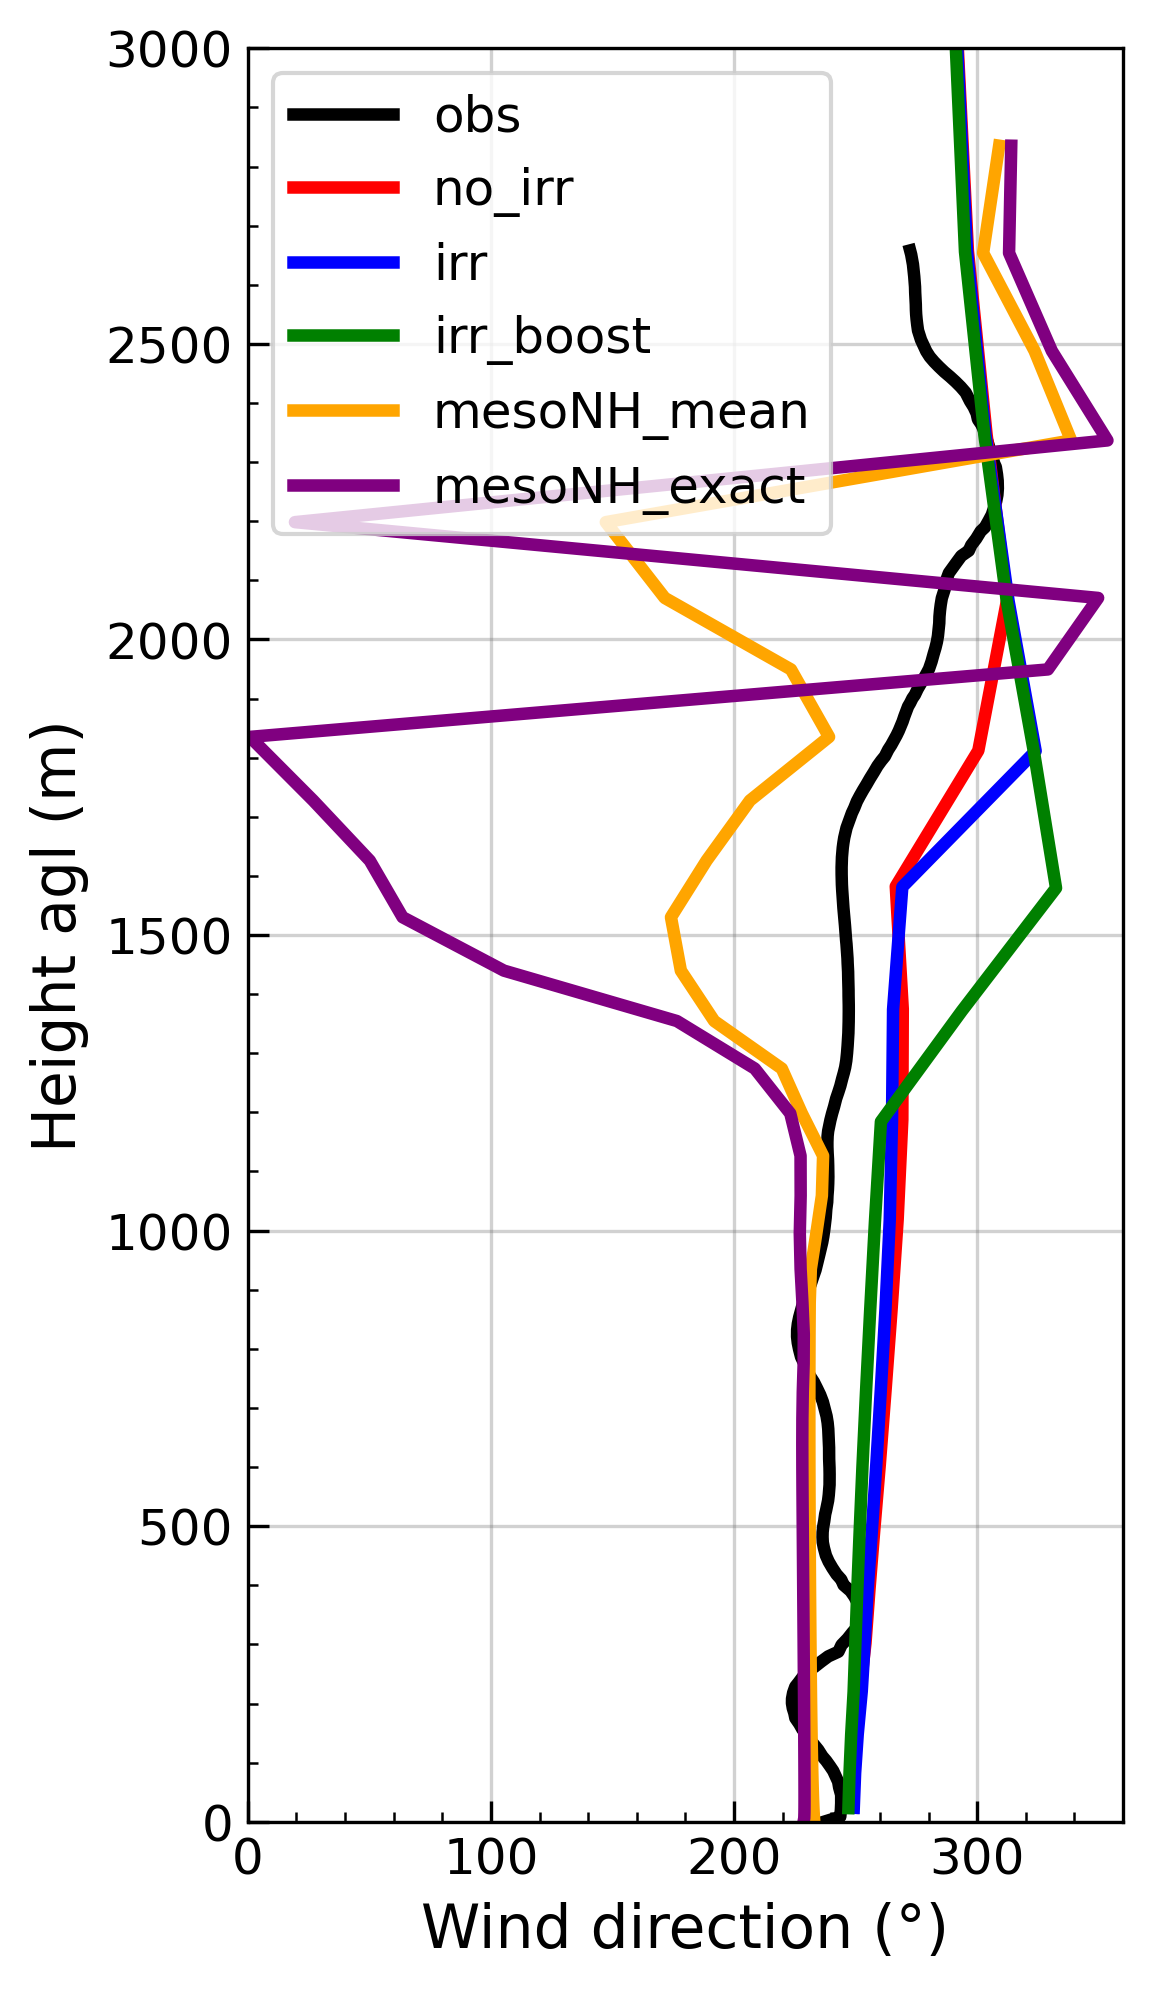
\includegraphics[width=\textwidth]{images/chap5/profiles/profile_cendrosa_wind_direction_1507_.png}
        \end{subfigure} \\
        %elsplans
        \begin{subfigure}[t]{0.382\textwidth}
            \caption{}
            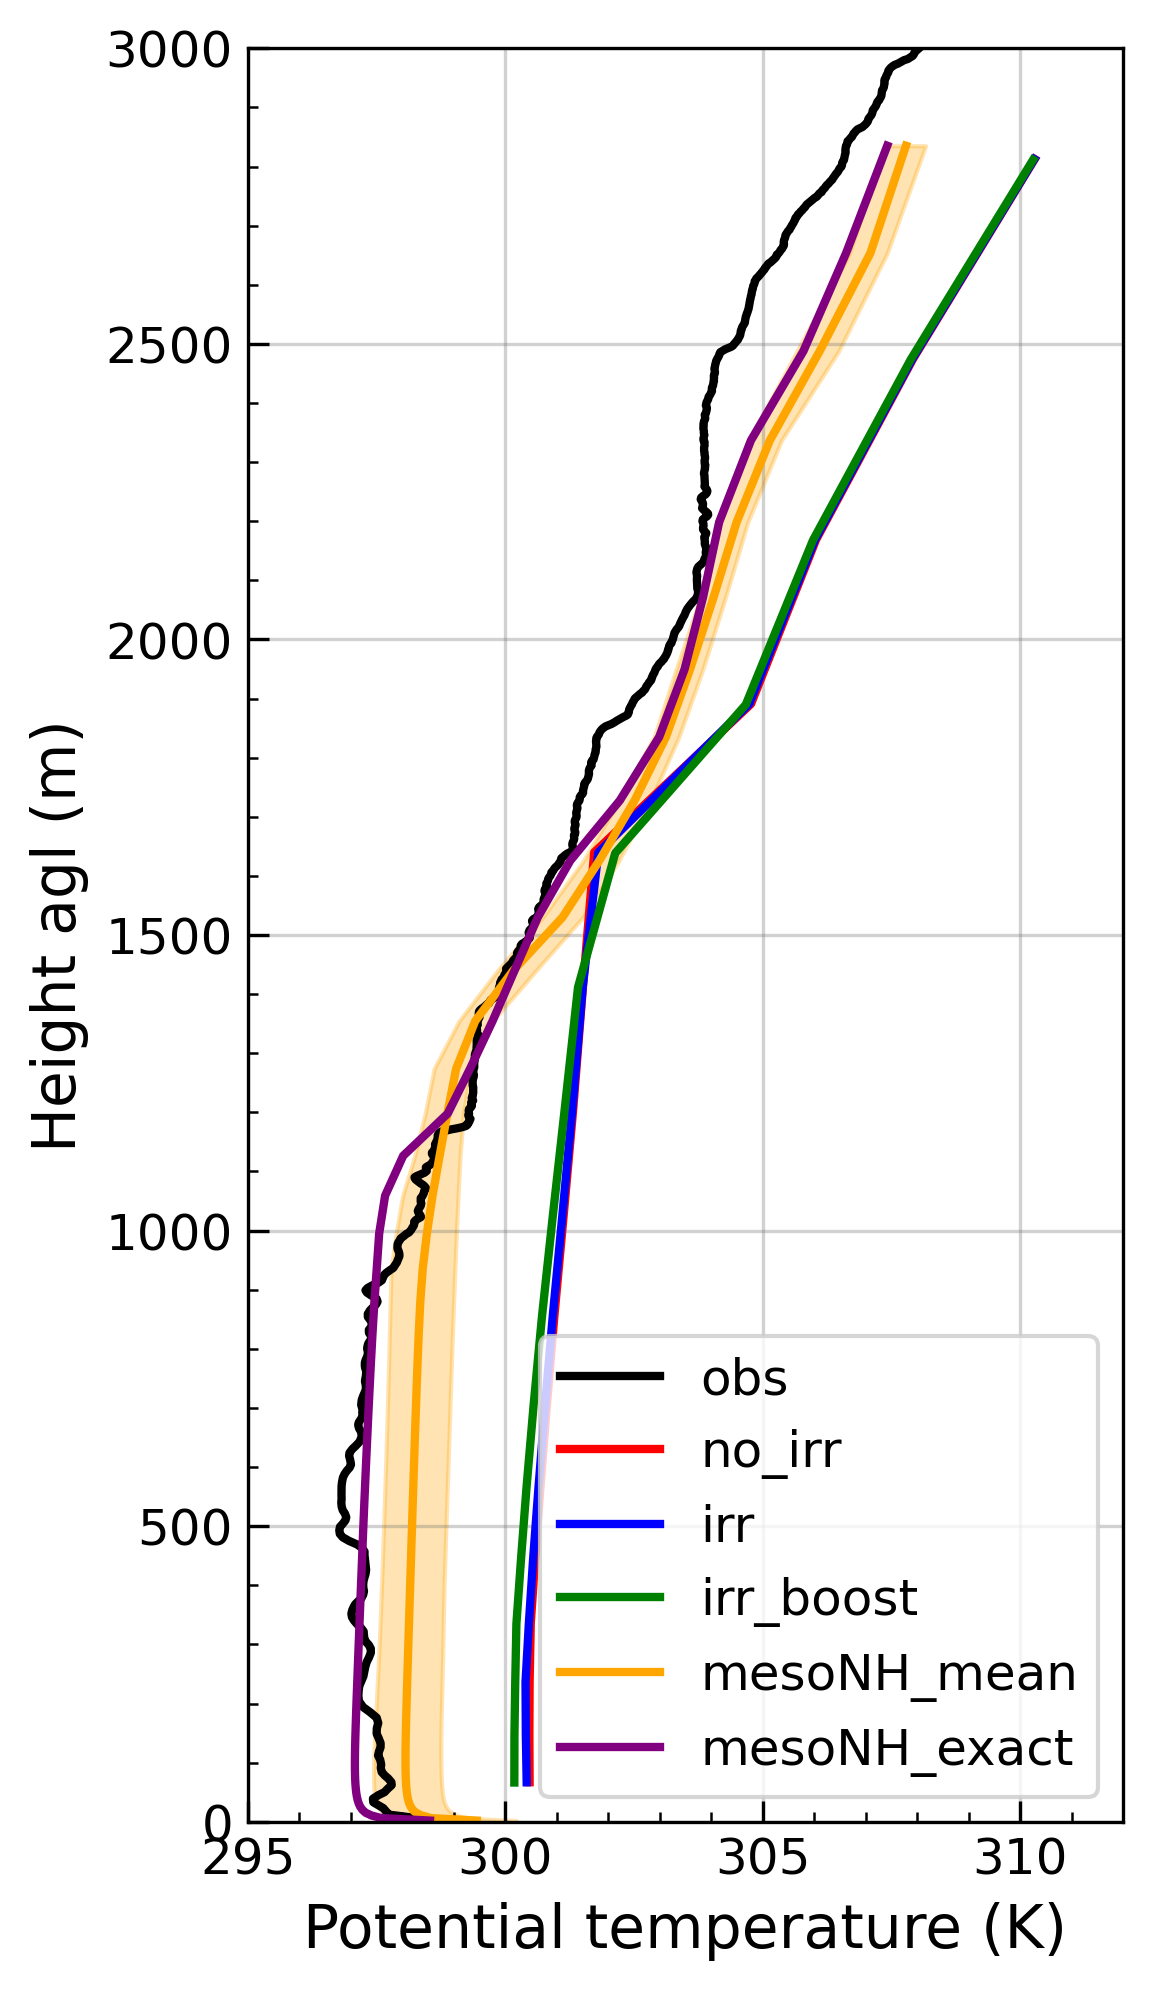
\includegraphics[width=\textwidth]{images/chap5/profiles/profile_elsplans_theta_1507_.png}
        \end{subfigure} &
        \begin{subfigure}[t]{0.289\textwidth}
            \caption{}
            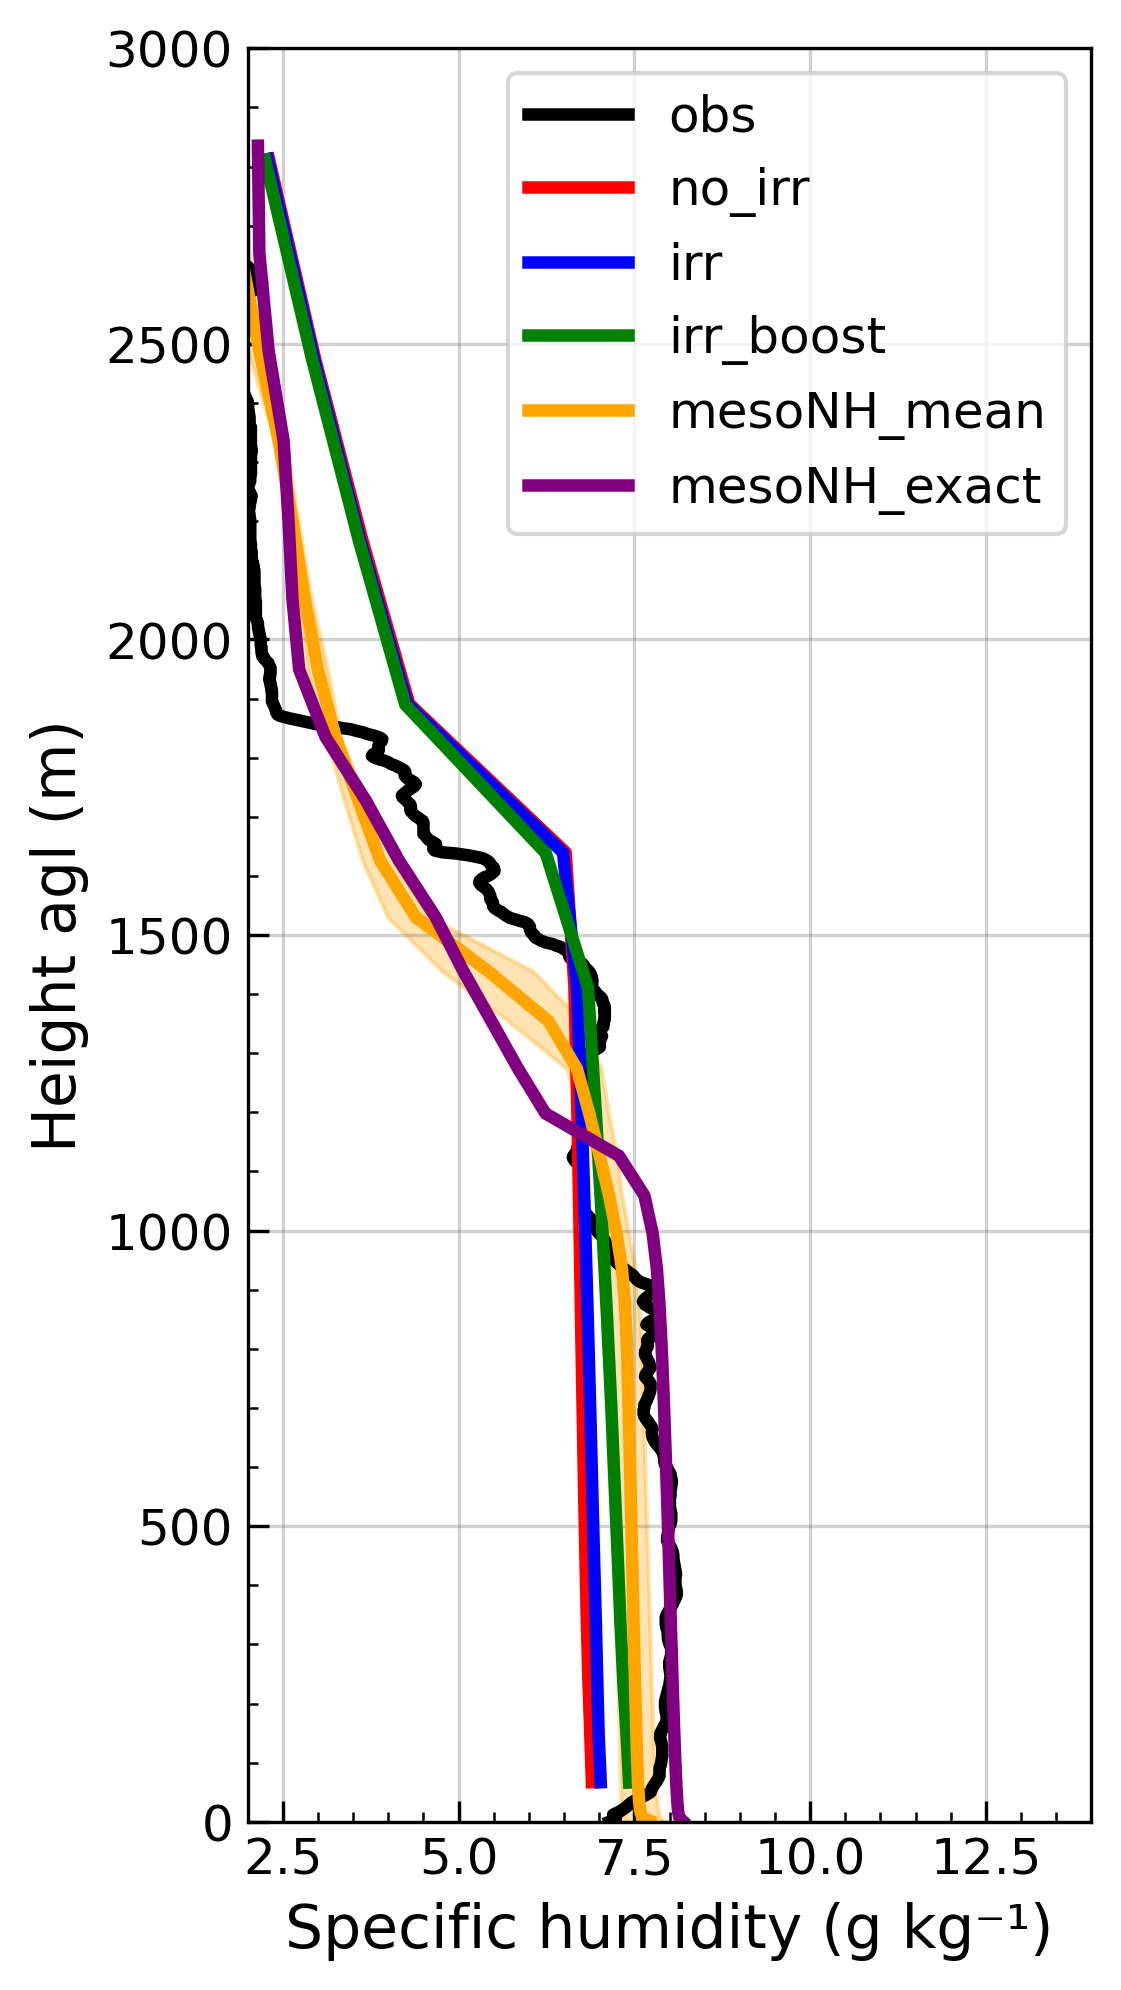
\includegraphics[width=\textwidth]{images/chap5/profiles/profile_elsplans_ovap_1507_.png}
        \end{subfigure} &
        \begin{subfigure}[t]{0.283\textwidth}
            \caption{}
            \includegraphics[width=\textwidth]{images/chap5/profiles/profile_elsplans_wind_speed_1507_.png}
        \end{subfigure} &
        \begin{subfigure}[t]{0.283\textwidth}
            \caption{}
            \includegraphics[width=\textwidth]{images/chap5/profiles/profile_elsplans_wind_direction_1507_.png}
        \end{subfigure} \\
    \end{tabular}
    }
    \caption{Vertical profiles at 12UTC on July 15th, at La Cendrosa (a-d) and Els Plans (e-h).}
    \label{fig:profiles_cendrosa_1507}
\end{figure}


%July 20th
%noirr : ABL too low (even more striking at els plans), although fsens strongly overestimated, consequence of dryness ?
%irrboost : reduces warm bias (half) and dry bias (matches obs but mesoMean even moister
%irrboost : lower ABL, making it worse...
%winds: link with ABL structure, missing lower jet at Els Plans

%Fig : profiles 2007 12UTC
\begin{figure}[hbtp]
    \centering
    \makebox[\textwidth][c]{%
    \begin{tabular}{@{}cccc@{}}
        %cendrosa
        \begin{subfigure}[t]{0.382\textwidth}
            \caption{}
            \includegraphics[width=\textwidth]{images/chap5/profiles/profile_cendrosa_theta_2007_.png}
        \end{subfigure} &
        \begin{subfigure}[t]{0.289\textwidth}
            \caption{}
            \includegraphics[width=\textwidth]{images/chap5/profiles/profile_cendrosa_ovap_2007_.png}
        \end{subfigure} &
        \begin{subfigure}[t]{0.283\textwidth}
            \caption{}
            \includegraphics[width=\textwidth]{images/chap5/profiles/profile_cendrosa_wind_speed_2007_.png}
        \end{subfigure} &
        \begin{subfigure}[t]{0.283\textwidth}
            \caption{}
            \includegraphics[width=\textwidth]{images/chap5/profiles/profile_cendrosa_wind_direction_2007_.png}
        \end{subfigure} \\
        %elsplans
        \begin{subfigure}[t]{0.382\textwidth}
            \caption{}
            \includegraphics[width=\textwidth]{images/chap5/profiles/profile_elsplans_theta_2007_.png}
        \end{subfigure} &
        \begin{subfigure}[t]{0.289\textwidth}
            \caption{}
            \includegraphics[width=\textwidth]{images/chap5/profiles/profile_elsplans_ovap_2007_.png}
        \end{subfigure} &
        %winds
        \begin{subfigure}[t]{0.283\textwidth}
            \caption{}
            \includegraphics[width=\textwidth]{images/chap5/profiles/profile_elsplans_wind_speed_2007_.png}
        \end{subfigure} &
        \begin{subfigure}[t]{0.283\textwidth}
            \caption{}
            \includegraphics[width=\textwidth]{images/chap5/profiles/profile_elsplans_wind_direction_2007_.png}
        \end{subfigure} \\
    \end{tabular}
    }
    \caption{Vertical profiles at 12UTC on July 20th, at La Cendrosa (a-d) and Els Plans (e-h).}
    \label{fig:profiles_cendrosa_2007}
\end{figure}

\clearpage

\section{Importance of surface fluxes heterogeneities}

\clearpage
\section{Chapter conclusions}
%irrigation without boost does not have very significant impact
%with boostirr, manage to get much closer to observations 

%no impact on Els Plans site, not a surprise
\clearpage
\section{Chapter appendix}

\begin{figure}[hbtp]
    \centering
    \begin{tabular}{cc}
        \begin{subfigure}[t]{0.5\textwidth}
            \caption{}
            \includegraphics[width=\textwidth]{images/chap5/SOP_TS_DC/time_series_cendrosa_SWdnSFC.png}
        \end{subfigure} &
        \begin{subfigure}[t]{0.5\textwidth}
            \caption{}
            \includegraphics[width=\textwidth]{images/chap5/SOP_TS_DC/diurnal_cycle_cendrosa_SWdnSFC.png}
        \end{subfigure} \\
        
        \begin{subfigure}[t]{0.5\textwidth}
            \caption{}
            \includegraphics[width=\textwidth]{images/chap5/SOP_TS_DC/time_series_cendrosa_LWdnSFC.png}
        \end{subfigure} &
        \begin{subfigure}[t]{0.5\textwidth}
            \caption{}
            \includegraphics[width=\textwidth]{images/chap5/SOP_TS_DC/diurnal_cycle_cendrosa_LWdnSFC.png}
        \end{subfigure} \\

        \begin{subfigure}[t]{0.5\textwidth}
            \caption{}
            \includegraphics[width=\textwidth]{images/chap5/SOP_TS_DC/time_series_elsplans_SWdnSFC.png}
        \end{subfigure} &
        \begin{subfigure}[t]{0.5\textwidth}
            \caption{}
            \includegraphics[width=\textwidth]{images/chap5/SOP_TS_DC/diurnal_cycle_elsplans_SWdnSFC.png}
        \end{subfigure} \\
        
        \begin{subfigure}[t]{0.5\textwidth}
            \caption{}
            \includegraphics[width=\textwidth]{images/chap5/SOP_TS_DC/time_series_elsplans_LWdnSFC.png}
        \end{subfigure} &
        \begin{subfigure}[t]{0.5\textwidth}
            \caption{}
            \includegraphics[width=\textwidth]{images/chap5/SOP_TS_DC/diurnal_cycle_elsplans_LWdnSFC.png}
        \end{subfigure} \\
    \end{tabular}
    \caption{Time series and mean diurnal cycle of radiative fluxes on both sites, July 14-30 2021.}
    \label{fig:bothsites_rad}
\end{figure}


%Fig : energy fluxes ElsPlans
\begin{figure}[hbtp]
    \centering
    \begin{tabular}{cc}
        %rad fluxes
        \begin{subfigure}[t]{0.5\textwidth}
            \caption{}
            \includegraphics[width=\textwidth]{images/chap5/IOP_TS/TS_2021-07-15_elsplans_SWdnSFC.png}
        \end{subfigure} &
        \begin{subfigure}[t]{0.5\textwidth}
            \caption{}
            \includegraphics[width=\textwidth]{images/chap5/IOP_TS/TS_2021-07-20_elsplans_SWdnSFC.png}
        \end{subfigure} \\
        \begin{subfigure}[t]{0.5\textwidth}
            \caption{}
            \includegraphics[width=\textwidth]{images/chap5/IOP_TS/TS_2021-07-15_elsplans_LWdnSFC.png}
        \end{subfigure} &
        \begin{subfigure}[t]{0.5\textwidth}
            \caption{}
            \includegraphics[width=\textwidth]{images/chap5/IOP_TS/TS_2021-07-20_elsplans_LWdnSFC.png}
        \end{subfigure} \\

        %turb fluxes
        \begin{subfigure}[t]{0.5\textwidth}
            \caption{}
            \includegraphics[width=\textwidth]{images/chap5/IOP_TS/TS_2021-07-15_elsplans_flat.png}
        \end{subfigure} &
        \begin{subfigure}[t]{0.5\textwidth}
            \caption{}
            \includegraphics[width=\textwidth]{images/chap5/IOP_TS/TS_2021-07-20_elsplans_flat.png}
        \end{subfigure} \\
        \begin{subfigure}[t]{0.5\textwidth}
            \caption{}
            \includegraphics[width=\textwidth]{images/chap5/IOP_TS/TS_2021-07-15_elsplans_sens.png}
        \end{subfigure} &
        \begin{subfigure}[t]{0.5\textwidth}
            \caption{}
            \includegraphics[width=\textwidth]{images/chap5/IOP_TS/TS_2021-07-20_elsplans_sens.png}
        \end{subfigure} \\
    \end{tabular}
    \caption{}
    \label{fig:iop_days_TS_energy_elsplans}
\end{figure}

%Fig : surface variables ElsPlans
\begin{figure}[hbtp]
    \centering
    \begin{tabular}{cc}
        %t2m, q2m
        \begin{subfigure}[t]{0.5\textwidth}
            \caption{}
            \includegraphics[width=\textwidth]{images/chap5/IOP_TS/TS_2021-07-15_elsplans_t2m.png}
        \end{subfigure} &
        \begin{subfigure}[t]{0.5\textwidth}
            \caption{}
            \includegraphics[width=\textwidth]{images/chap5/IOP_TS/TS_2021-07-20_elsplans_t2m.png}
        \end{subfigure} \\
        \begin{subfigure}[t]{0.5\textwidth}
            \caption{}
            \includegraphics[width=\textwidth]{images/chap5/IOP_TS/TS_2021-07-15_elsplans_q2m.png}
        \end{subfigure} &
        \begin{subfigure}[t]{0.5\textwidth}
            \caption{}
            \includegraphics[width=\textwidth]{images/chap5/IOP_TS/TS_2021-07-20_elsplans_q2m.png}
        \end{subfigure} \\

        %turb fluxes
        \begin{subfigure}[t]{0.5\textwidth}
            \caption{}
            \includegraphics[width=\textwidth]{images/chap5/IOP_TS/TS_2021-07-15_elsplans_wind_speed_10m.png}
        \end{subfigure} &
        \begin{subfigure}[t]{0.5\textwidth}
            \caption{}
            \includegraphics[width=\textwidth]{images/chap5/IOP_TS/TS_2021-07-20_elsplans_wind_speed_10m.png}
        \end{subfigure} \\
        \begin{subfigure}[t]{0.5\textwidth}
            \caption{}
            \includegraphics[width=\textwidth]{images/chap5/IOP_TS/TS_2021-07-15_elsplans_wind_direction_10m.png}
        \end{subfigure} &
        \begin{subfigure}[t]{0.5\textwidth}
            \caption{}
            \includegraphics[width=\textwidth]{images/chap5/IOP_TS/TS_2021-07-20_elsplans_wind_direction_10m.png}
        \end{subfigure} \\
    \end{tabular}
    \caption{}
    \label{fig:iop_days_TS_surfvars_elsplans}
\end{figure}



%todo:relocate appendix